Figure \ref{fig:img3} shows the original image with some kind of white noise in it, and by analysing the image histogram (image \ref{fig:img3_hist}) can two kind of noise fit this: Gaussian noise (figure \ref{fig:noise_gaussian}) and uniform noise (figure \ref{fig:noise_uniform}).

\begin{figure}[H]
    \centering
    \begin{subfigure}[b]{0.25\textwidth}
        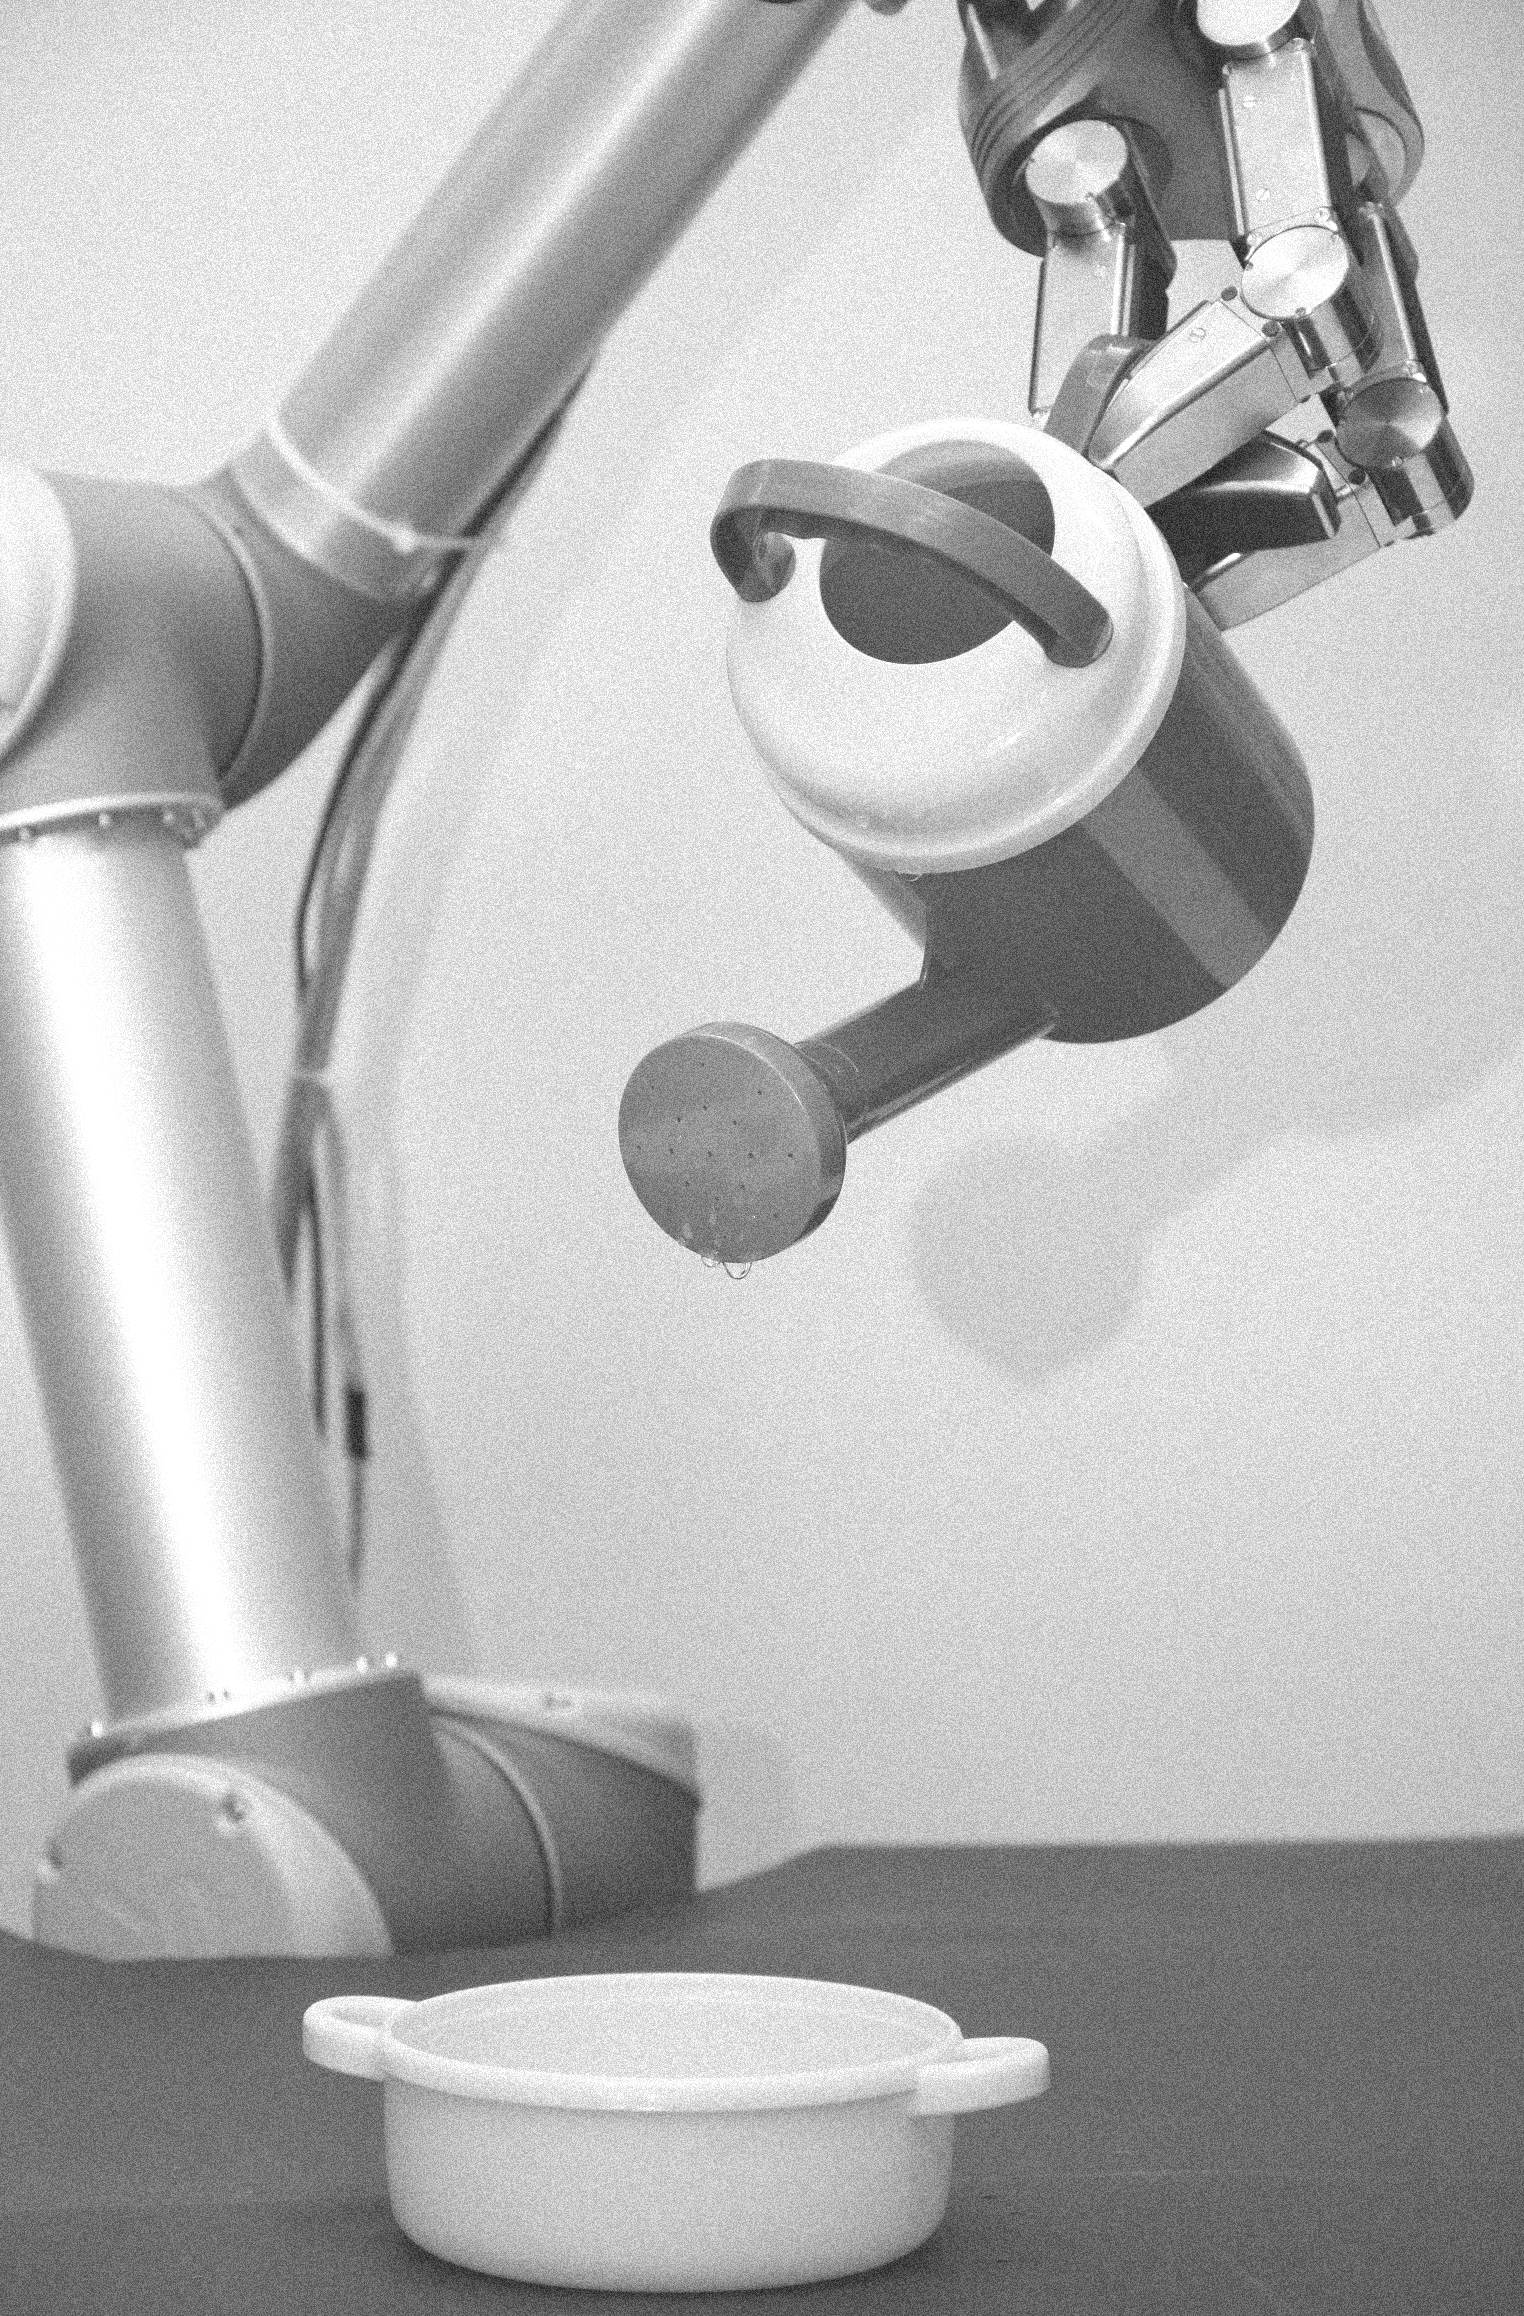
\includegraphics[width=\textwidth]{img3/src.png}
        \caption{The original image}
        \label{fig:img3_src}
    \end{subfigure}
    \begin{subfigure}[b]{0.485\textwidth}
        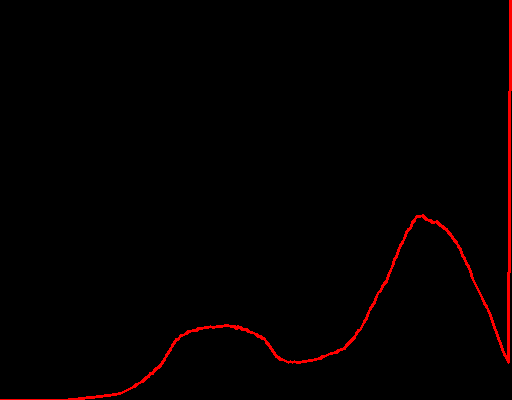
\includegraphics[width=\textwidth]{img3/hist_org_img3.png}
        \caption{Histogram of the original image}
        \label{fig:img3_hist}
    \end{subfigure}
    \caption{Analysis of image 3}
    \label{fig:img3}
\end{figure}
In order to determine which kind of noise it is, an uniform surface of the image is analysed, as shown on figure \todo{Vi har vel tjekket alle  histogram for alle i uniforme overflader.. Det vel en selvfølge, så vi burde nok skrive det et sted..} \ref{fig:rect_org_img3}. By comparing the histogram of the uniform surface in figure \ref{fig:rect_org_img3} with the two noise examples histograms in figure \ref{fig:noise_examples_img3}, it can be determined that as the noise in image \ref{fig:img3_src} mostly resembles uniform noise,   it is also present in the image . 

\begin{figure}[H]
    \centering
    \begin{subfigure}[b]{0.22\textwidth}
        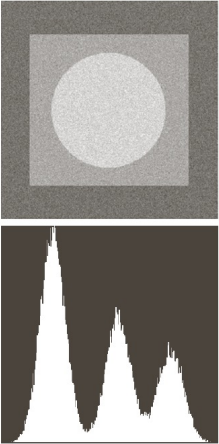
\includegraphics[width=\textwidth]{img3/noise_g.png}
        \caption{Gaussian noise}
        \label{fig:noise_gaussian}
    \end{subfigure}
    \begin{subfigure}[b]{0.2175\textwidth}
        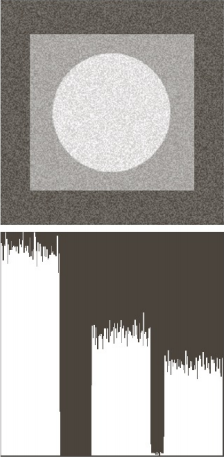
\includegraphics[width=\textwidth]{img3/noise_u.png}
        \caption{Uniform noise}
        \label{fig:noise_uniform}
    \end{subfigure}
    \caption{Examples of different noise models}
    \label{fig:noise_examples_img3}
\end{figure}

\begin{figure}[H]
    \centering
    \begin{subfigure}[b]{0.24\textwidth}
        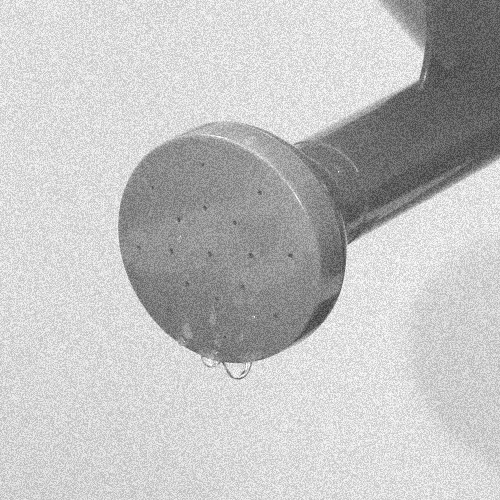
\includegraphics[width=\textwidth]{img3/rect_org_img3.png}
        \begin{center}
        	\textbf{Uniform surfaces}
        \end{center}
        
\includegraphics[width=\textwidth]{img3/rect_src_img3.png}\\[0.1cm]
        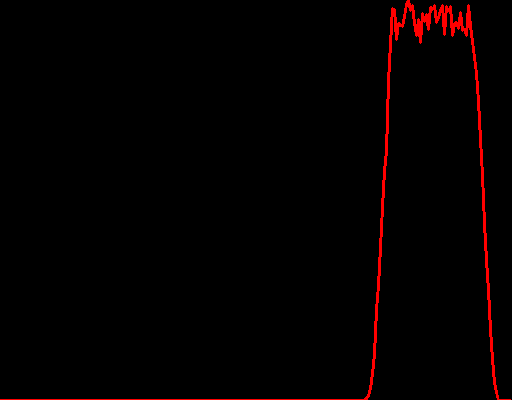
\includegraphics[width=\textwidth]{img3/hist_rect_src_img3.png}
        \caption{The original image}
        \label{fig:rect_org_img3}
    \end{subfigure}
    \begin{subfigure}[b]{0.24\textwidth}
        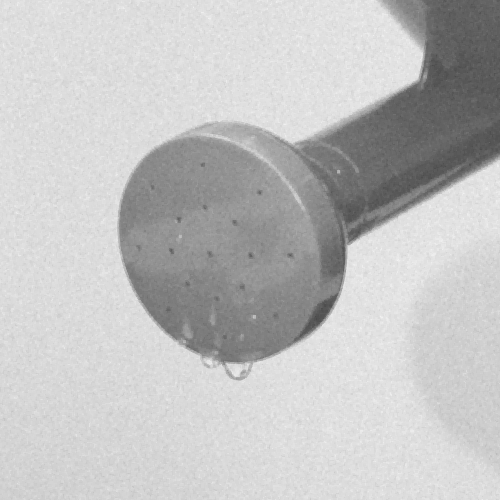
\includegraphics[width=\textwidth]{img3/rect_3_midpoint_3_final_img3_add.png}
        \begin{center}
        	\text{ }
        \end{center}
        
\includegraphics[width=\textwidth]{img3/rect_3_midpoint_3_final_img3.png}\\[0.1cm]
        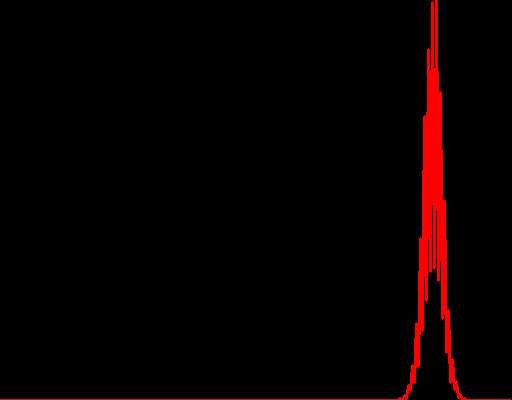
\includegraphics[width=\textwidth]{img3/hist_rect_3_midpoint_3_final_img3.png}
        \caption{Kernel 3}
        \label{fig:img3_kernel_3}
    \end{subfigure}
    \begin{subfigure}[b]{0.24\textwidth}
        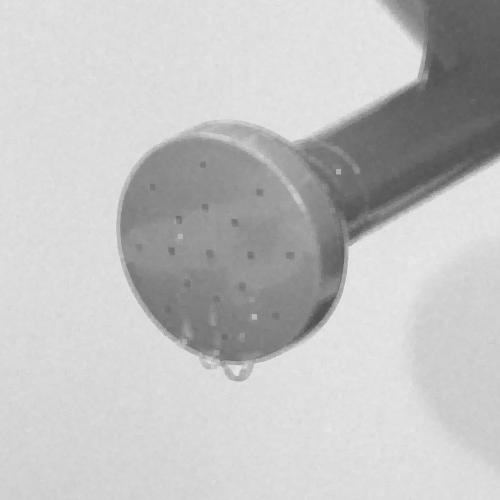
\includegraphics[width=\textwidth]{img3/rect_5_midpoint_5_final_img3_add.png}
        \begin{center}
        	\text{ }
        \end{center}
        
\includegraphics[width=\textwidth]{img3/rect_5_midpoint_5_final_img3.png}\\[0.1cm]
        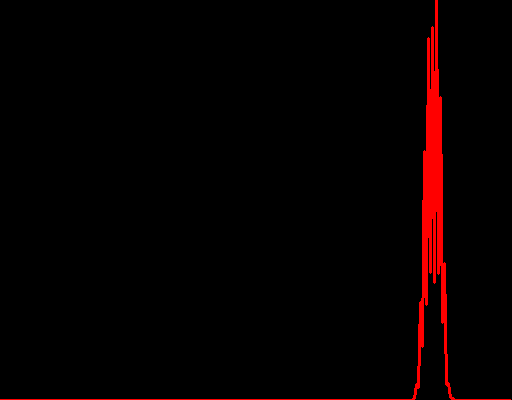
\includegraphics[width=\textwidth]{img3/hist_rect_5_midpoint_5_final_img3.png}
        \caption{Kernel 5}
        \label{fig:img3_kernel_5}
    \end{subfigure}
    \begin{subfigure}[b]{0.24\textwidth}
        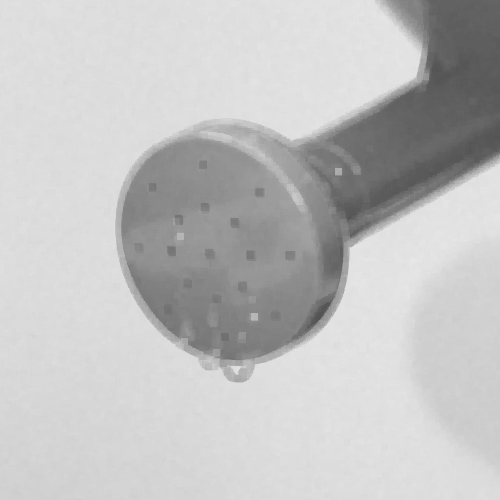
\includegraphics[width=\textwidth]{img3/rect_7_midpoint_7_final_img3_add.png}
        \begin{center}
        	\text{ }
        \end{center}
        
\includegraphics[width=\textwidth]{img3/rect_7_midpoint_7_final_img3.png}\\[0.1cm]
        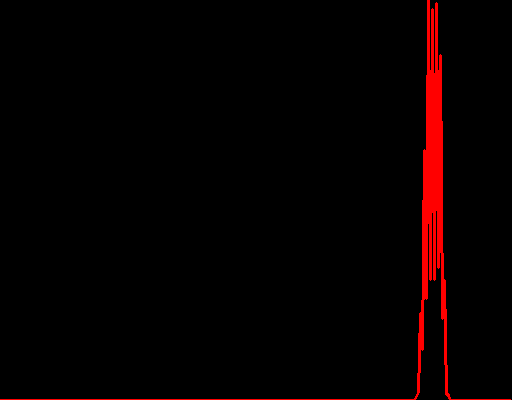
\includegraphics[width=\textwidth]{img3/hist_rect_7_midpoint_7_final_img3.png}
        \caption{Kernel 7}
        \label{fig:img3_kernel_7}
    \end{subfigure}
    \caption{Analysis of image 3}
    \label{fig:img3_kernel}
\end{figure}

In order to reduce the uniform noise in the image, a midpoint filter is applied to the image, as it is effective against Gaussian noise and uniform noise \todo{ref}. The method works be replacing the pixel with the average value (i.e. the midpoint) of the minimum pixel and maximum pixel within an kernel.  The kernel size must be odd and greater than 1, and the greater the kernel size is, the greater are the effects , but the image becomes more pixelated especially at the edges.  \\[0.2cm]
Figure \ref{fig:img3_kernel_3}, \ref{fig:img3_kernel_5} and \ref{fig:img3_kernel_7} shows the result of three different kernel sizes; 3, 5 and 7. By comparing the same uniform surface of each of the images, can it be seen that a kernel 3 does not remove all the noise, but kernel 5 and 7 does. By comparing the sharpness of the edges with a kernel 5 and a kernel 7, the kernel 7's edges is too pixelated compared to the edges in kernel 5, and that is why in this project a midpoint filter with a kernel 5 is chosen to be applied in order to remove the uniform noise in image \ref{fig:img3_src}.\\[0.2cm]
Figure \ref{fig:img3_kernel_5_final} shows the full image after applying the midpoint filter with a kernel size of 5, and compared to the original image (figure \ref{fig:img3_org_final}) it can be seen that there is a difference in the brightness. Figure \ref{fig:img3_kernel_5_final} is brighter than the original image, and therefore is the OpenCV function used
\begin{center}
\lstinline|void Mat::convertTo(OutputArray m, int rtype, double alpha=1, double beta=0 )|\footnote{\url{http://docs.opencv.org/2.4/modules/core/doc/basic_structures.html\#mat-convertto}}
\end{center}
and by changing the \lstinline|alpha| is it possible equalizing the brightness between the source image and the original image as much as possible. An \lstinline|alpha| lower than 1 will darken the image, and an \lstinline|alpha| higher than 1 will brighten the image. Figure \ref{fig:img3_test_brightness} shows the result of some different values of \lstinline|aplha|, where the first row is an \lstinline|alpha| value below 1 and the second row is an \lstinline|alpha| above 1. Finding the right \lstinline|alpha| is done by testing with different values below 1, similar to the first row in figure \ref{fig:img3_test_brightness}, with an step of 0.05, and the best fit was found to be an \lstinline|alphe=0.85|, so 
\begin{center}
\lstinline|scr.convertTo(dst, -1, 0.85, 0)|
\end{center}
and the result of this is shown on figure \ref{fig:img3_contrast}. After this equalization  of the brightness can it also be seen that the full histogram of figure \ref{fig:img3_contrast} look a lot more similar to figure \ref{fig:img3_org_final}'s full histogram, compared to figure \ref{fig:img3_kernel_5_final}'s histogram.

\begin{figure}[H]
    \centering
    \begin{subfigure}[b]{0.1\textwidth}
        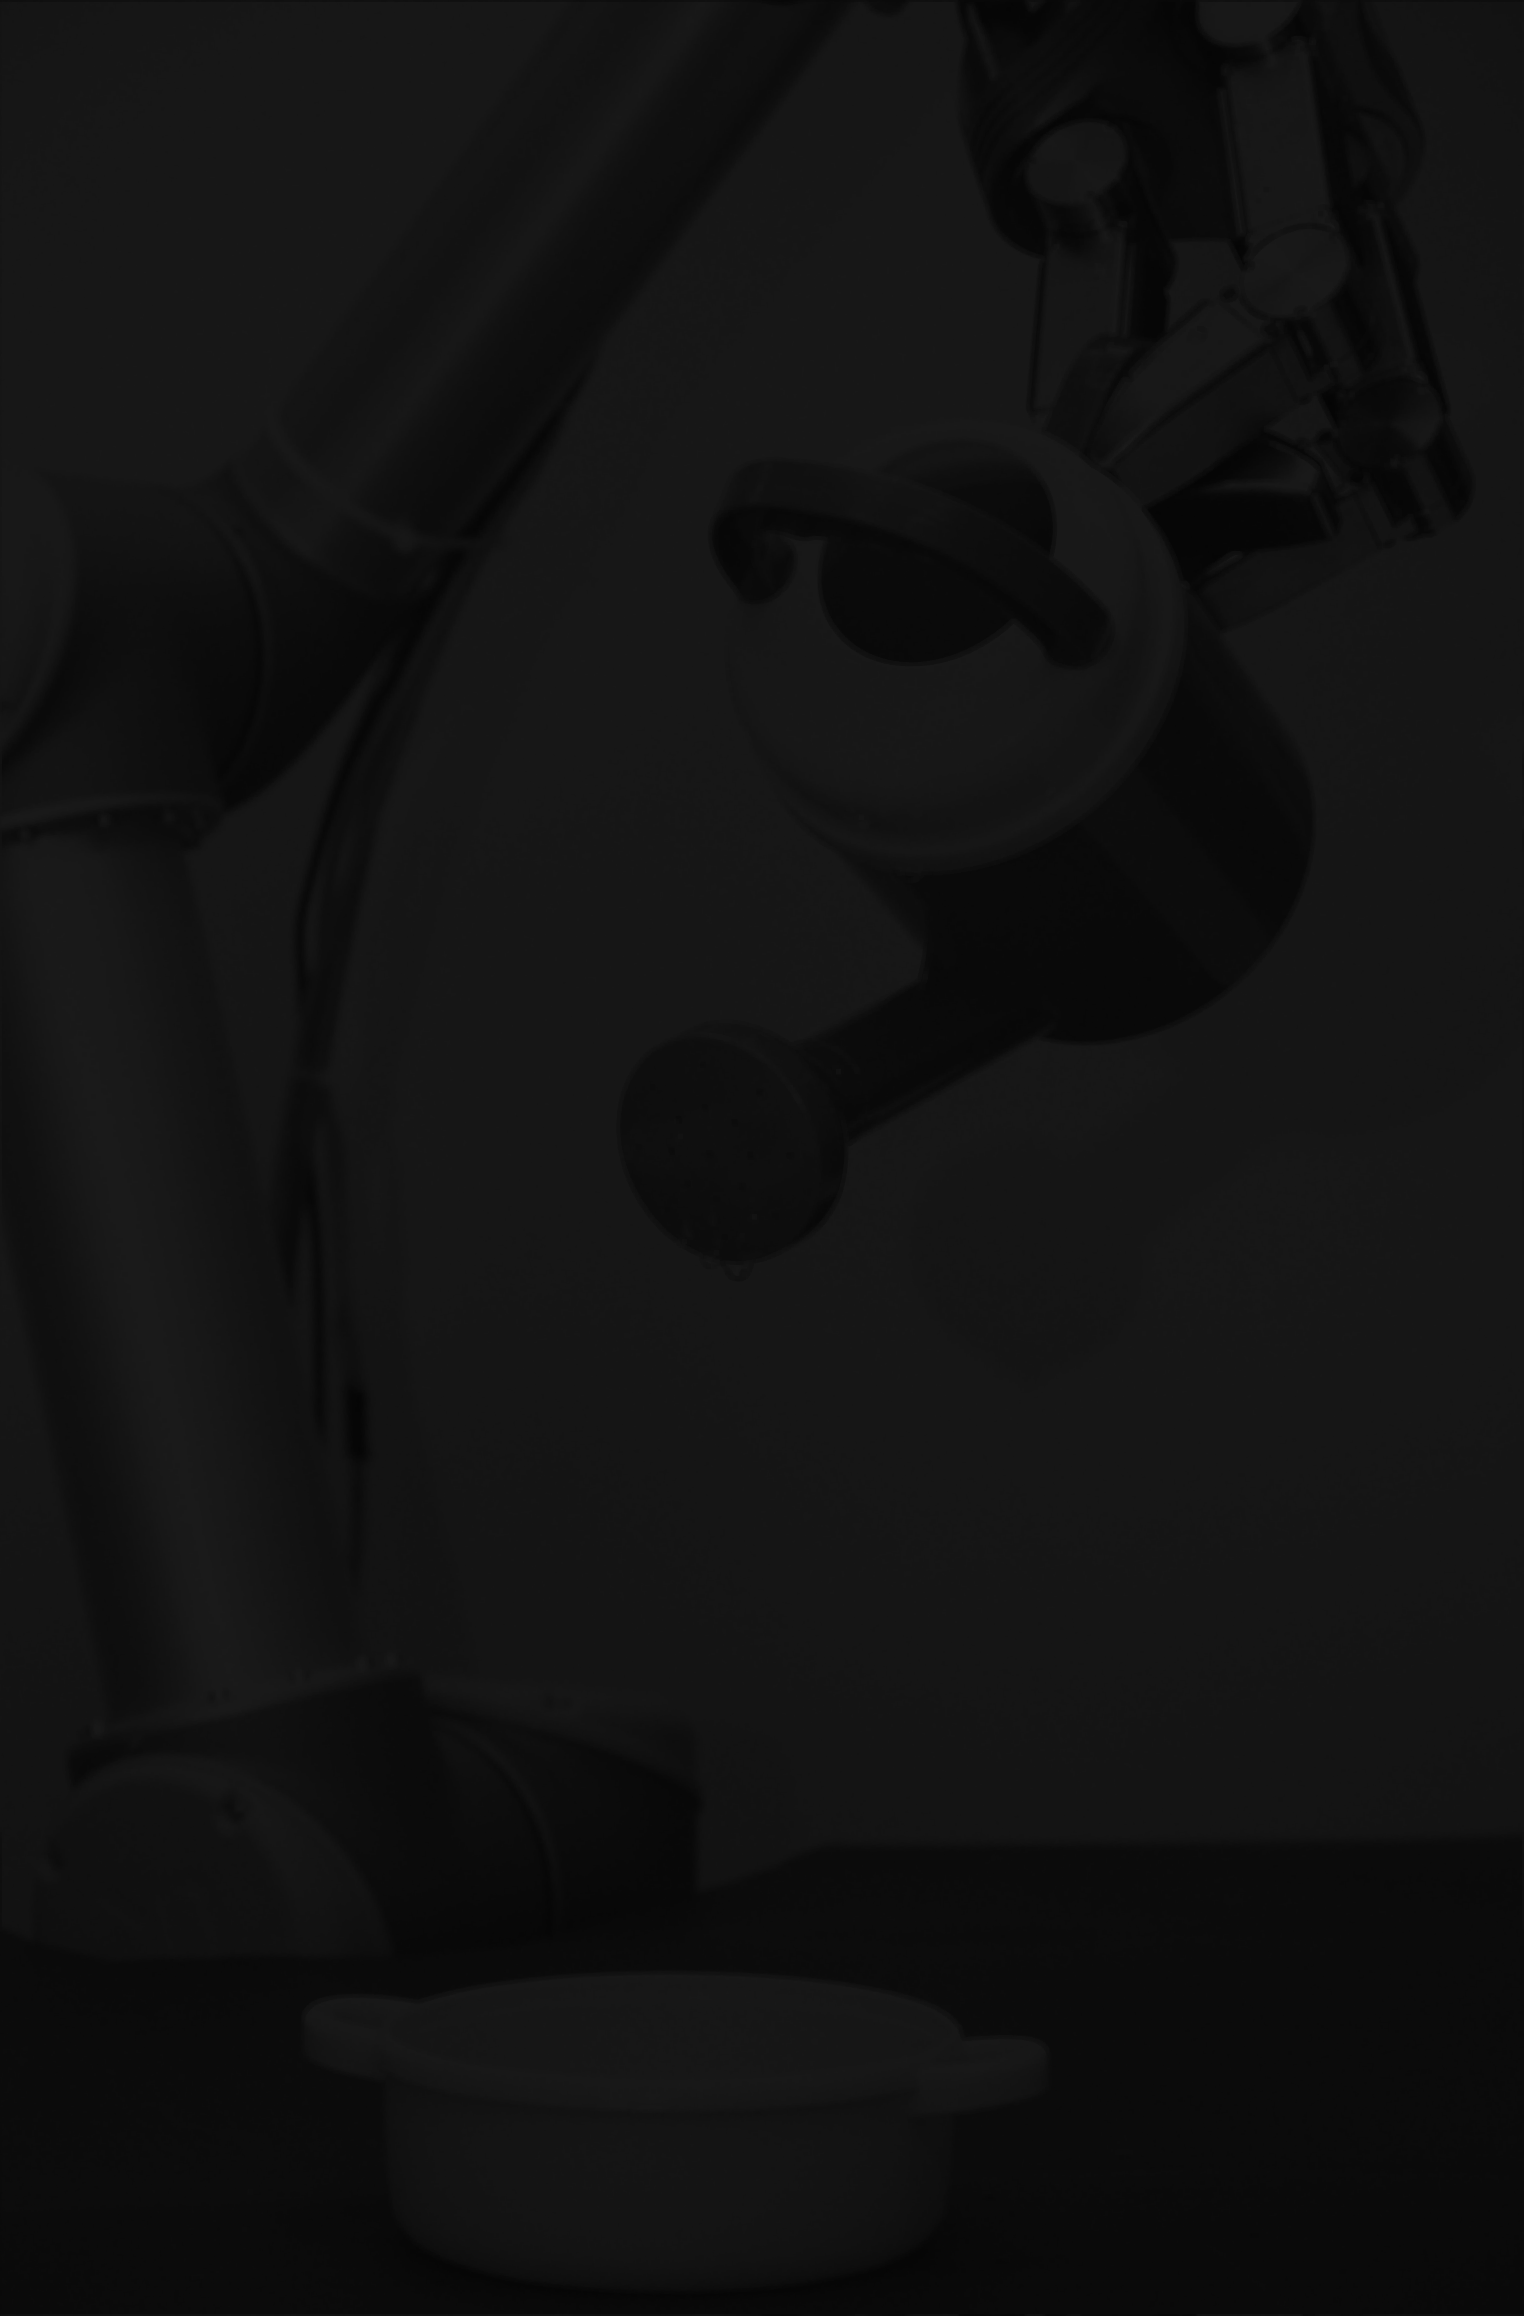
\includegraphics[width=\textwidth]{img3/test/contrast_5_0_1_final_img3.png}
    \end{subfigure}
    \begin{subfigure}[b]{0.1\textwidth}
        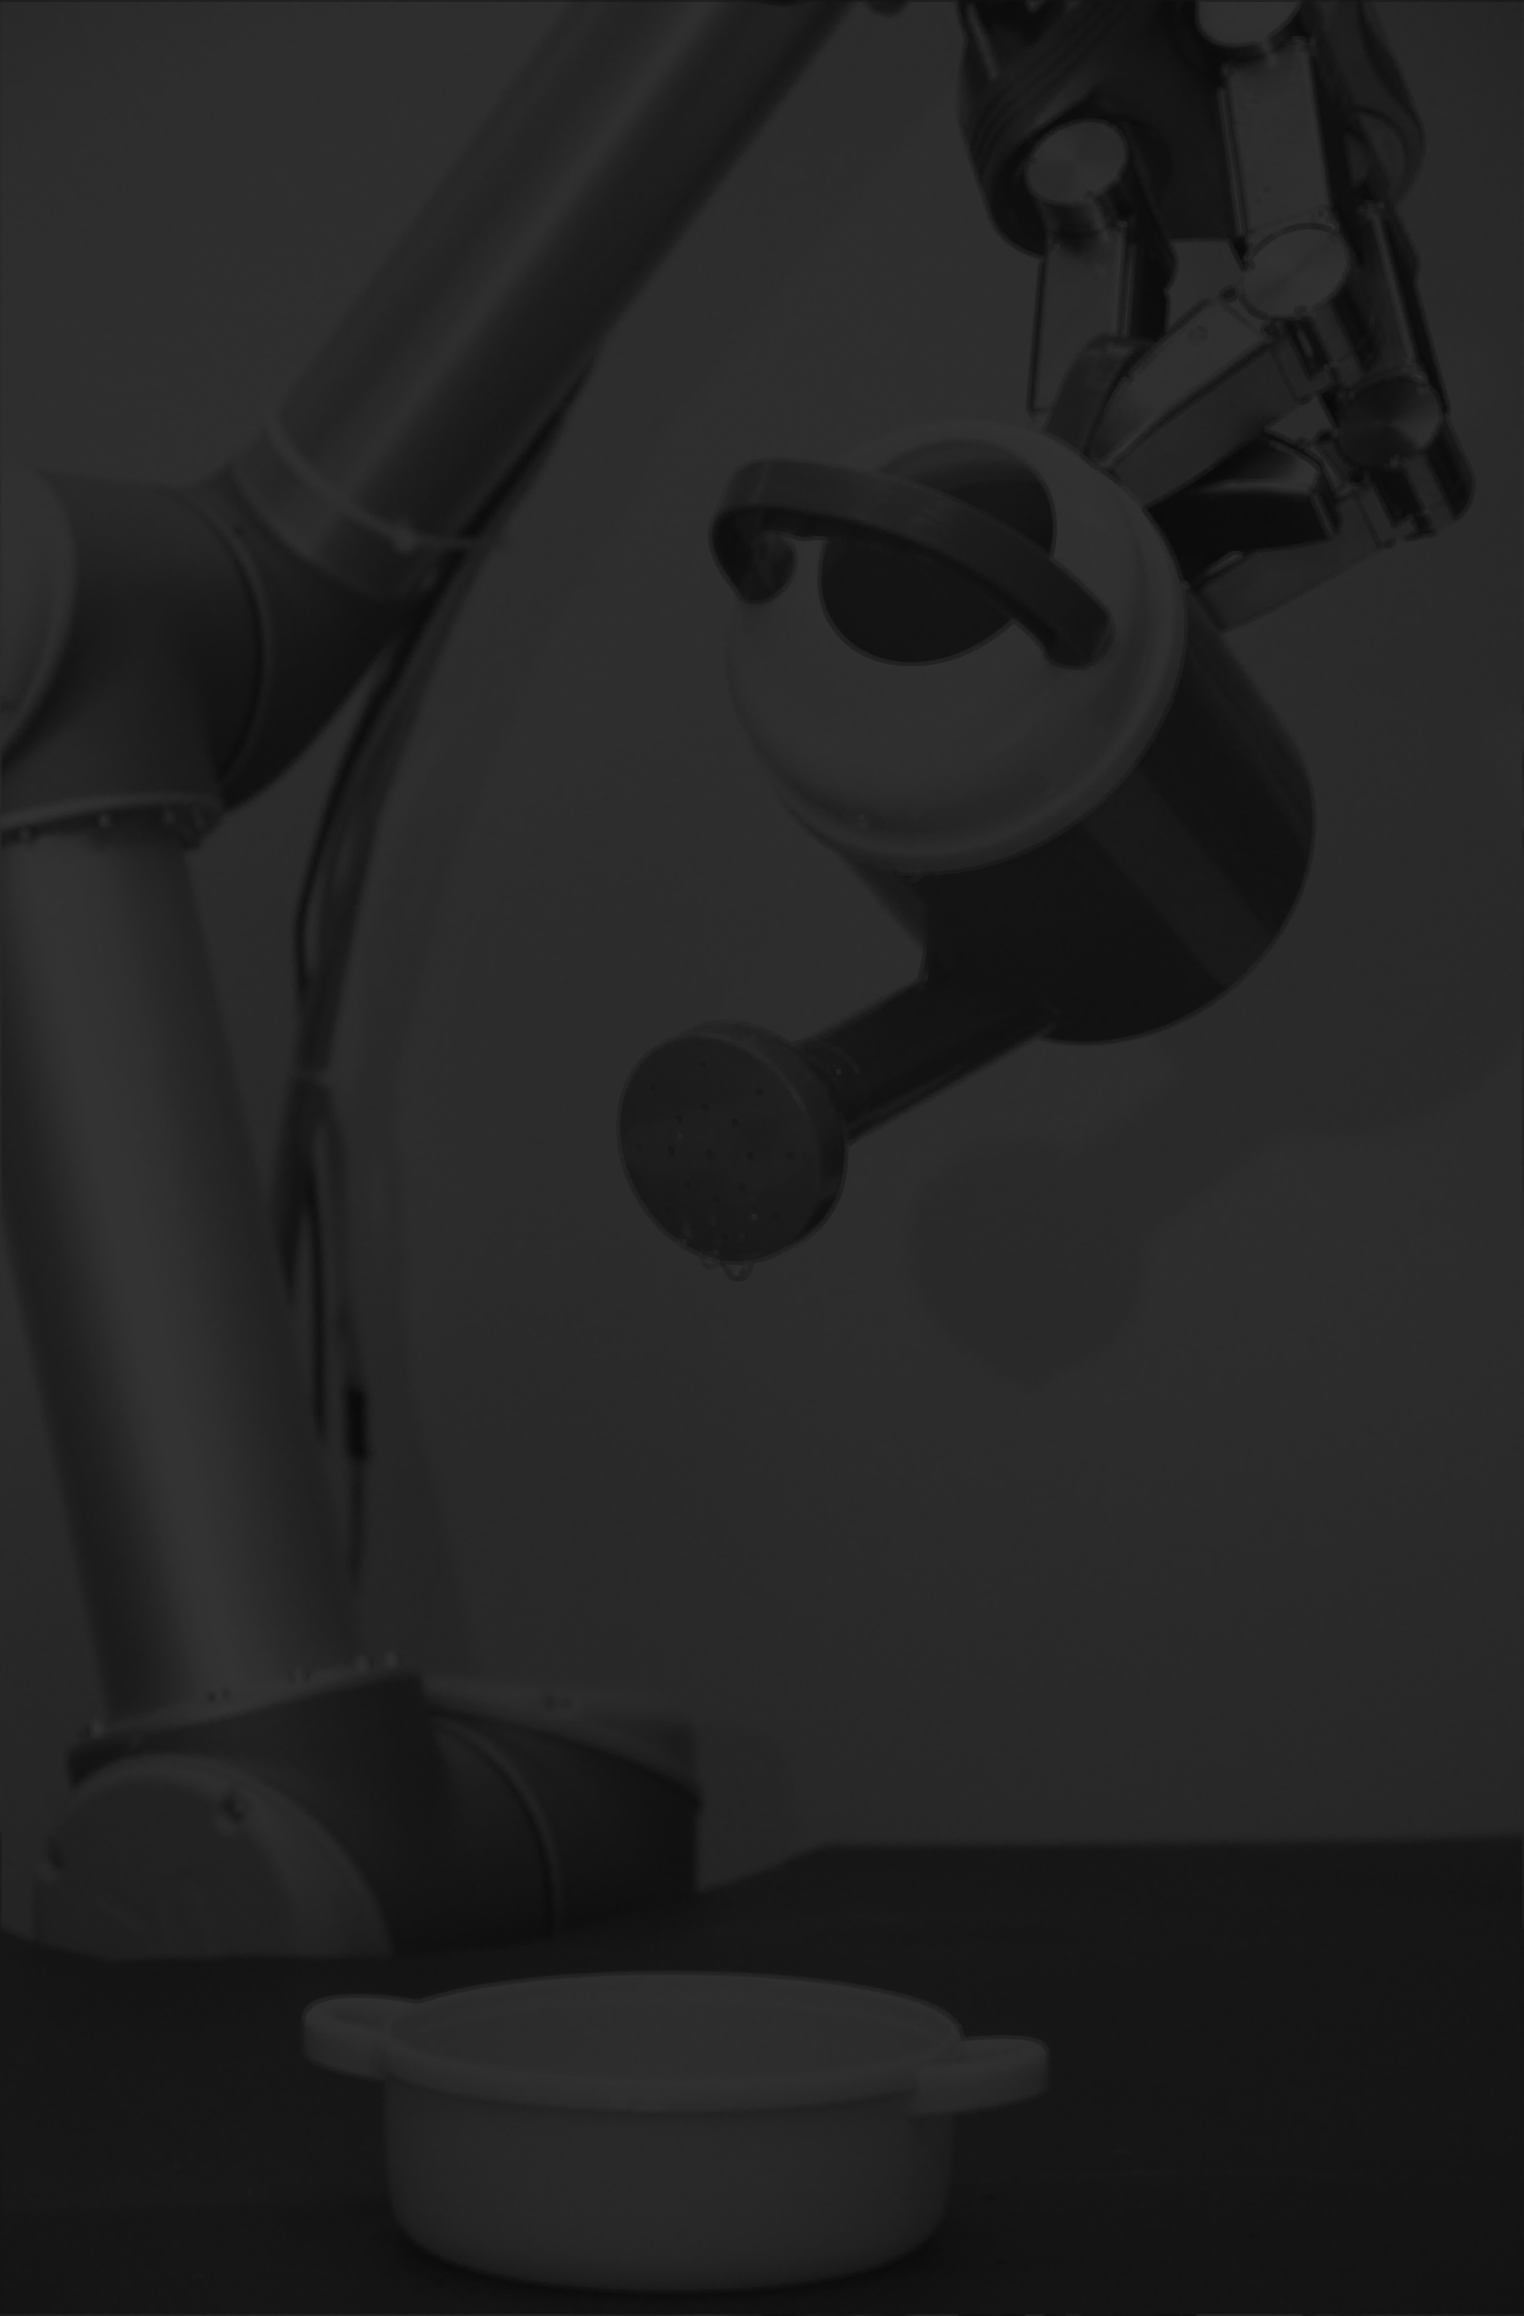
\includegraphics[width=\textwidth]{img3/test/contrast_5_0_2_final_img3.png}
    \end{subfigure}
    \begin{subfigure}[b]{0.1\textwidth}
        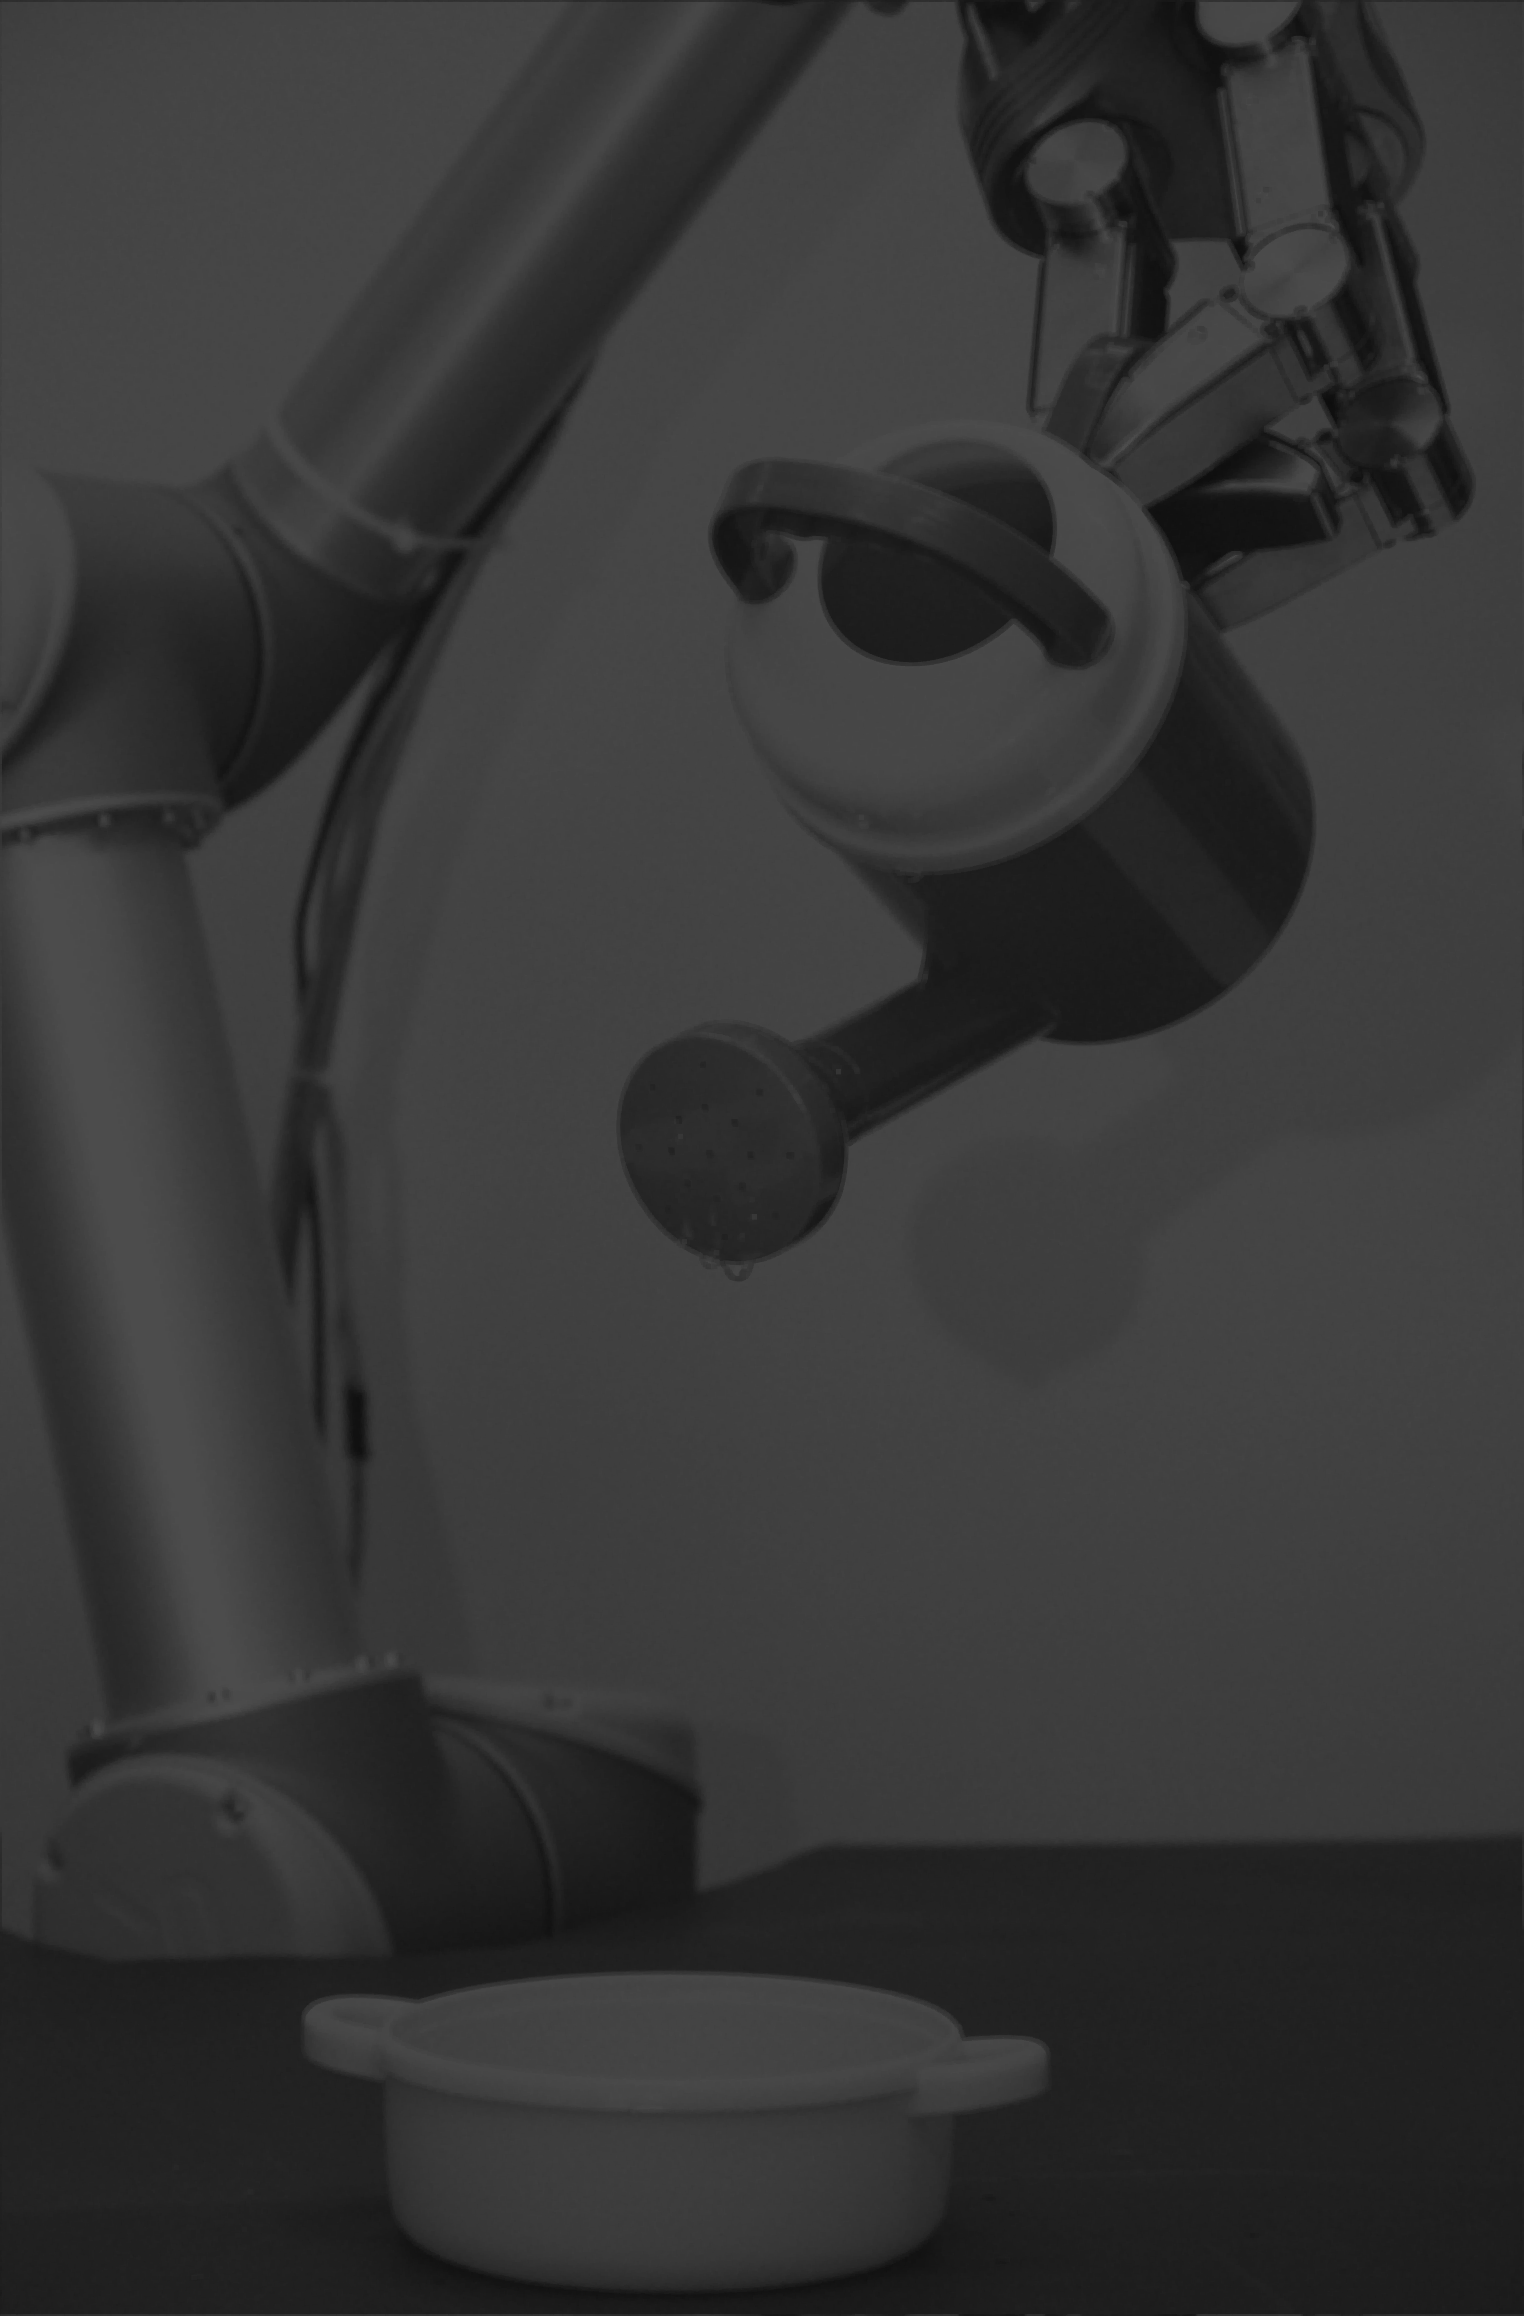
\includegraphics[width=\textwidth]{img3/test/contrast_5_0_3_final_img3.png}
    \end{subfigure}
    \begin{subfigure}[b]{0.1\textwidth}
        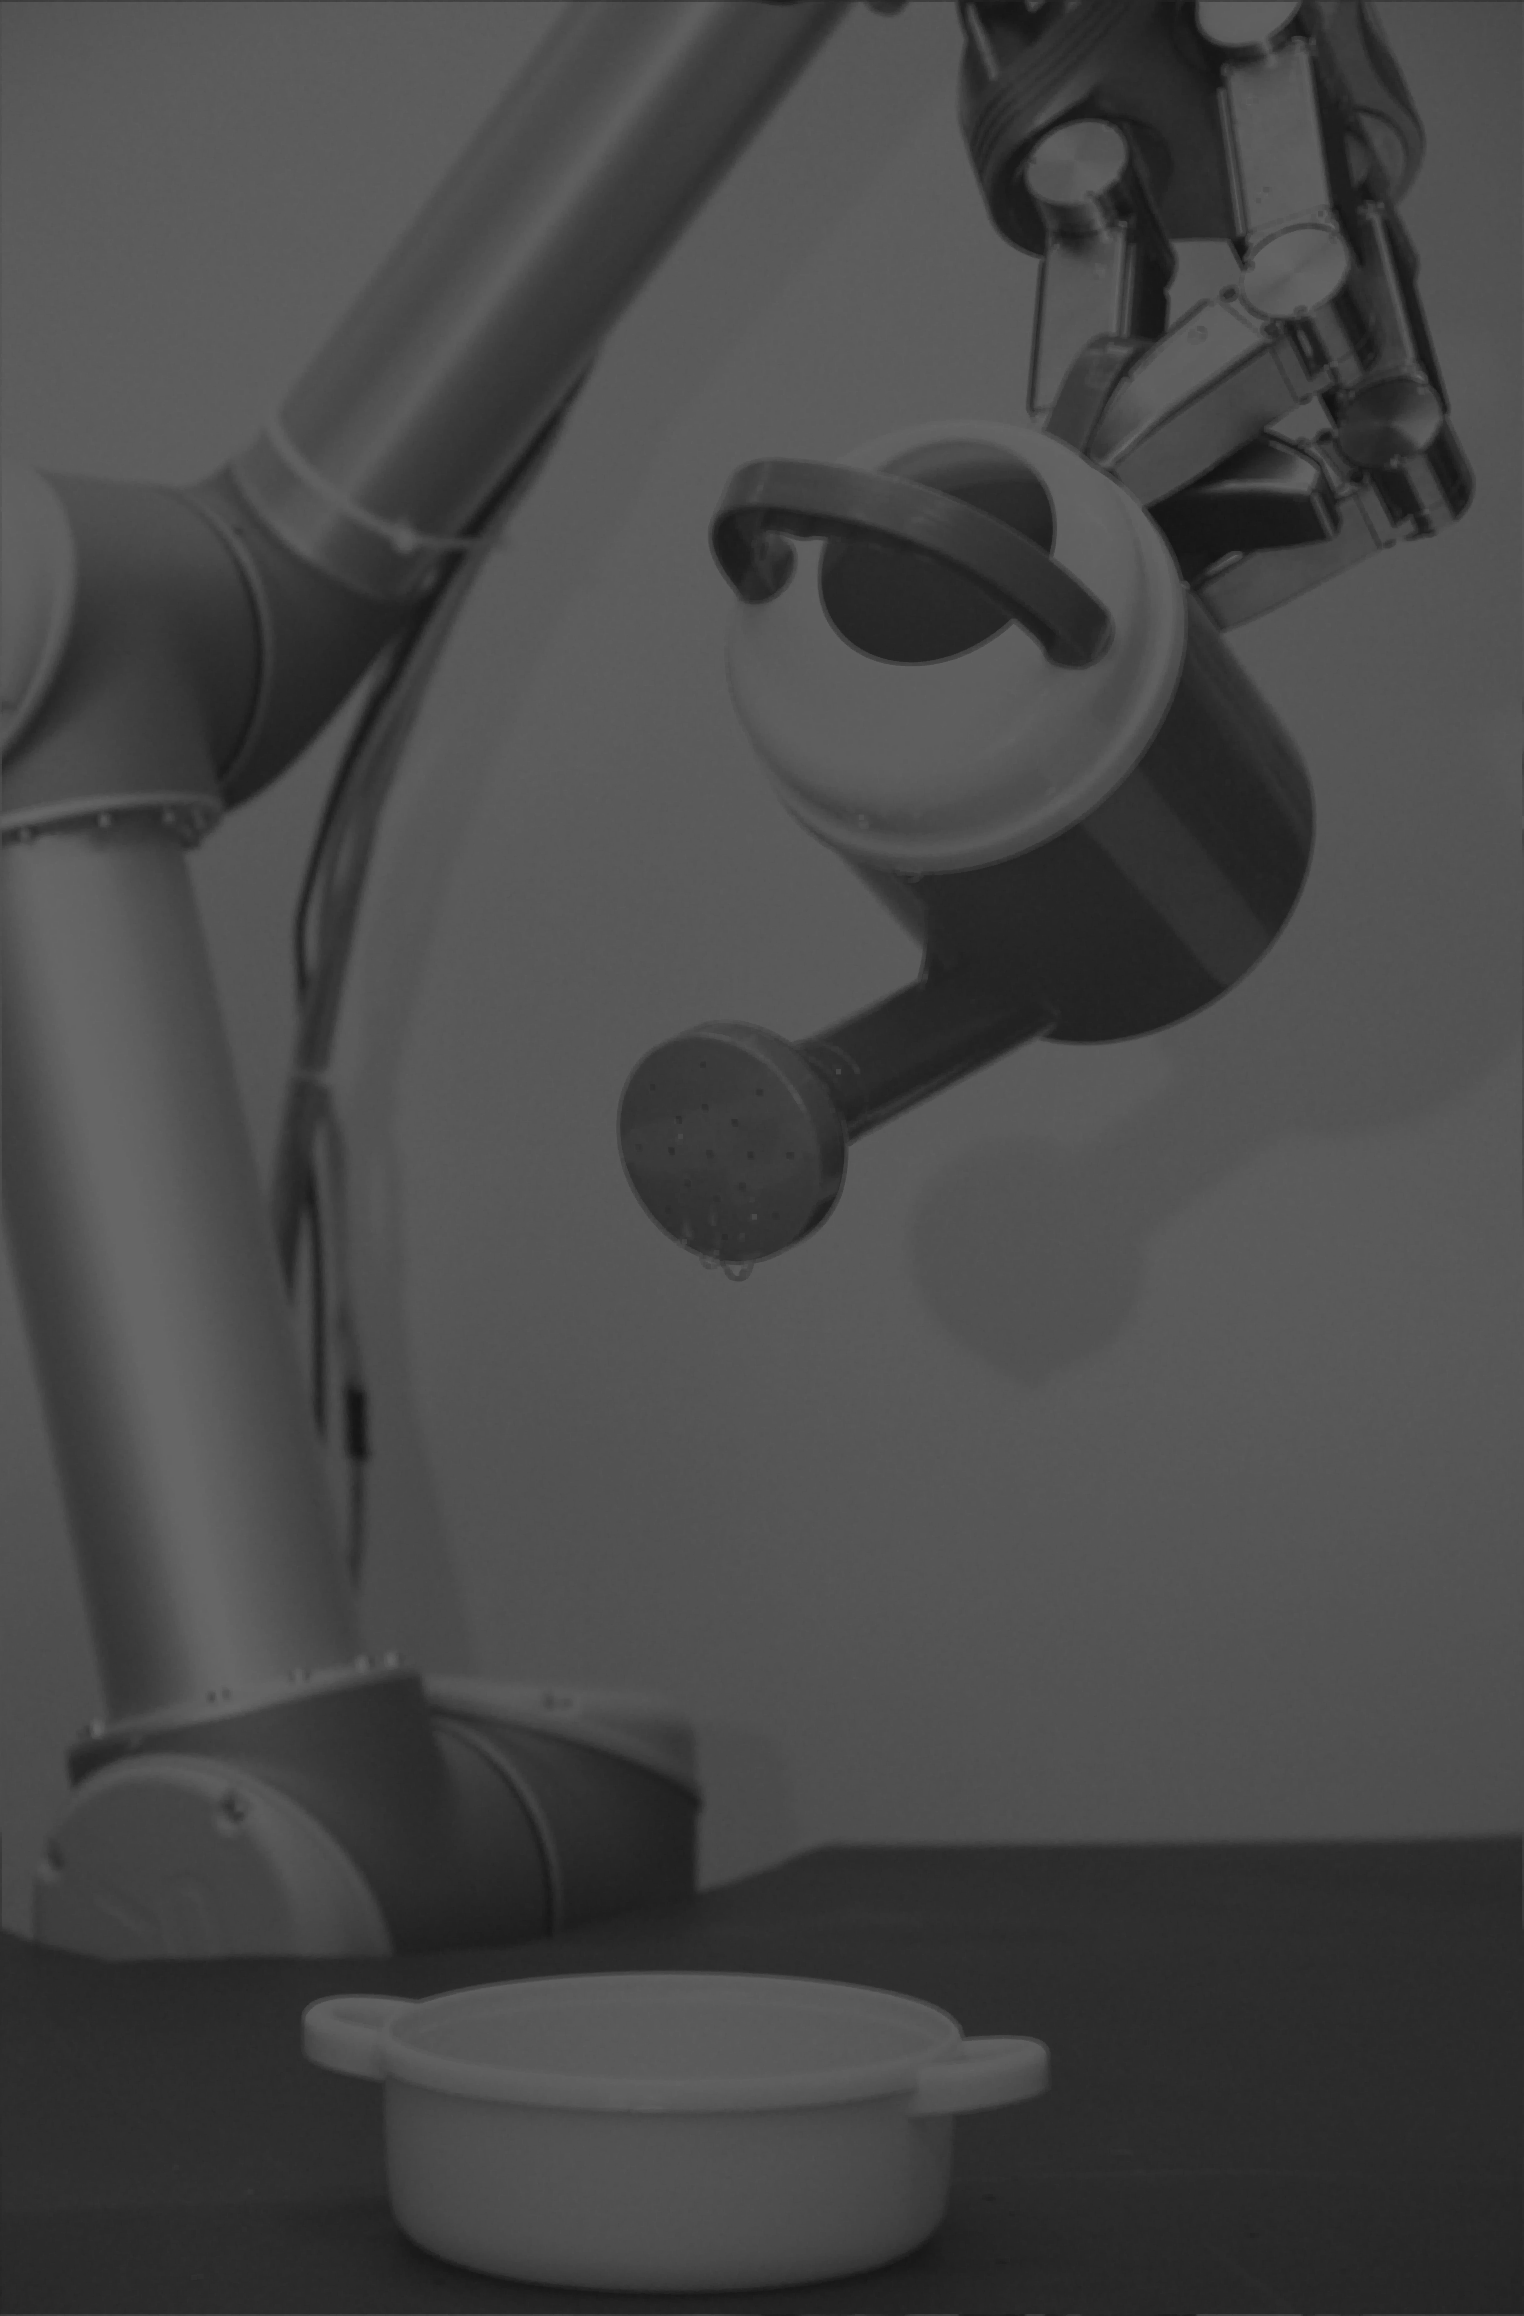
\includegraphics[width=\textwidth]{img3/test/contrast_5_0_4_final_img3.png}
    \end{subfigure}
    \begin{subfigure}[b]{0.1\textwidth}
        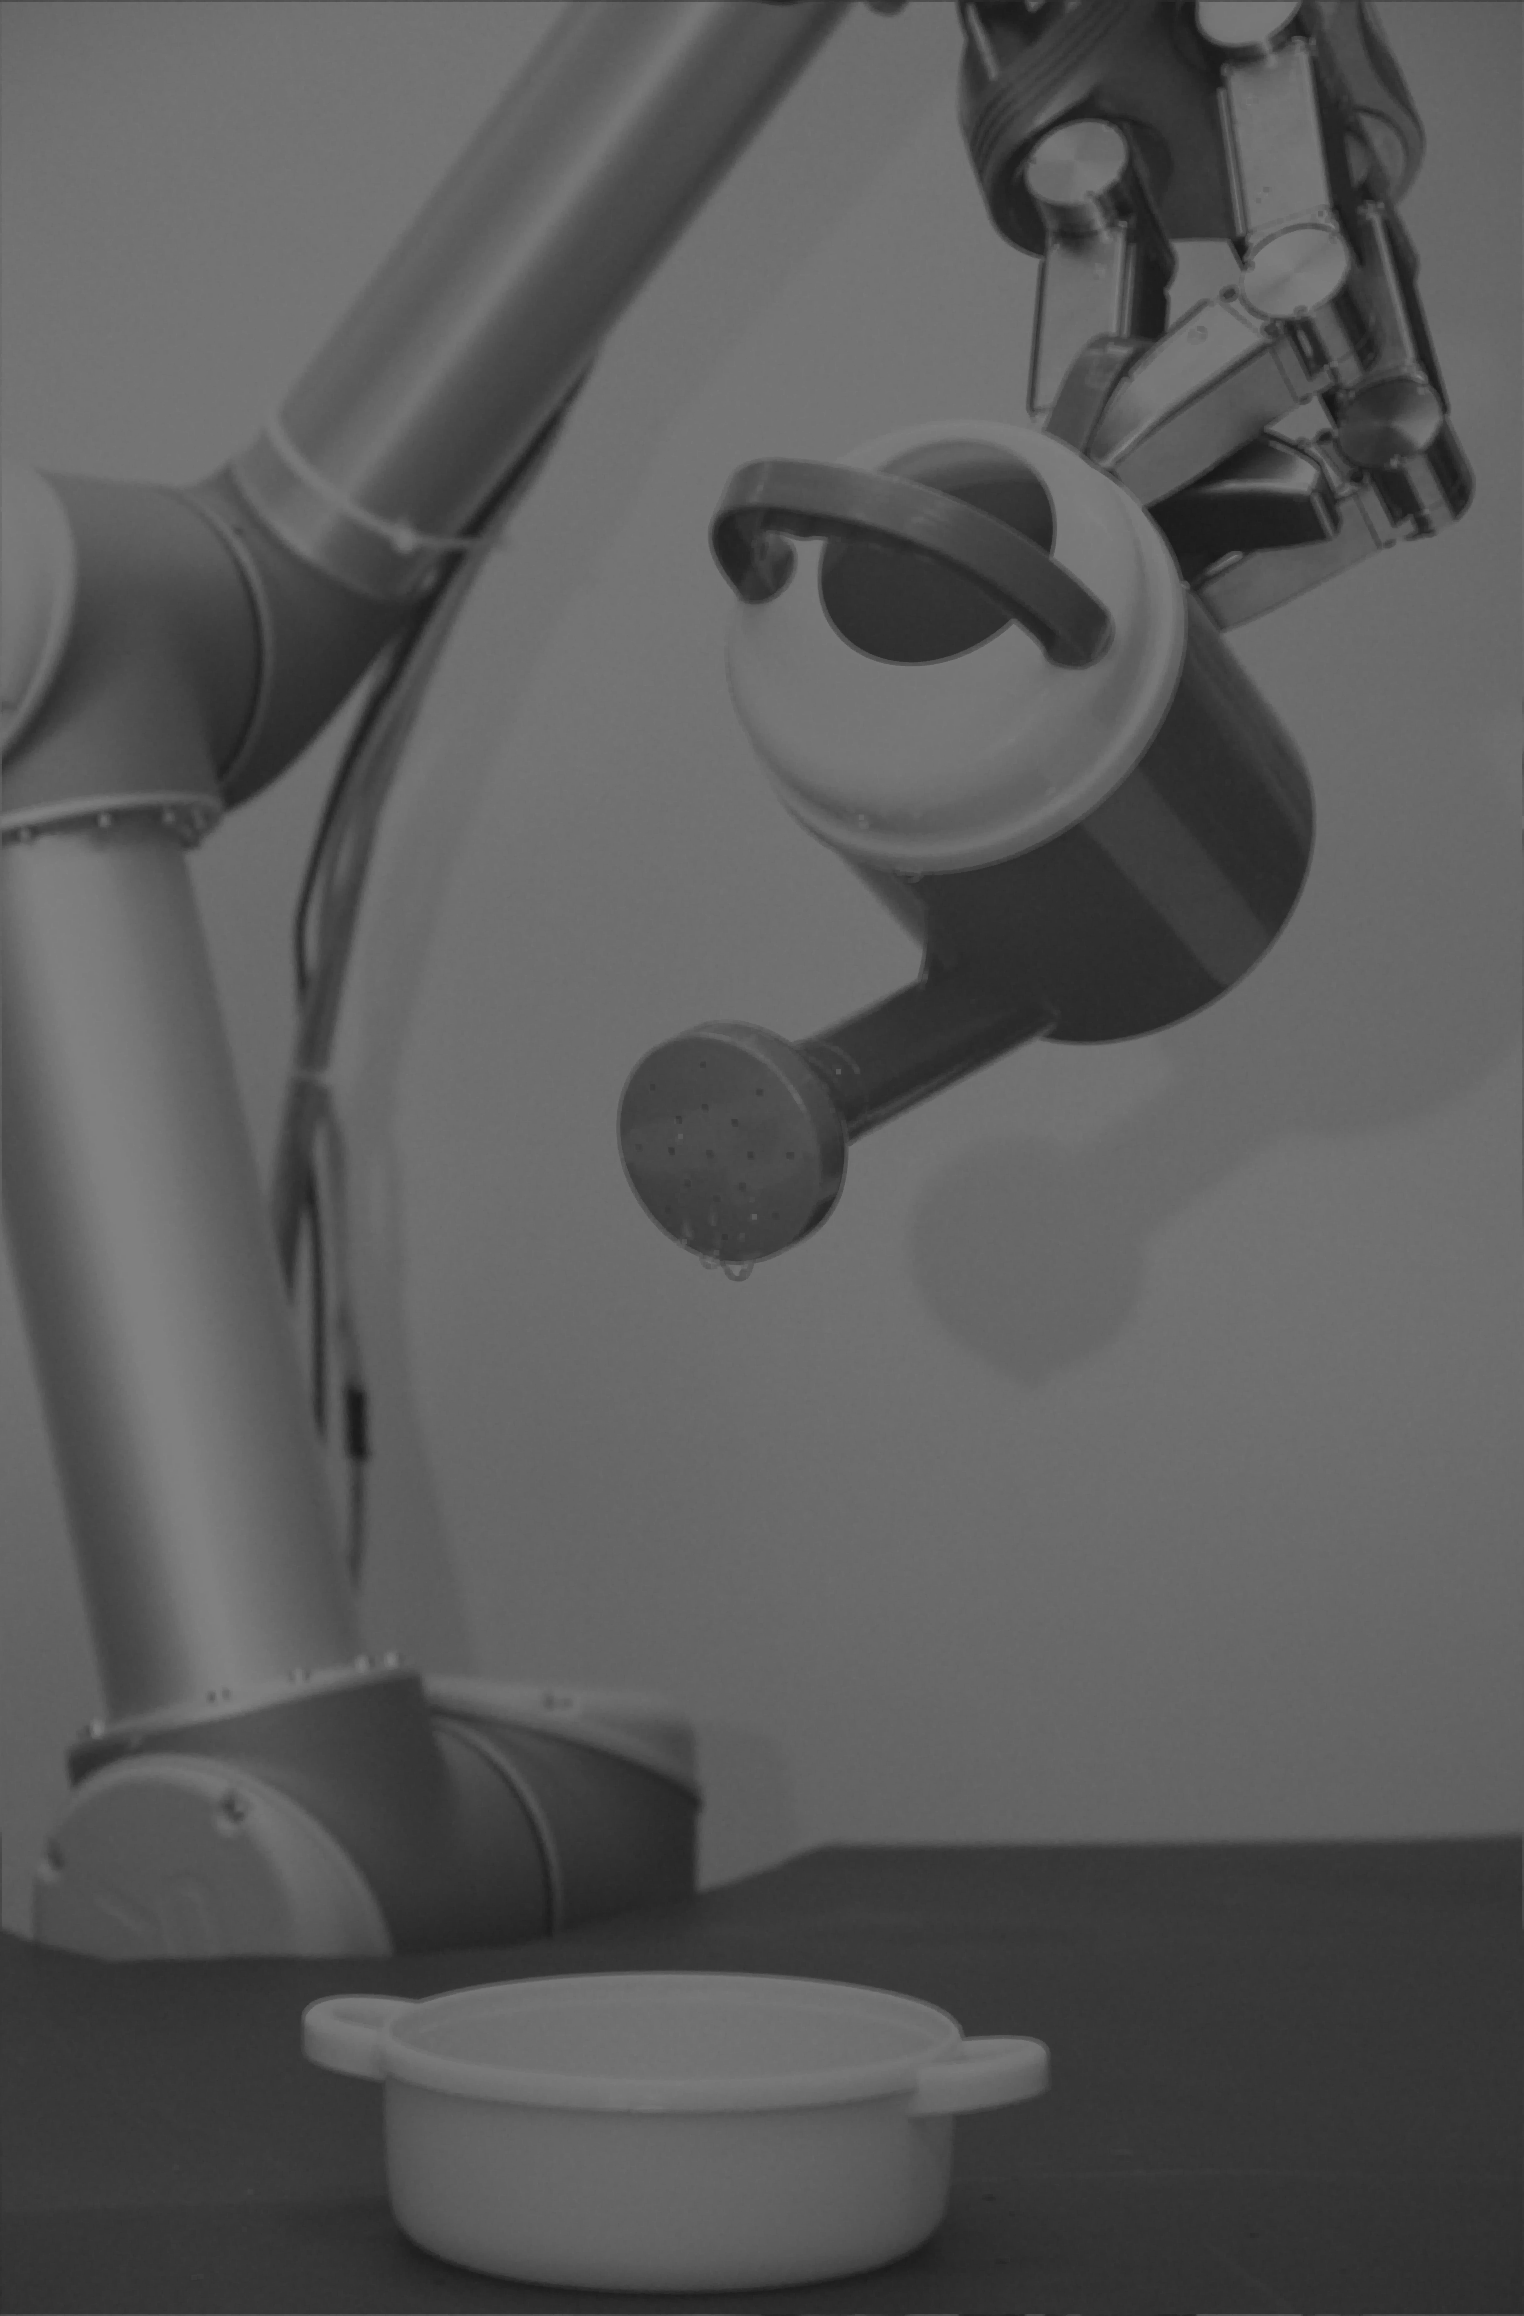
\includegraphics[width=\textwidth]{img3/test/contrast_5_0_5_final_img3.png}
    \end{subfigure}
    \begin{subfigure}[b]{0.1\textwidth}
        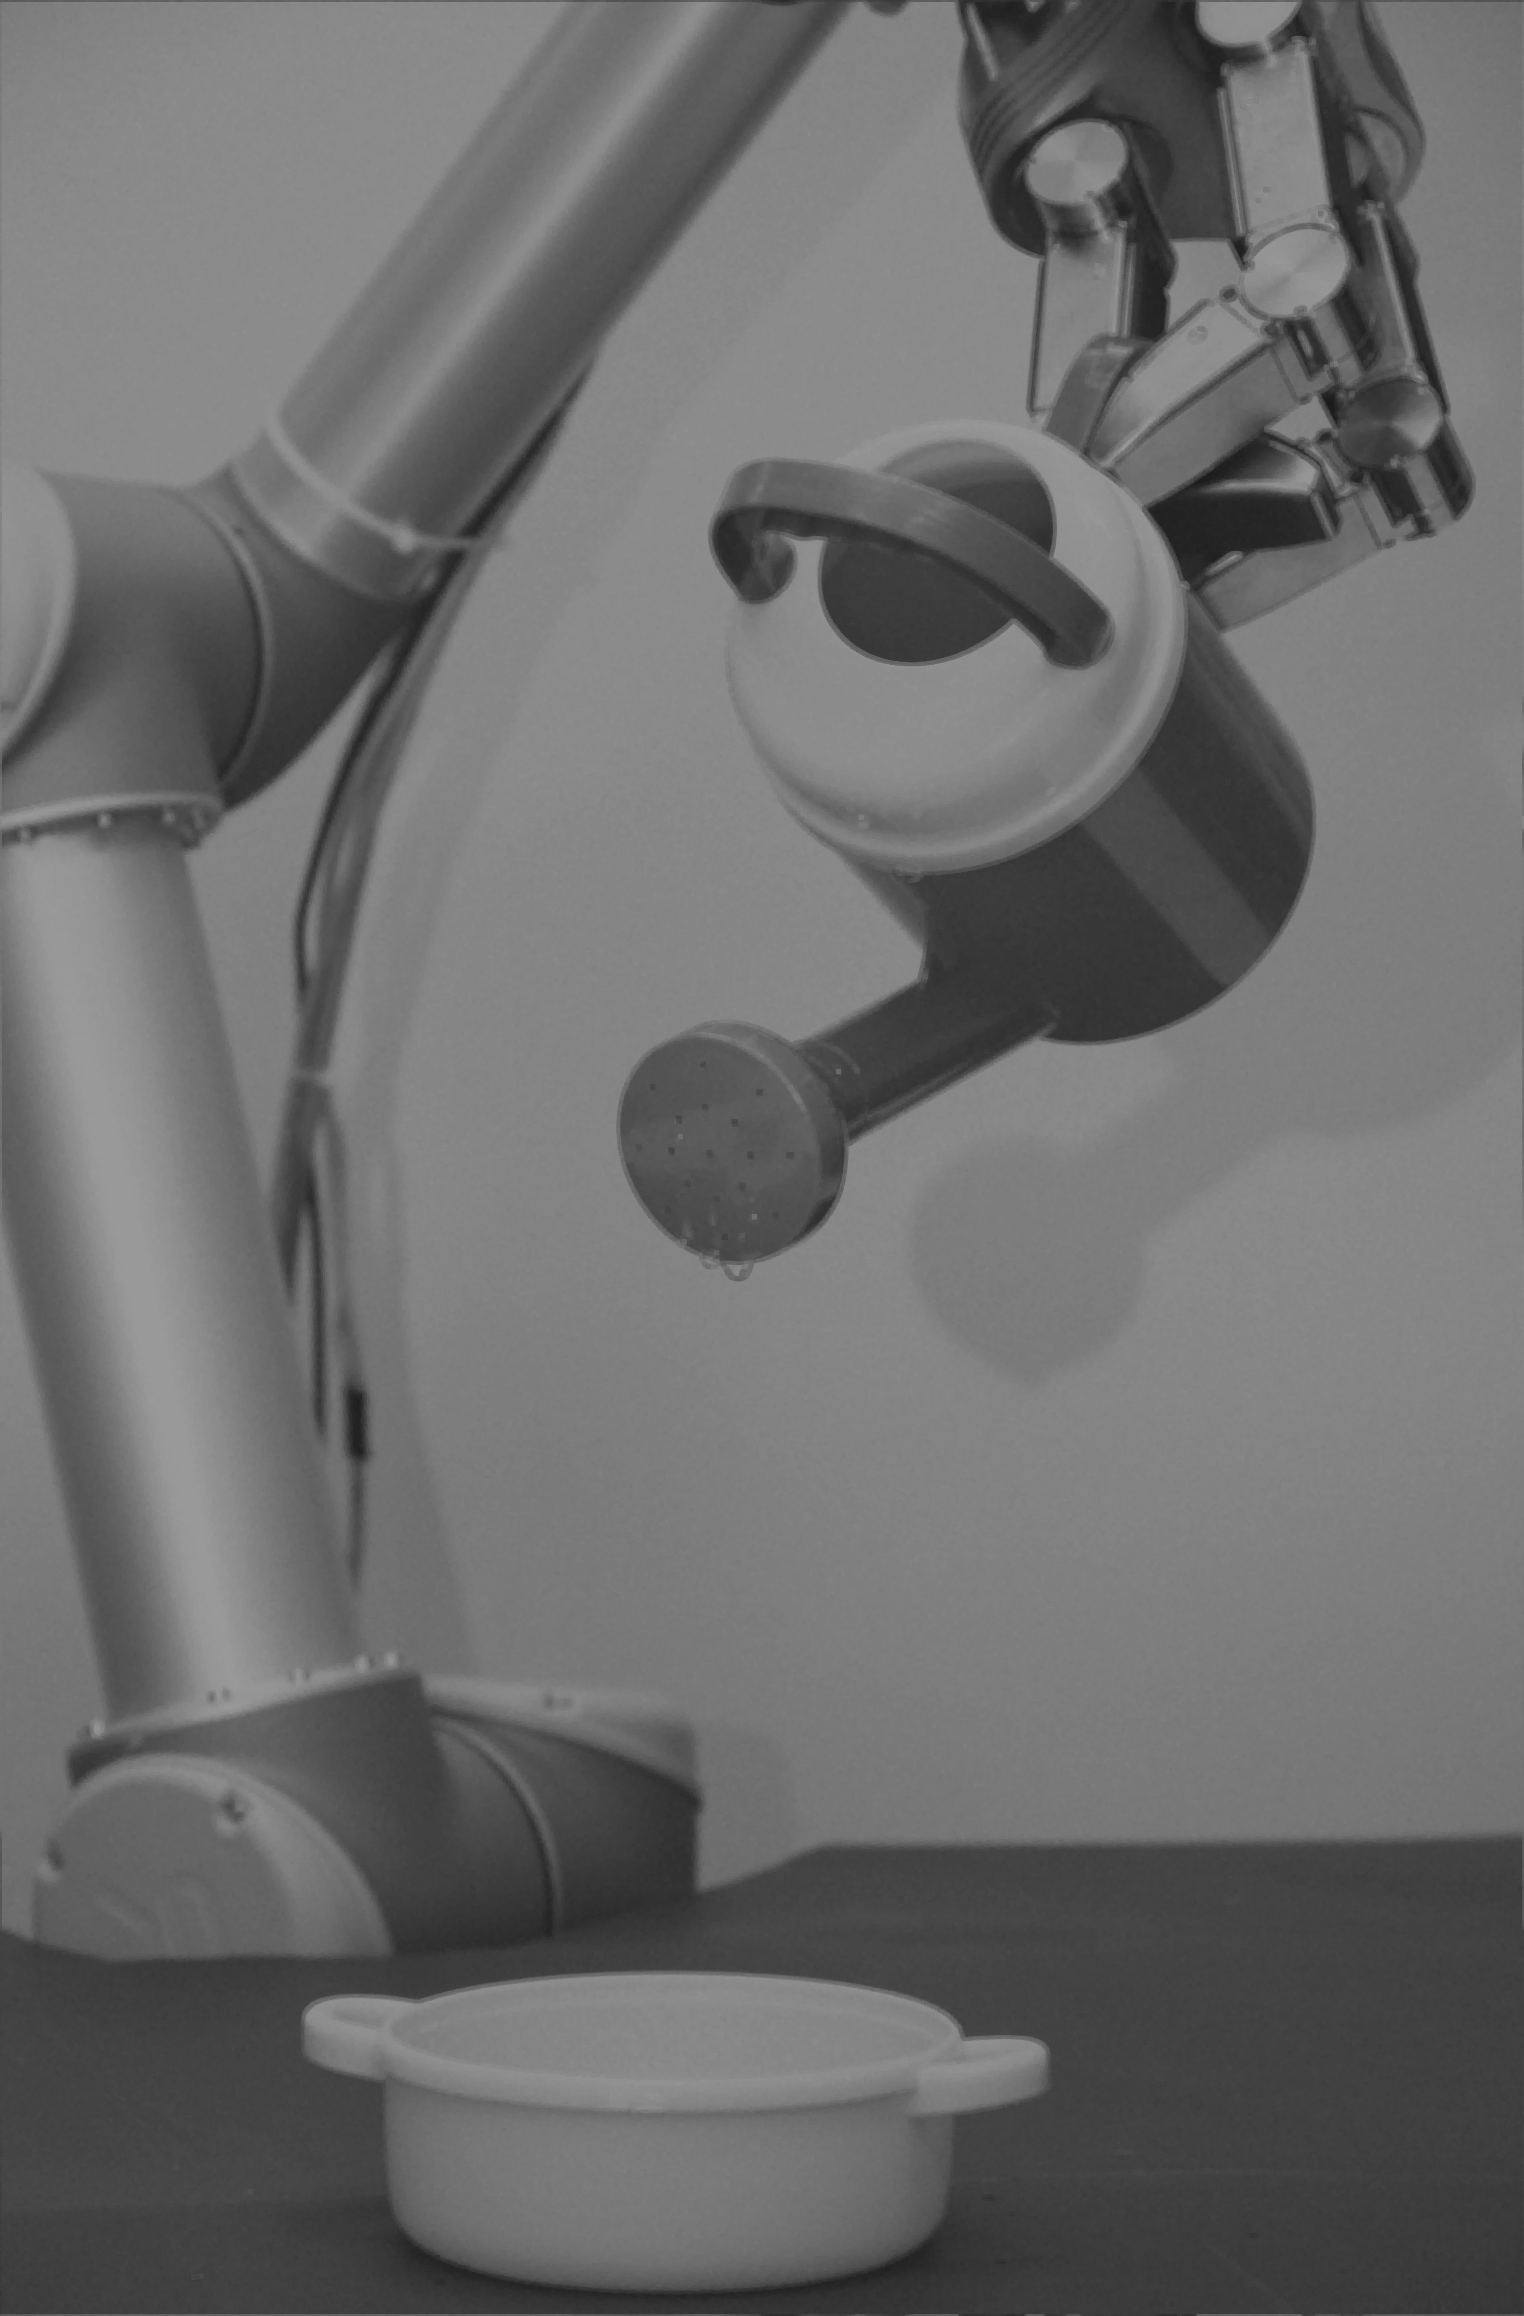
\includegraphics[width=\textwidth]{img3/test/contrast_5_0_6_final_img3.png}
    \end{subfigure}
    \begin{subfigure}[b]{0.1\textwidth}
        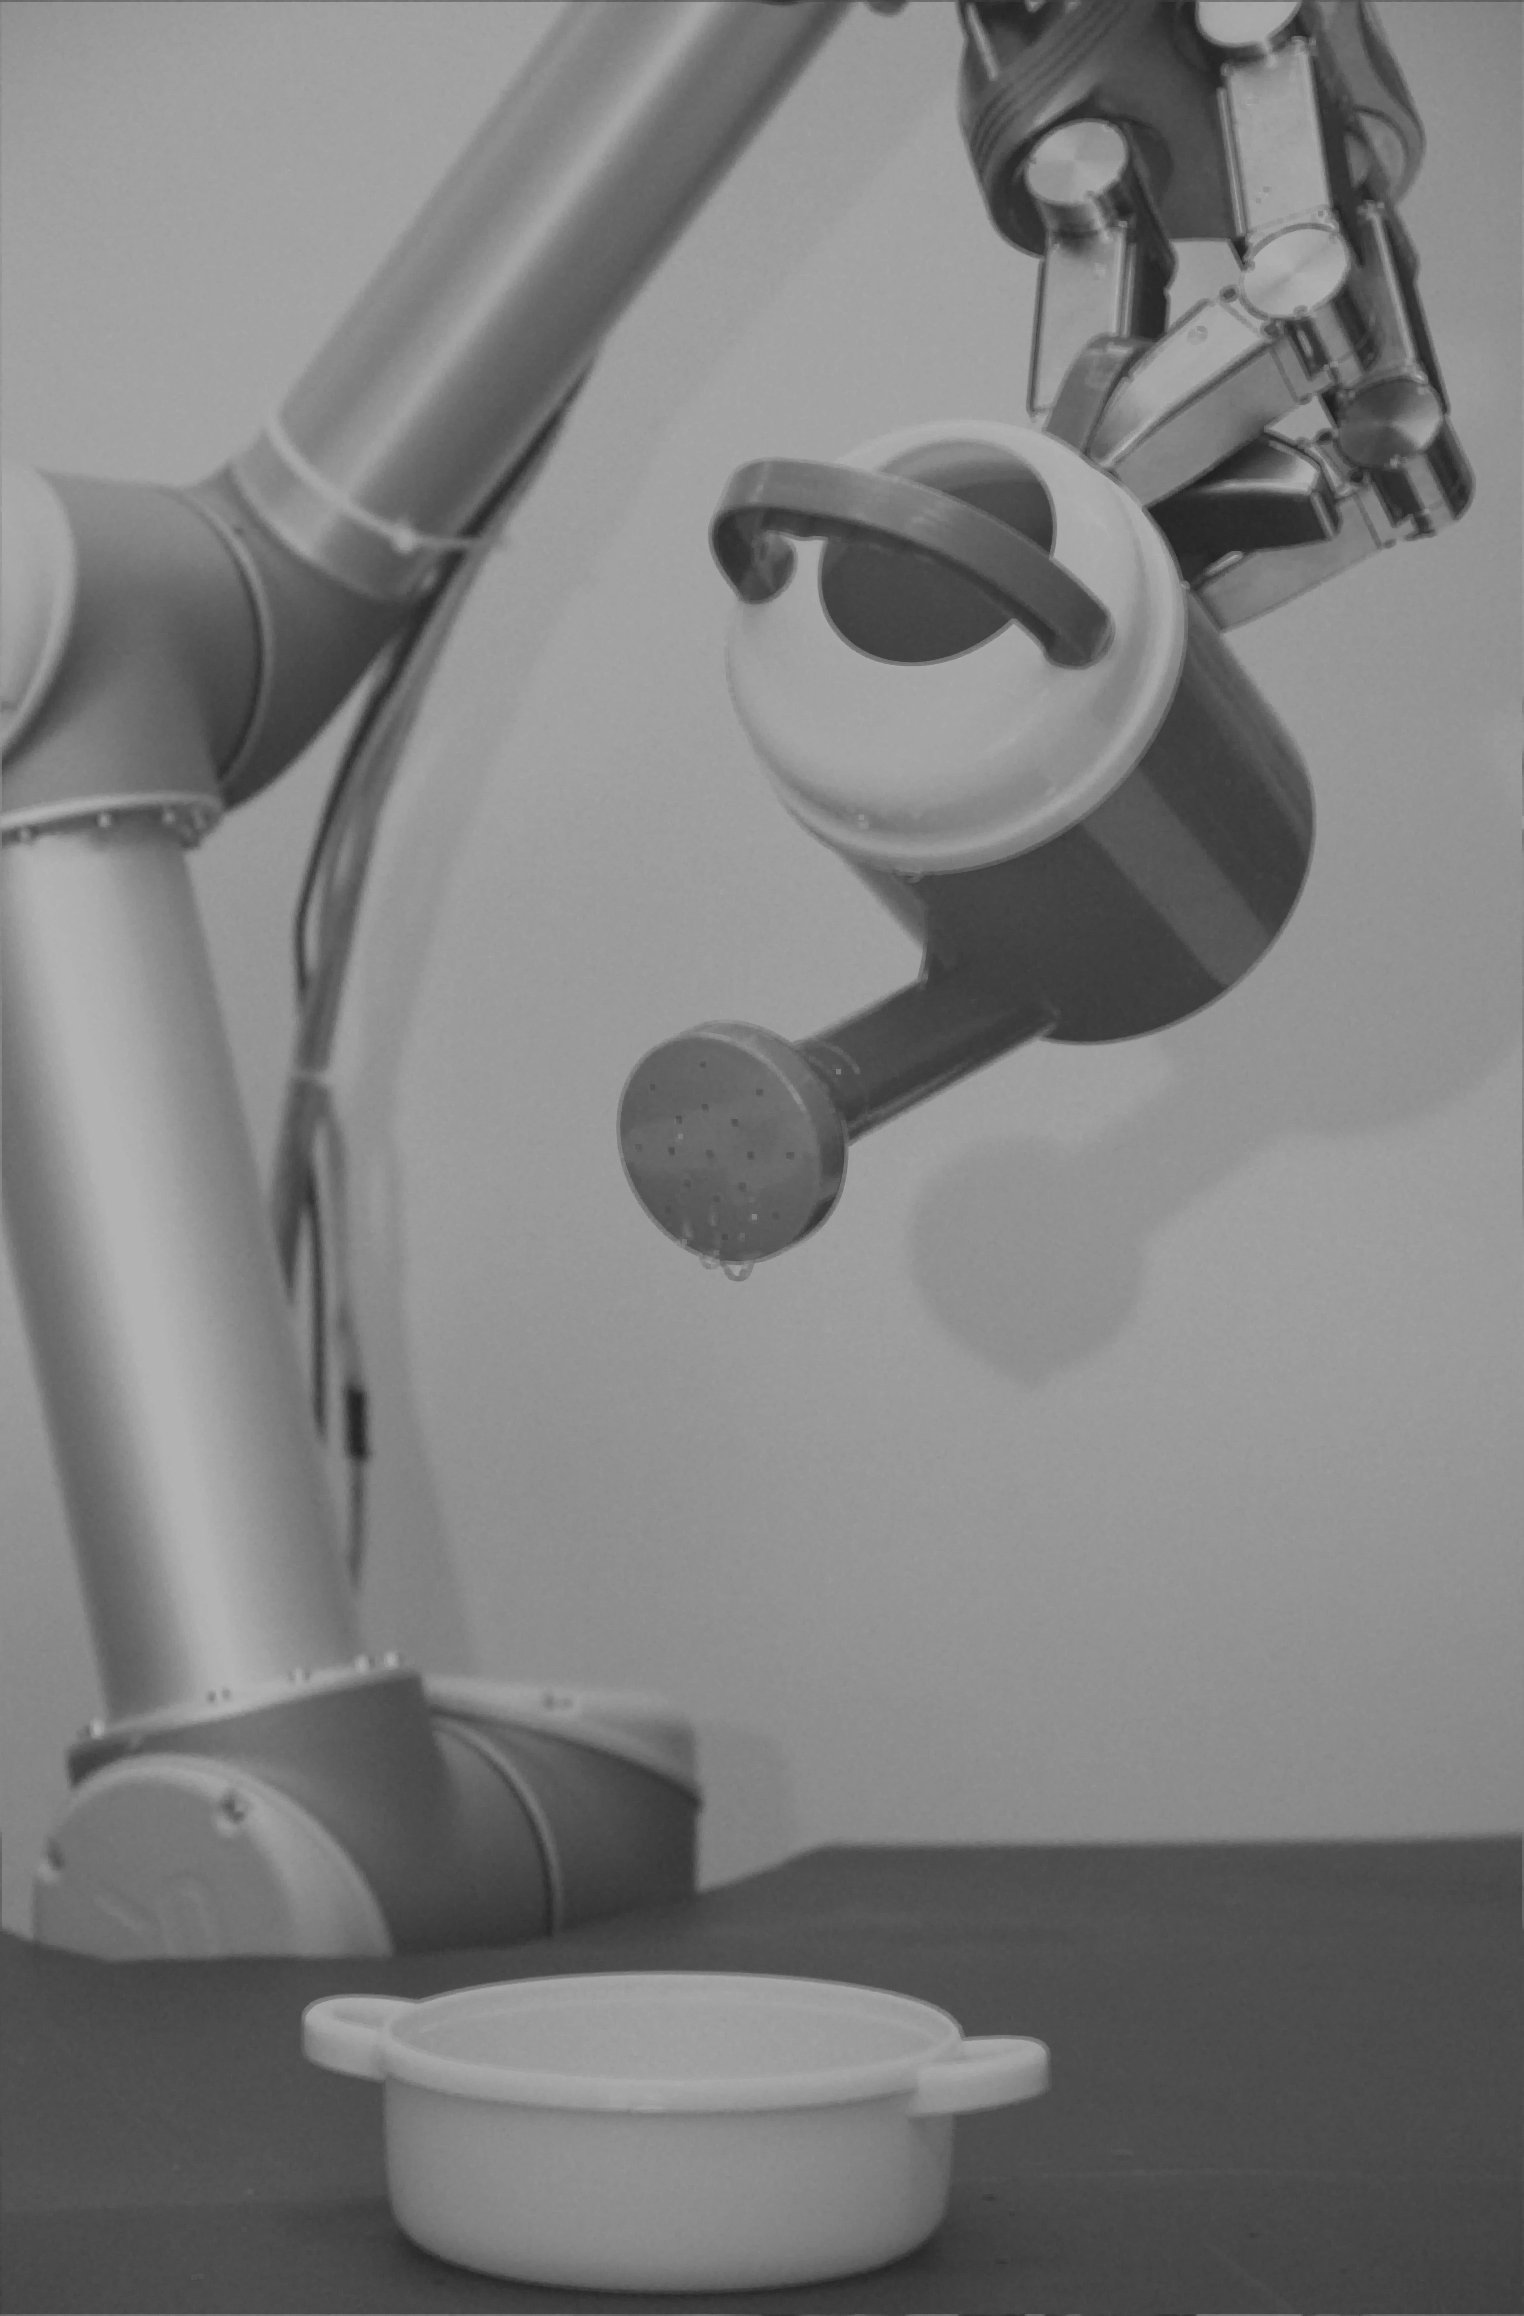
\includegraphics[width=\textwidth]{img3/test/contrast_5_0_7_final_img3.png}
    \end{subfigure}
    \begin{subfigure}[b]{0.1\textwidth}
        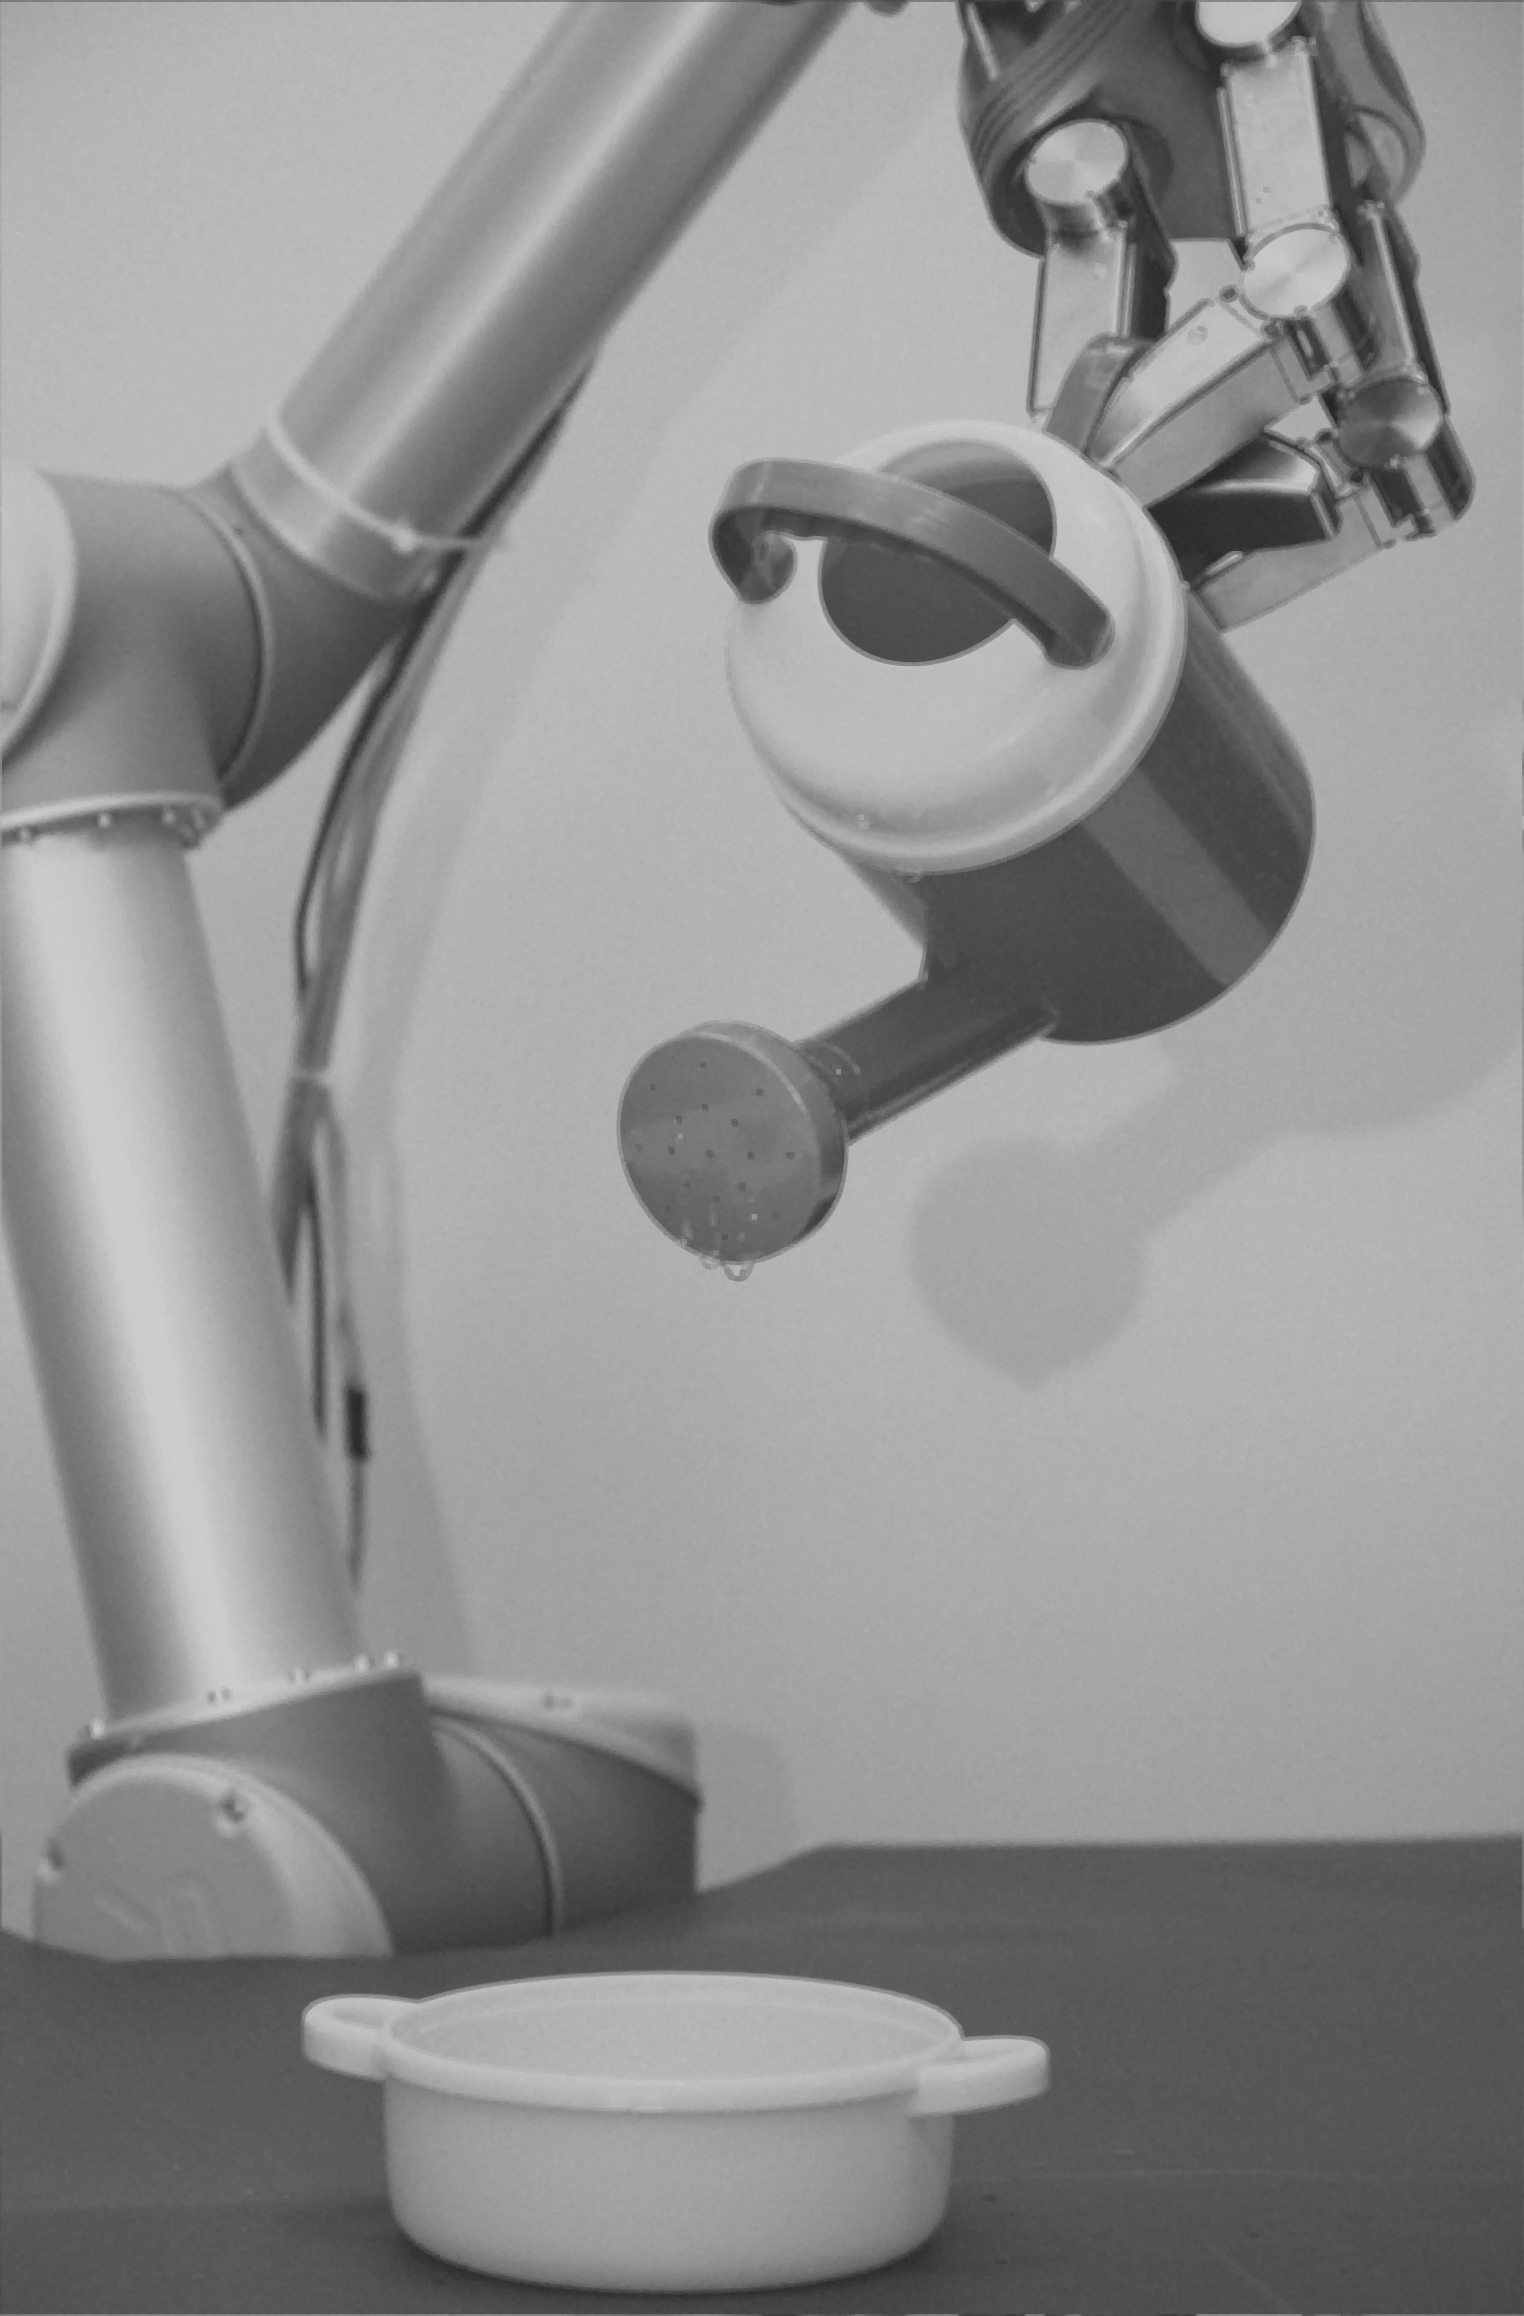
\includegraphics[width=\textwidth]{img3/test/contrast_5_0_8_final_img3.png}
    \end{subfigure}
    \begin{subfigure}[b]{0.1\textwidth}
        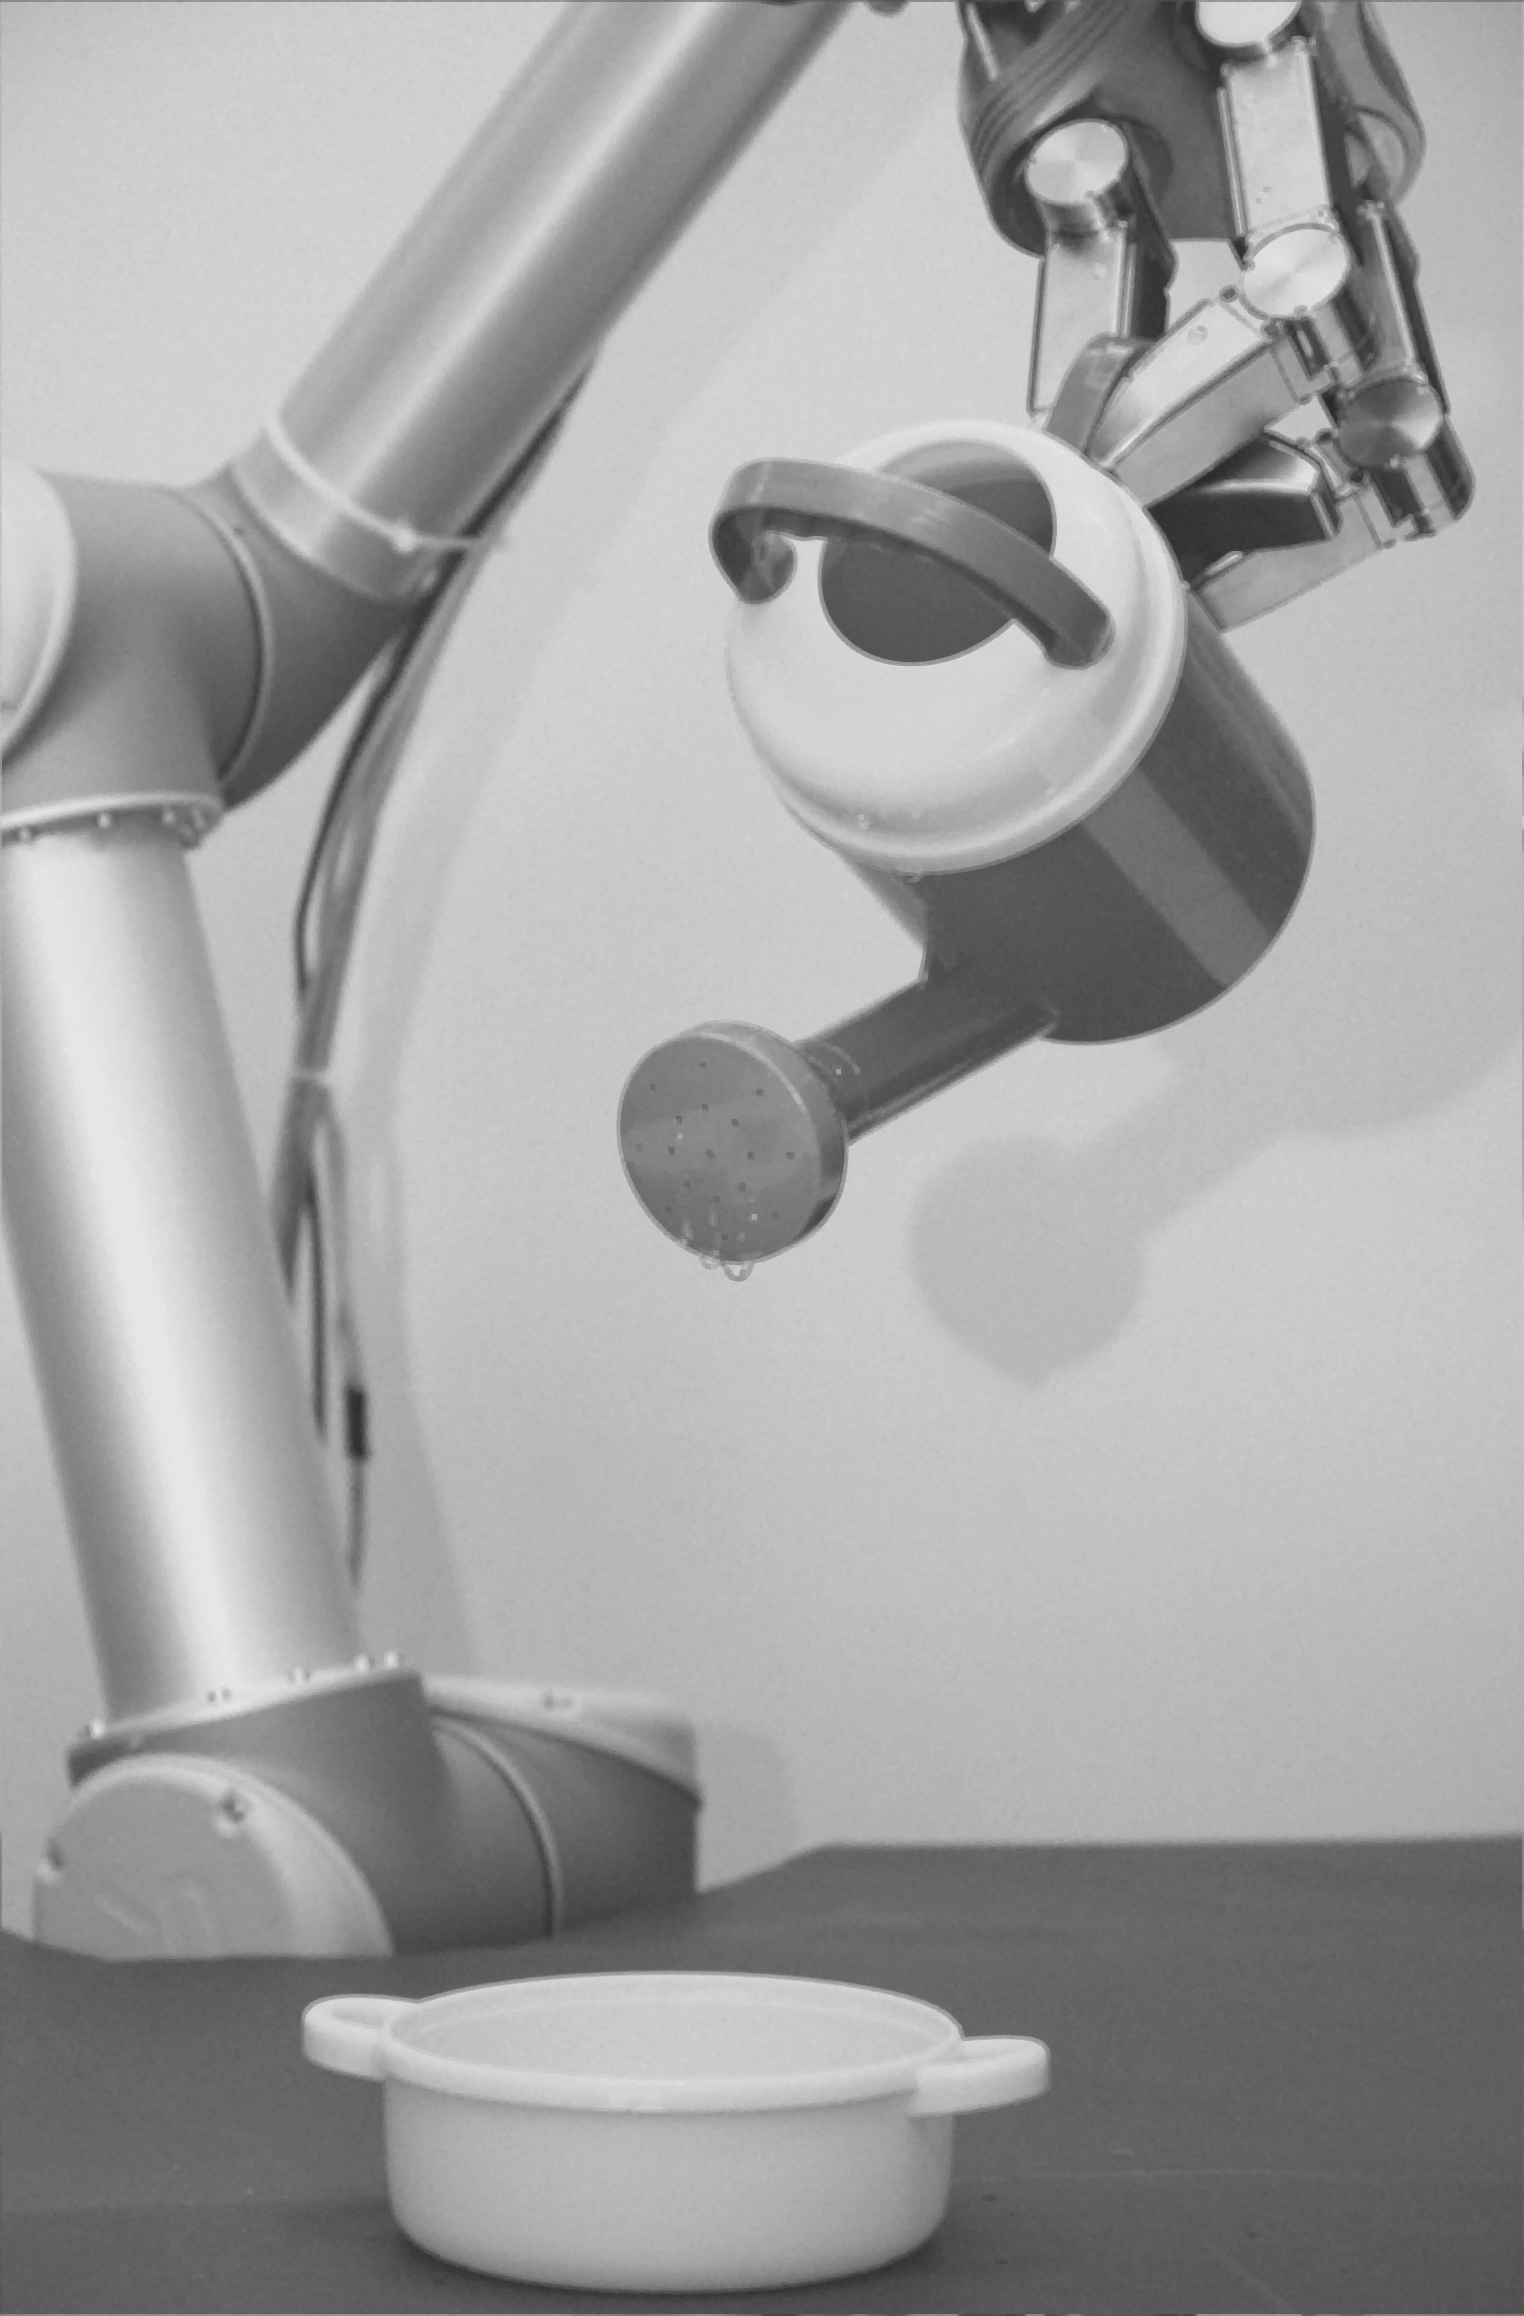
\includegraphics[width=\textwidth]{img3/test/contrast_5_0_9_final_img3.png}
    \end{subfigure}
    \begin{subfigure}[b]{0.1\textwidth}
        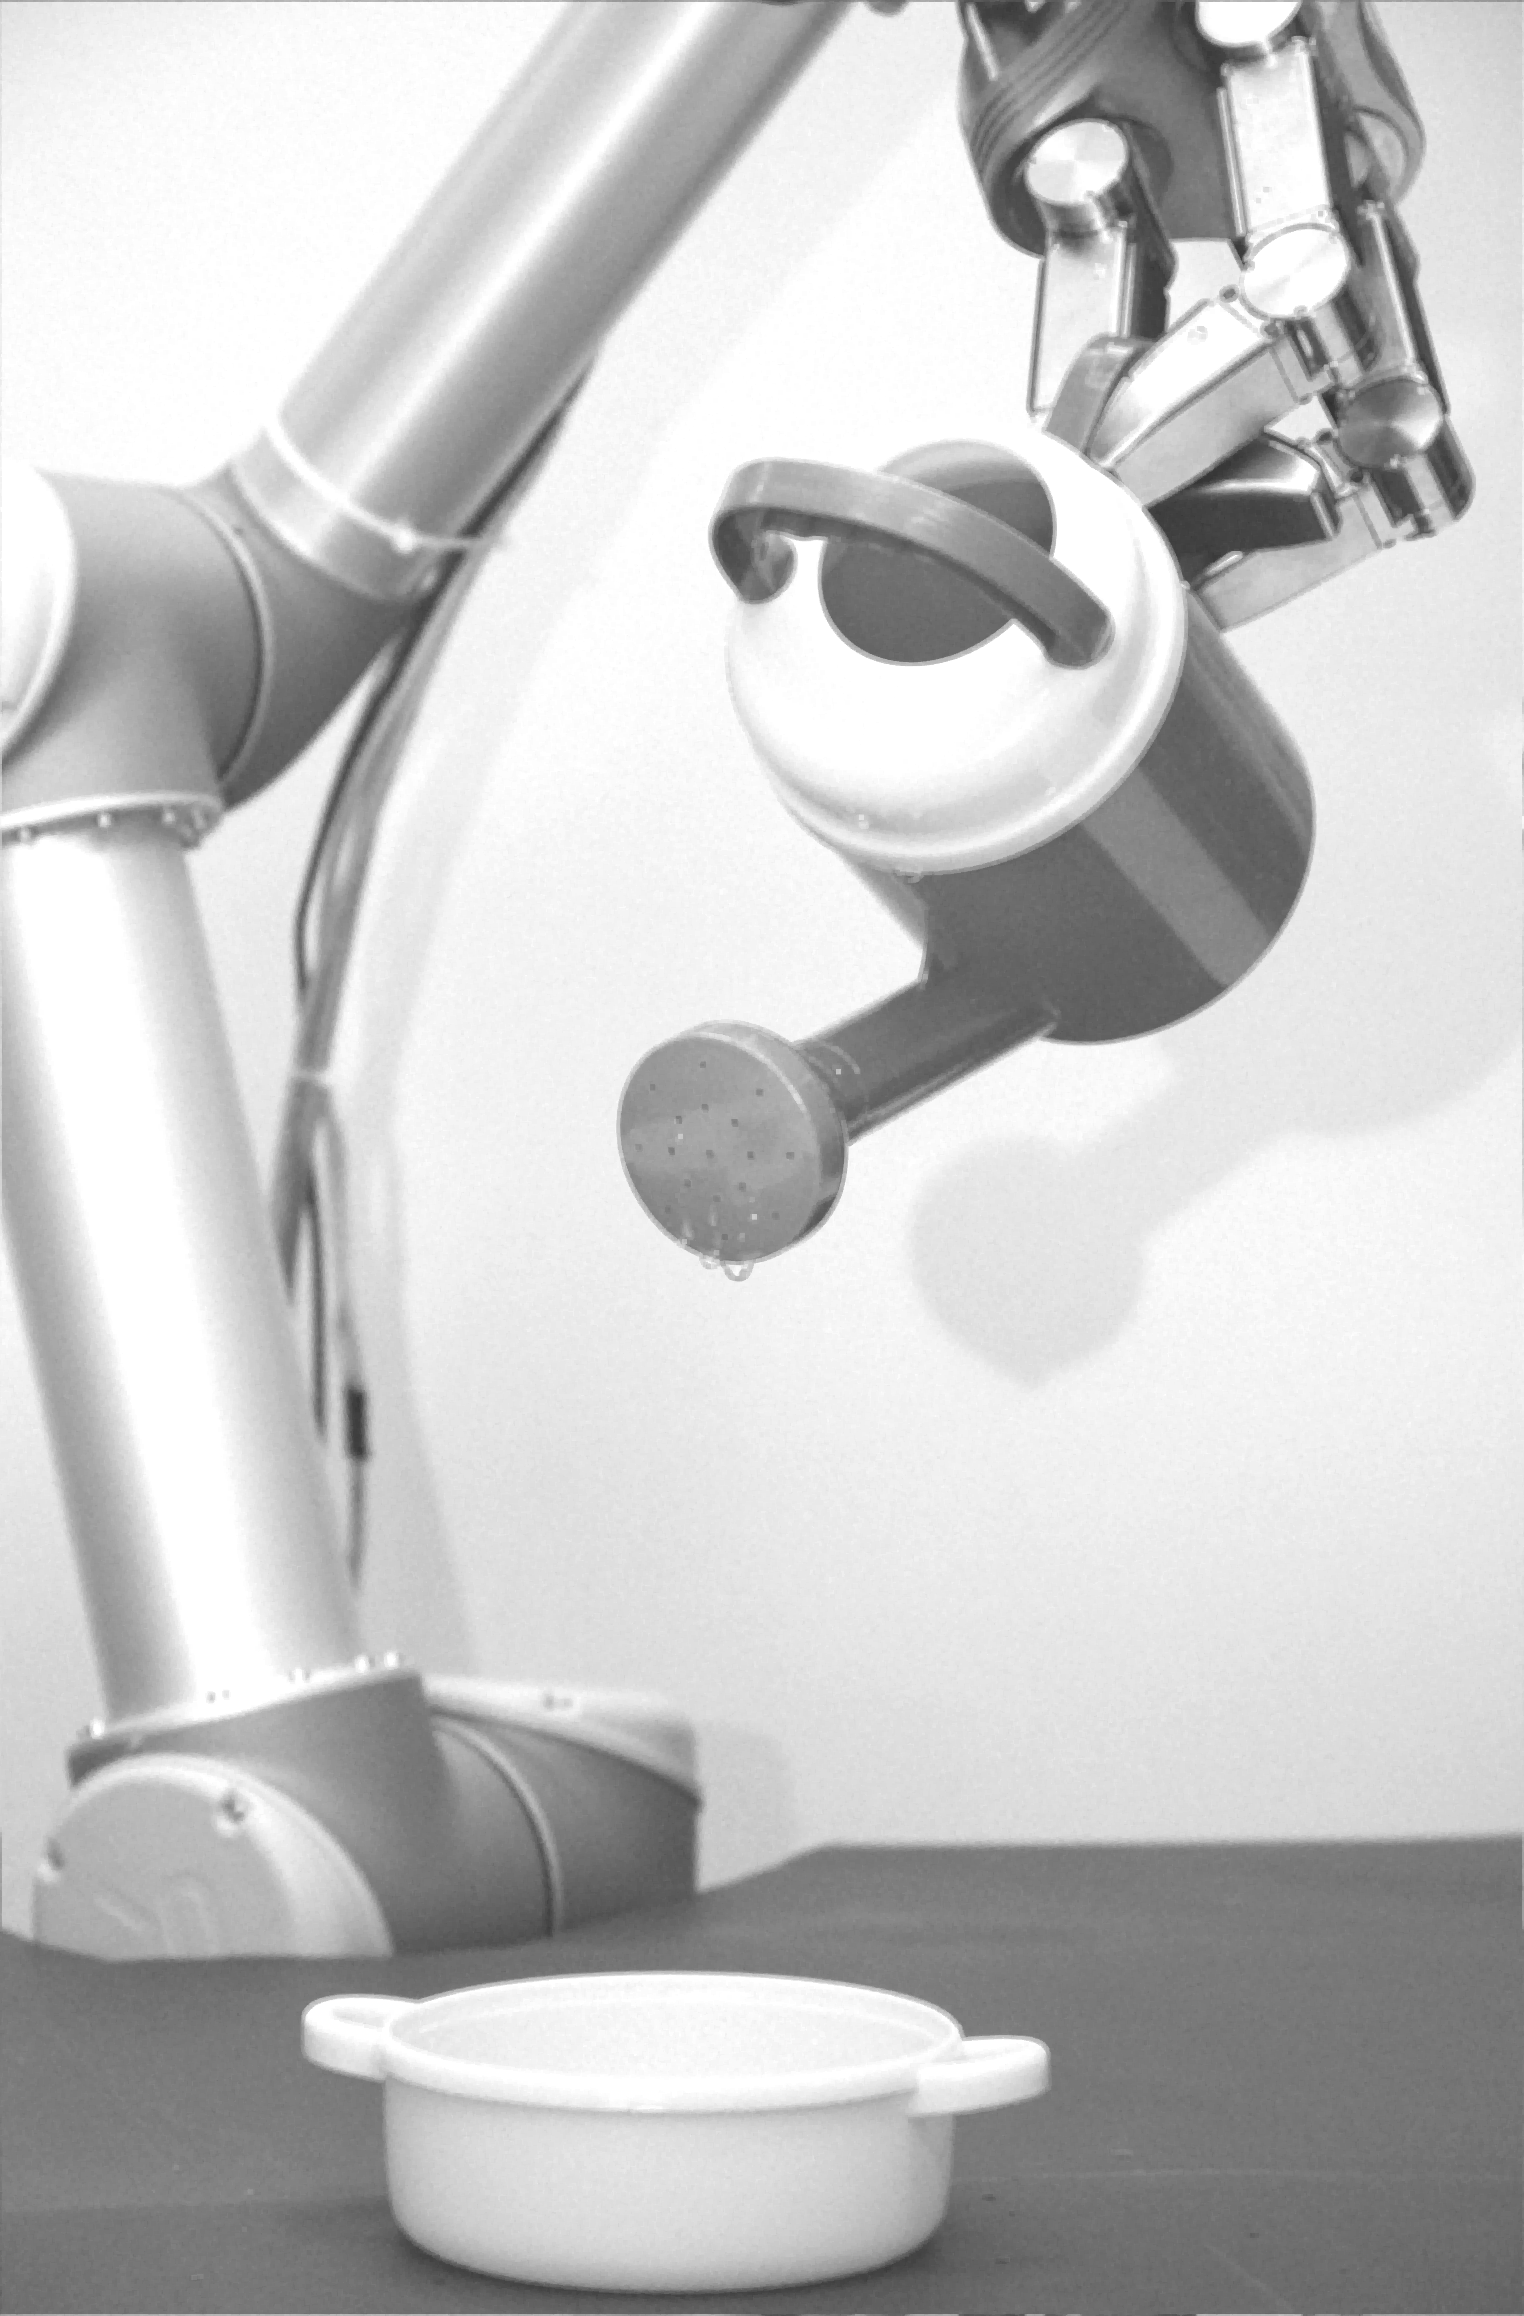
\includegraphics[width=\textwidth]{img3/test/contrast_5_1_1_final_img3.png}
    \end{subfigure}
        \begin{subfigure}[b]{0.1\textwidth}
        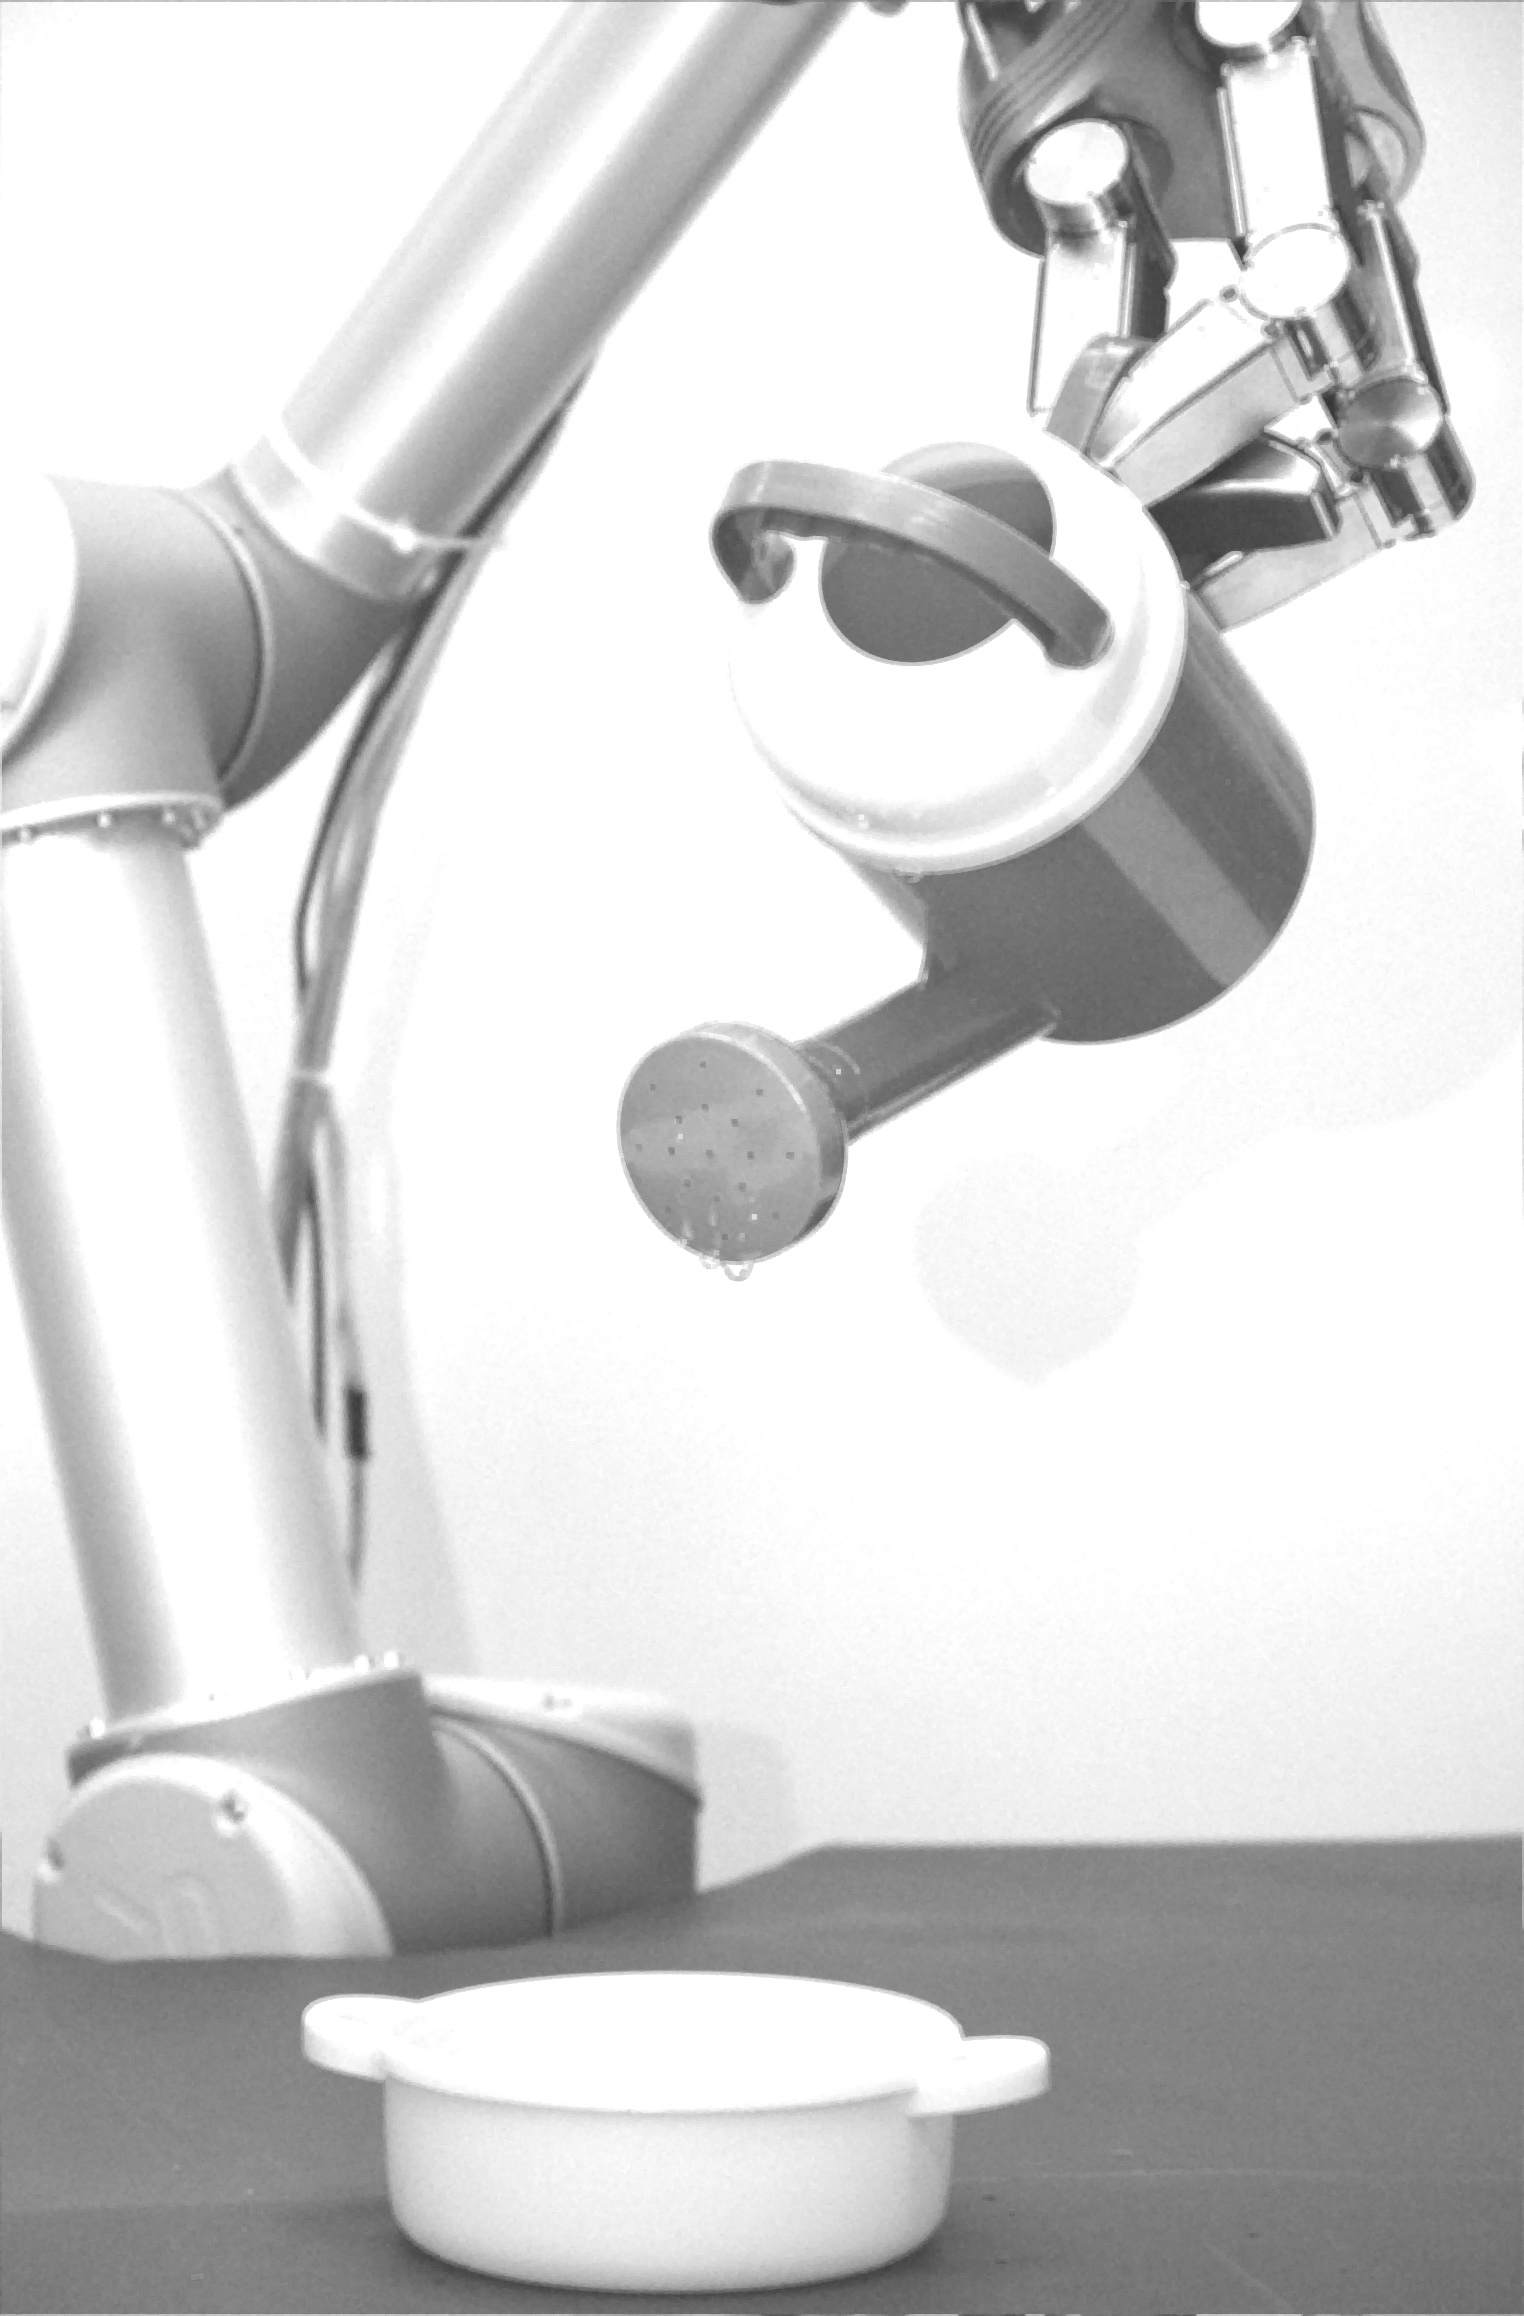
\includegraphics[width=\textwidth]{img3/test/contrast_5_1_2_final_img3.png}
    \end{subfigure}
        \begin{subfigure}[b]{0.1\textwidth}
        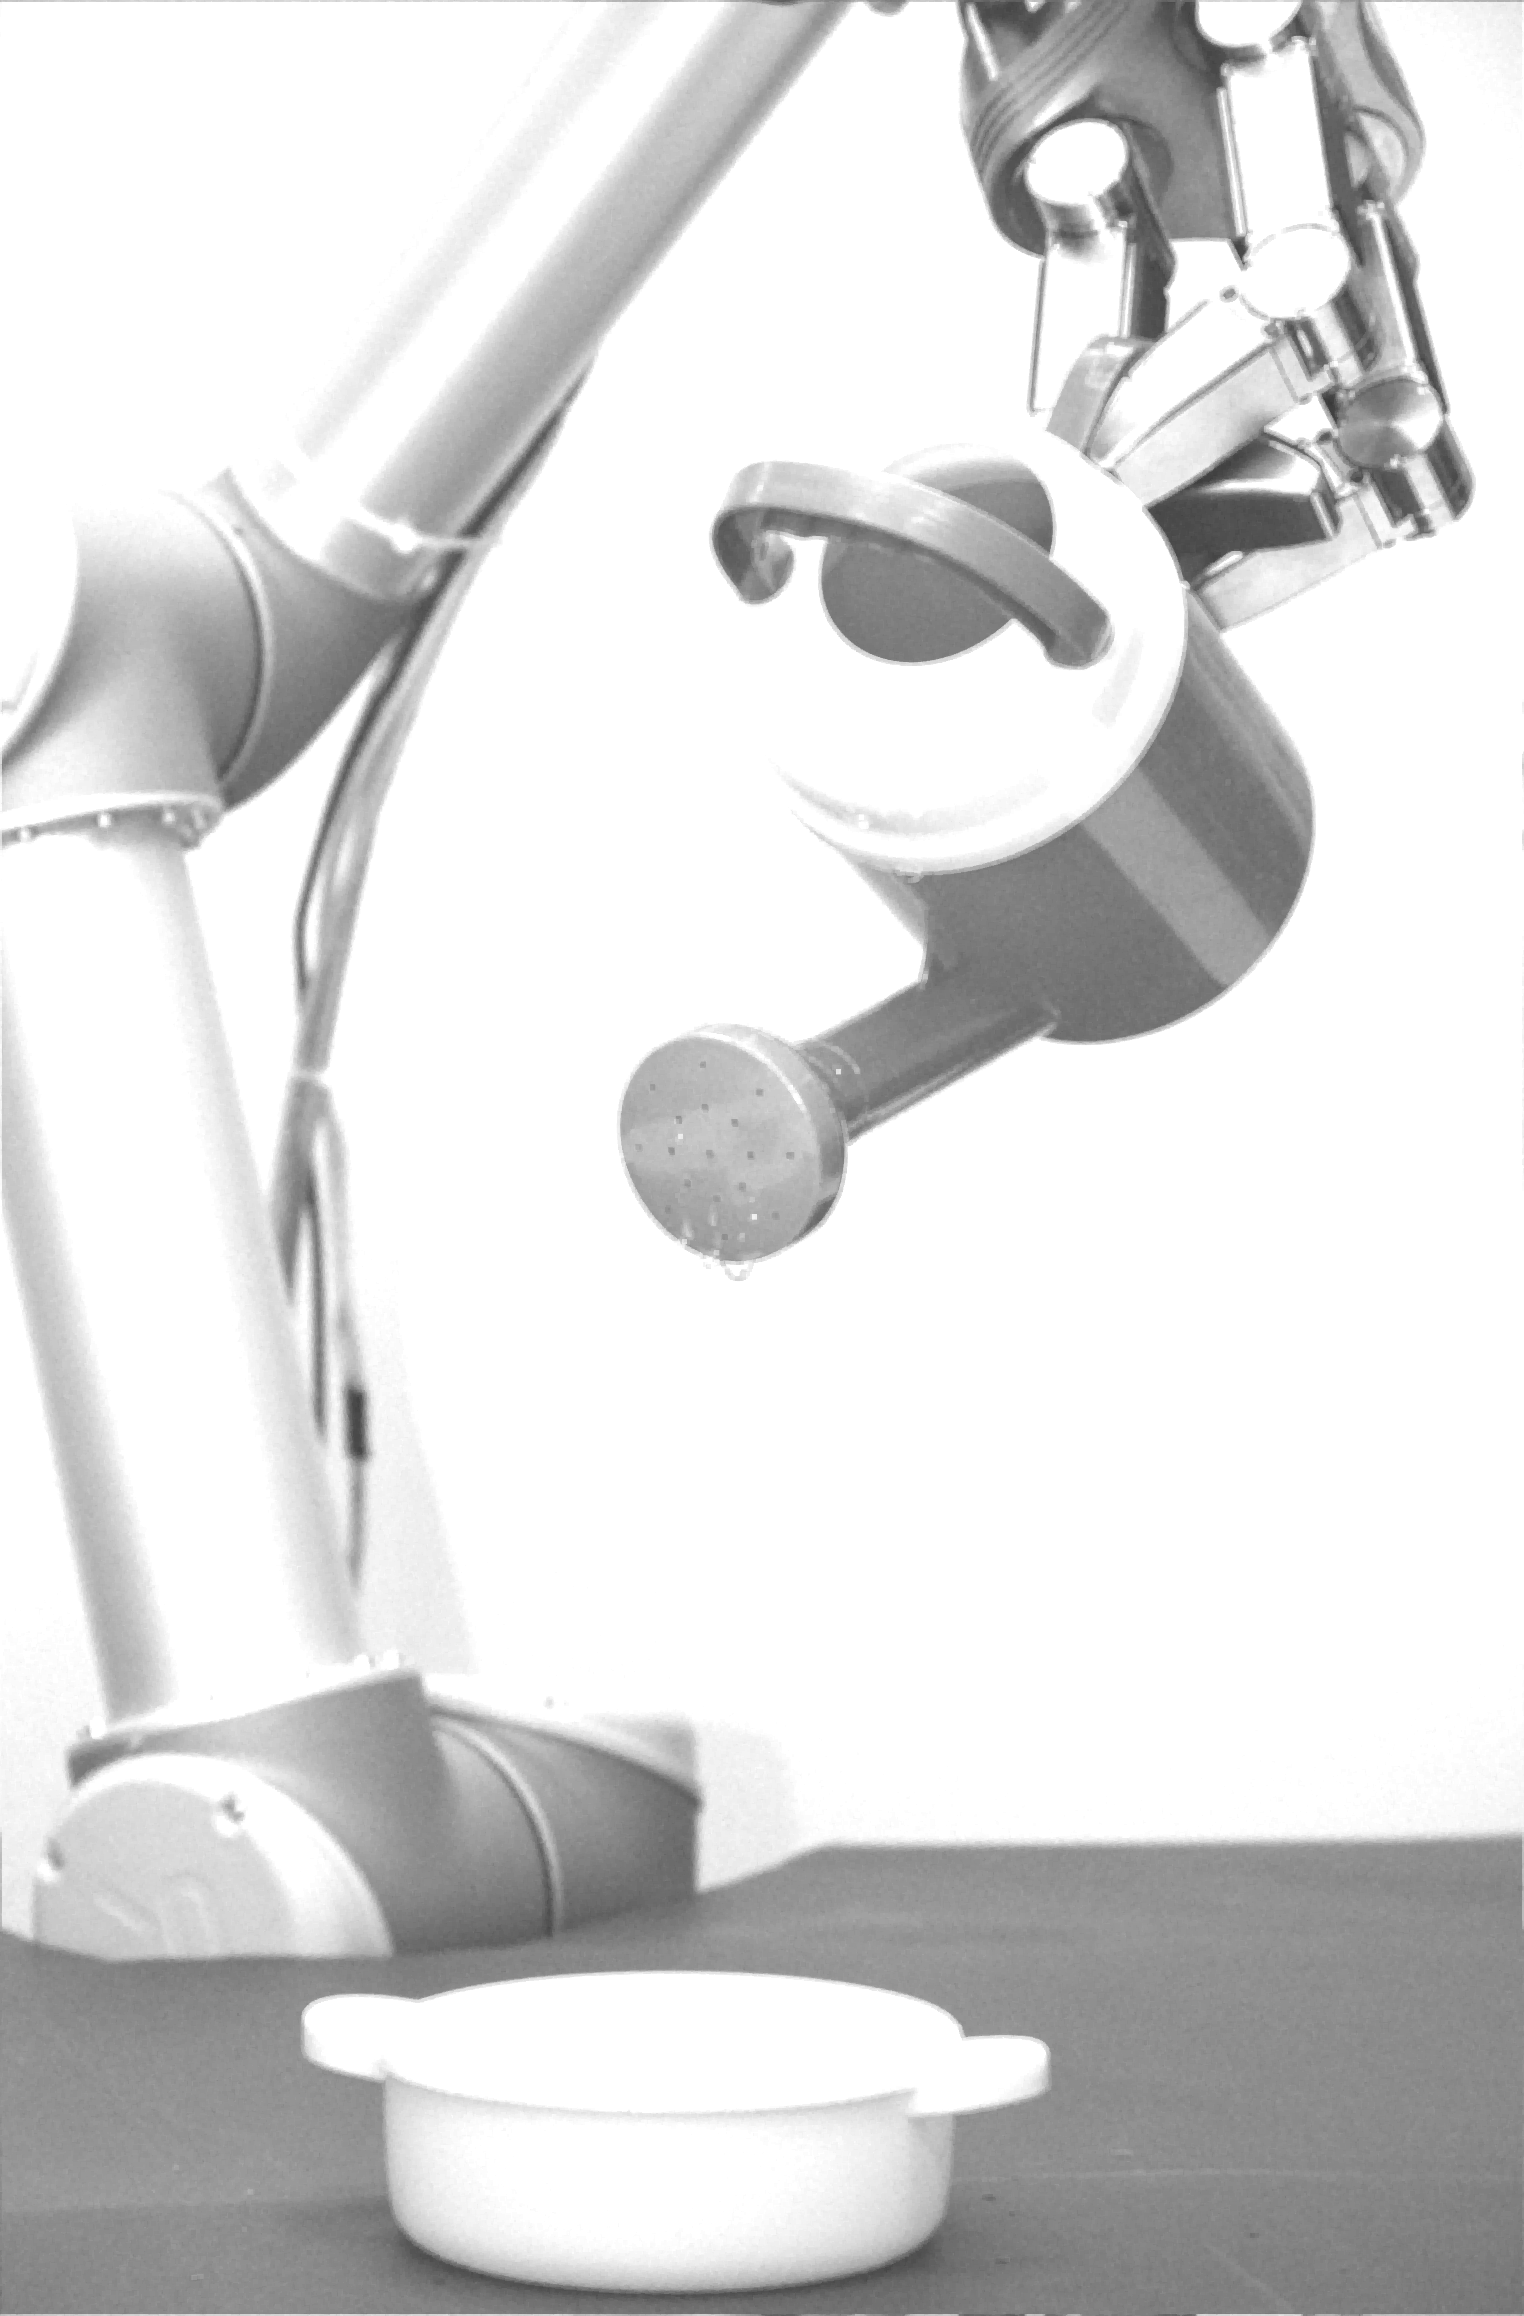
\includegraphics[width=\textwidth]{img3/test/contrast_5_1_3_final_img3.png}
    \end{subfigure}
        \begin{subfigure}[b]{0.1\textwidth}
        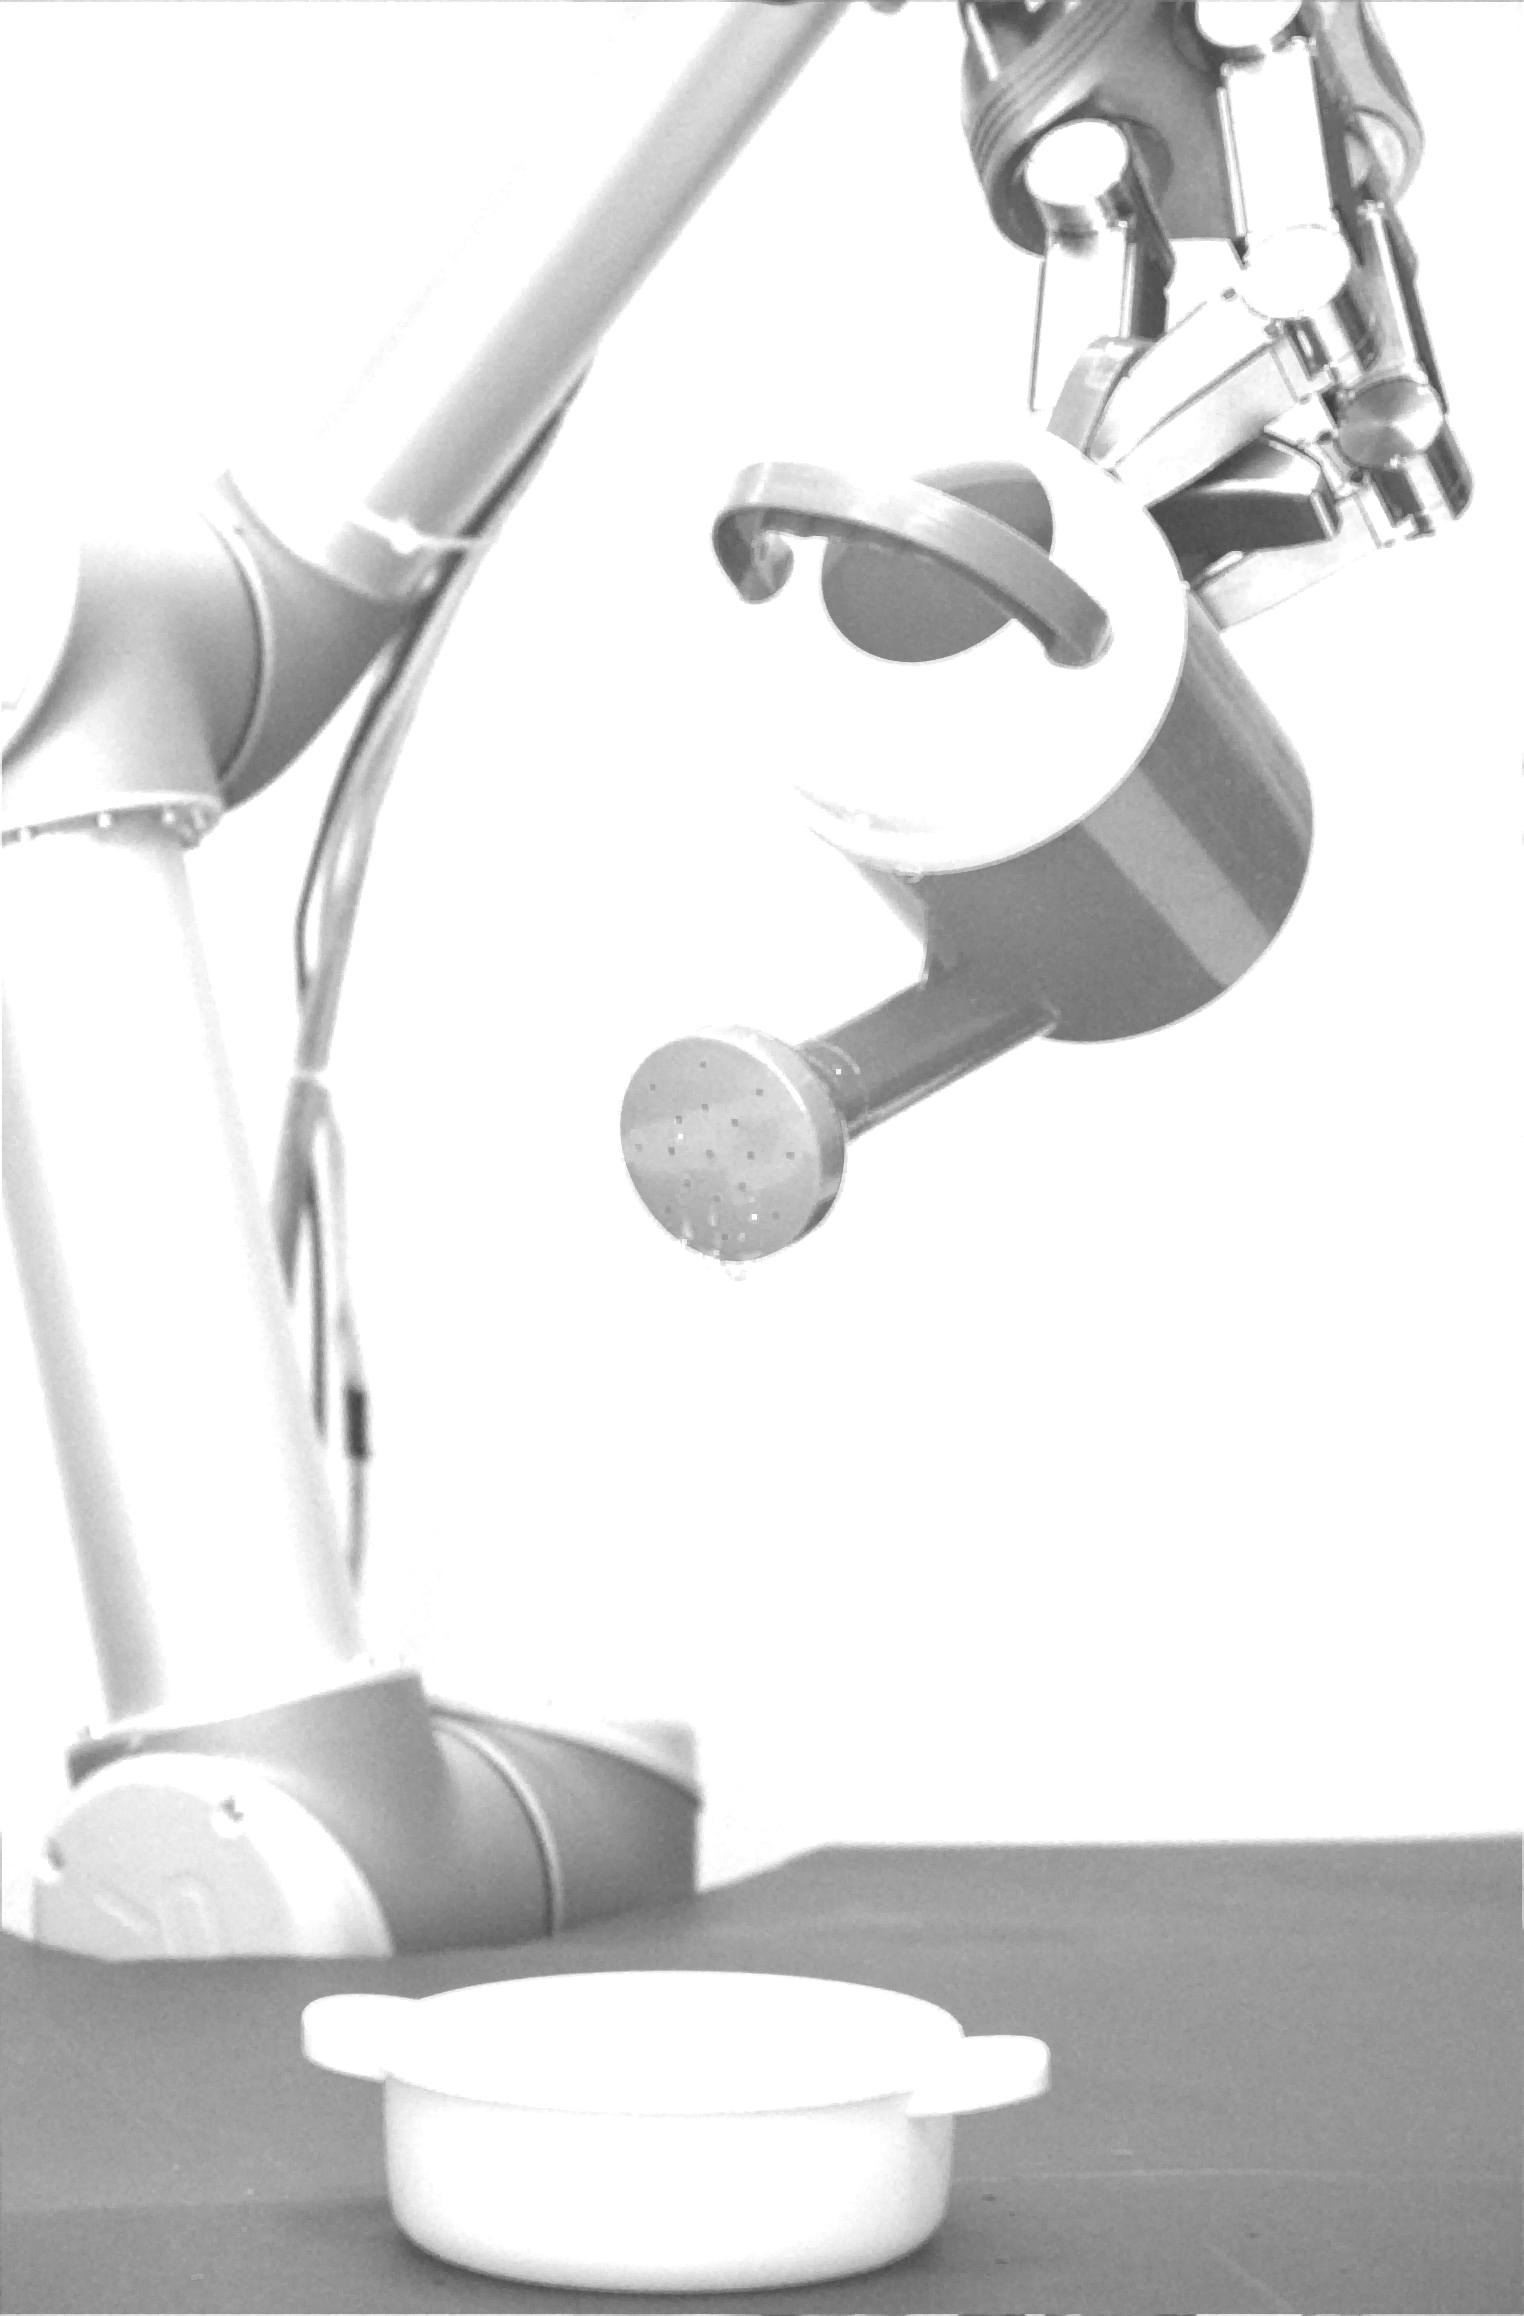
\includegraphics[width=\textwidth]{img3/test/contrast_5_1_4_final_img3.png}
    \end{subfigure}
        \begin{subfigure}[b]{0.1\textwidth}
        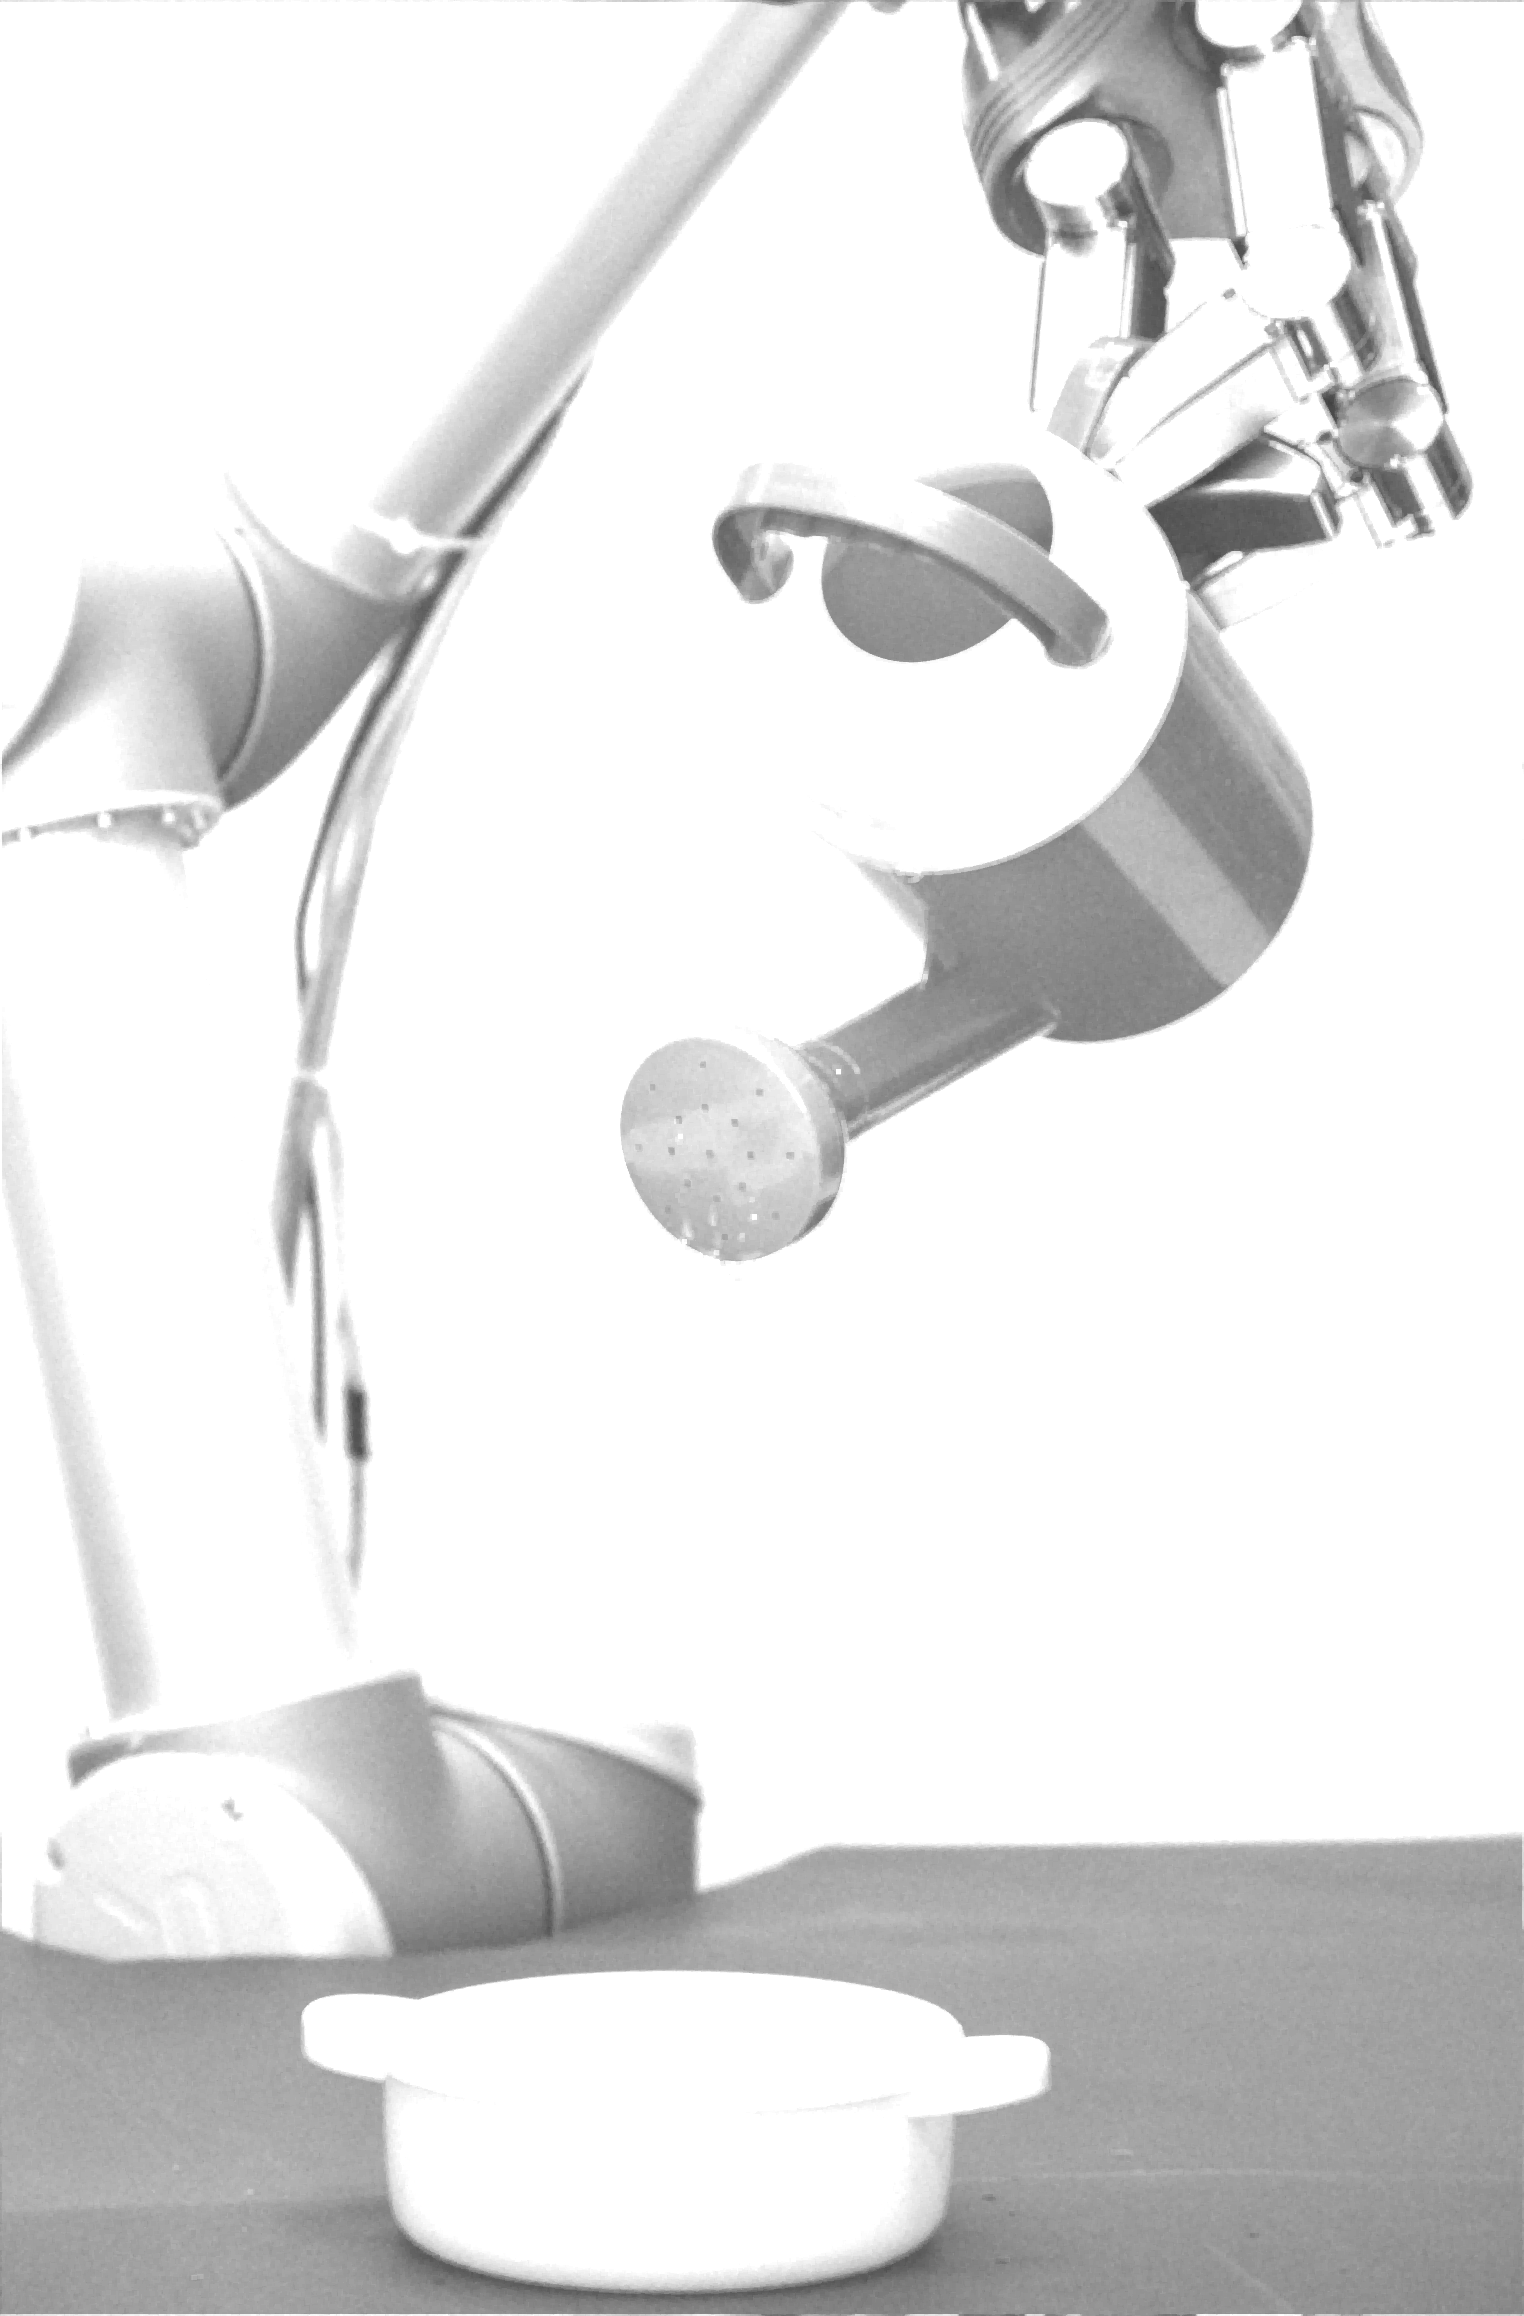
\includegraphics[width=\textwidth]{img3/test/contrast_5_1_5_final_img3.png}
    \end{subfigure}
        \begin{subfigure}[b]{0.1\textwidth}
        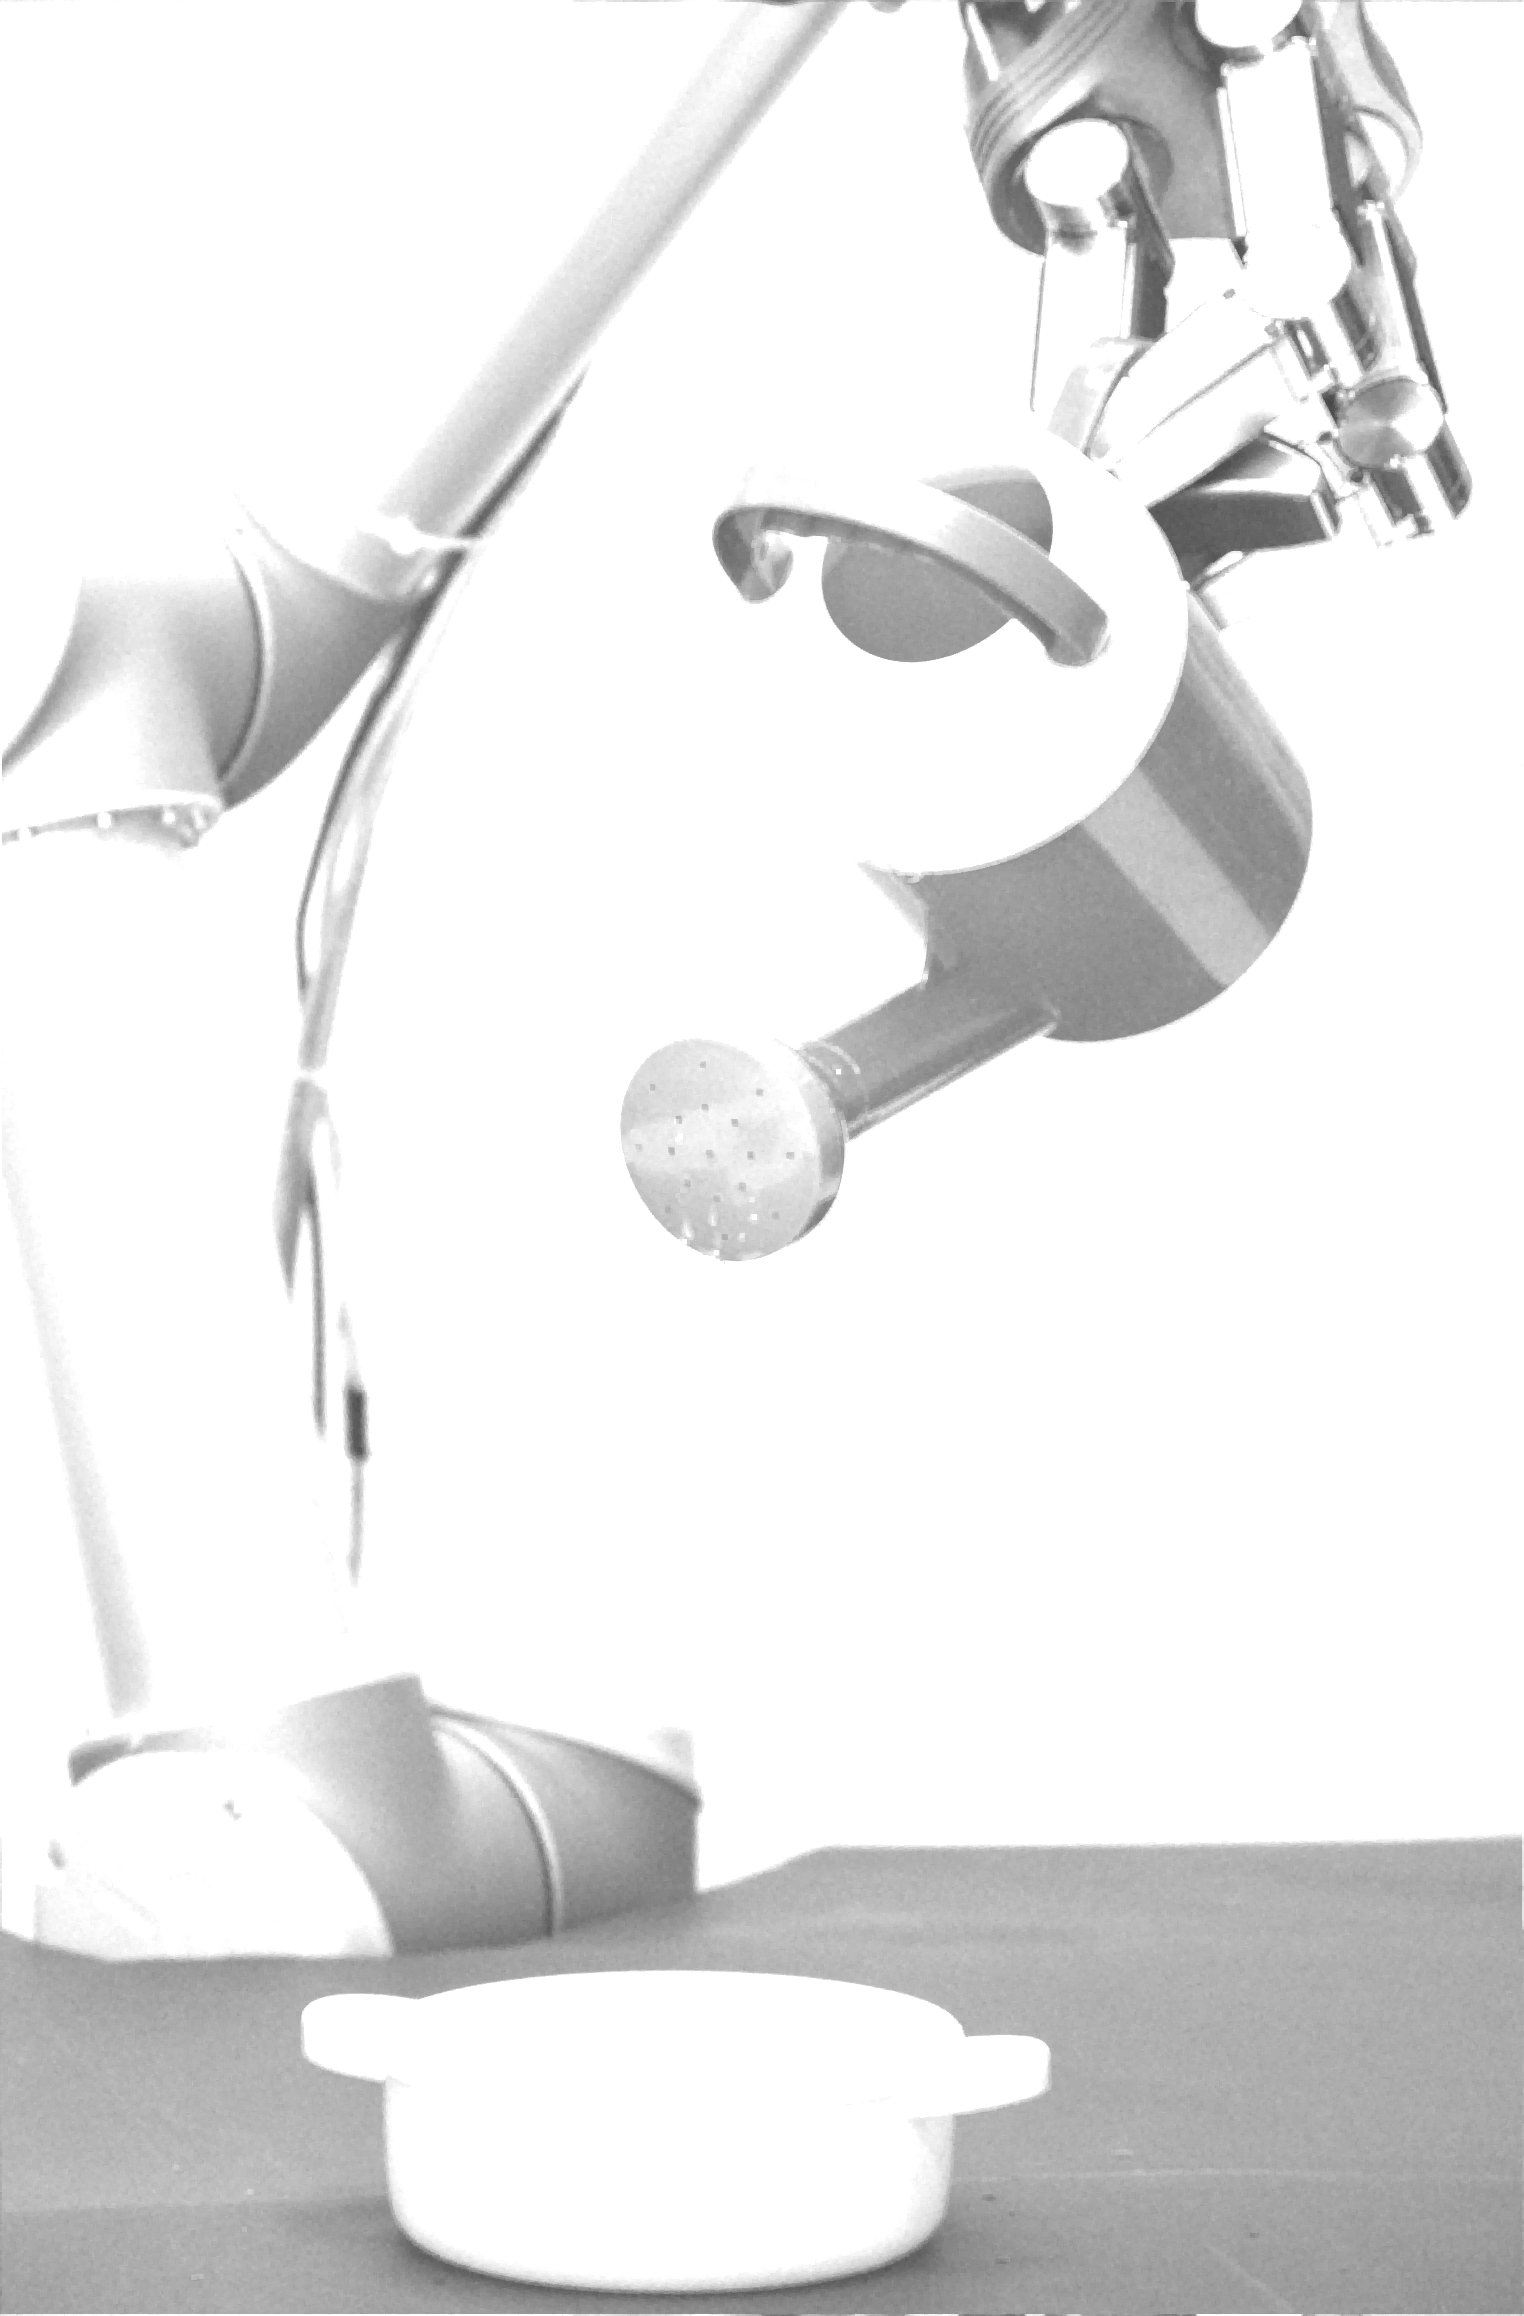
\includegraphics[width=\textwidth]{img3/test/contrast_5_1_6_final_img3.png}
    \end{subfigure}
        \begin{subfigure}[b]{0.1\textwidth}
        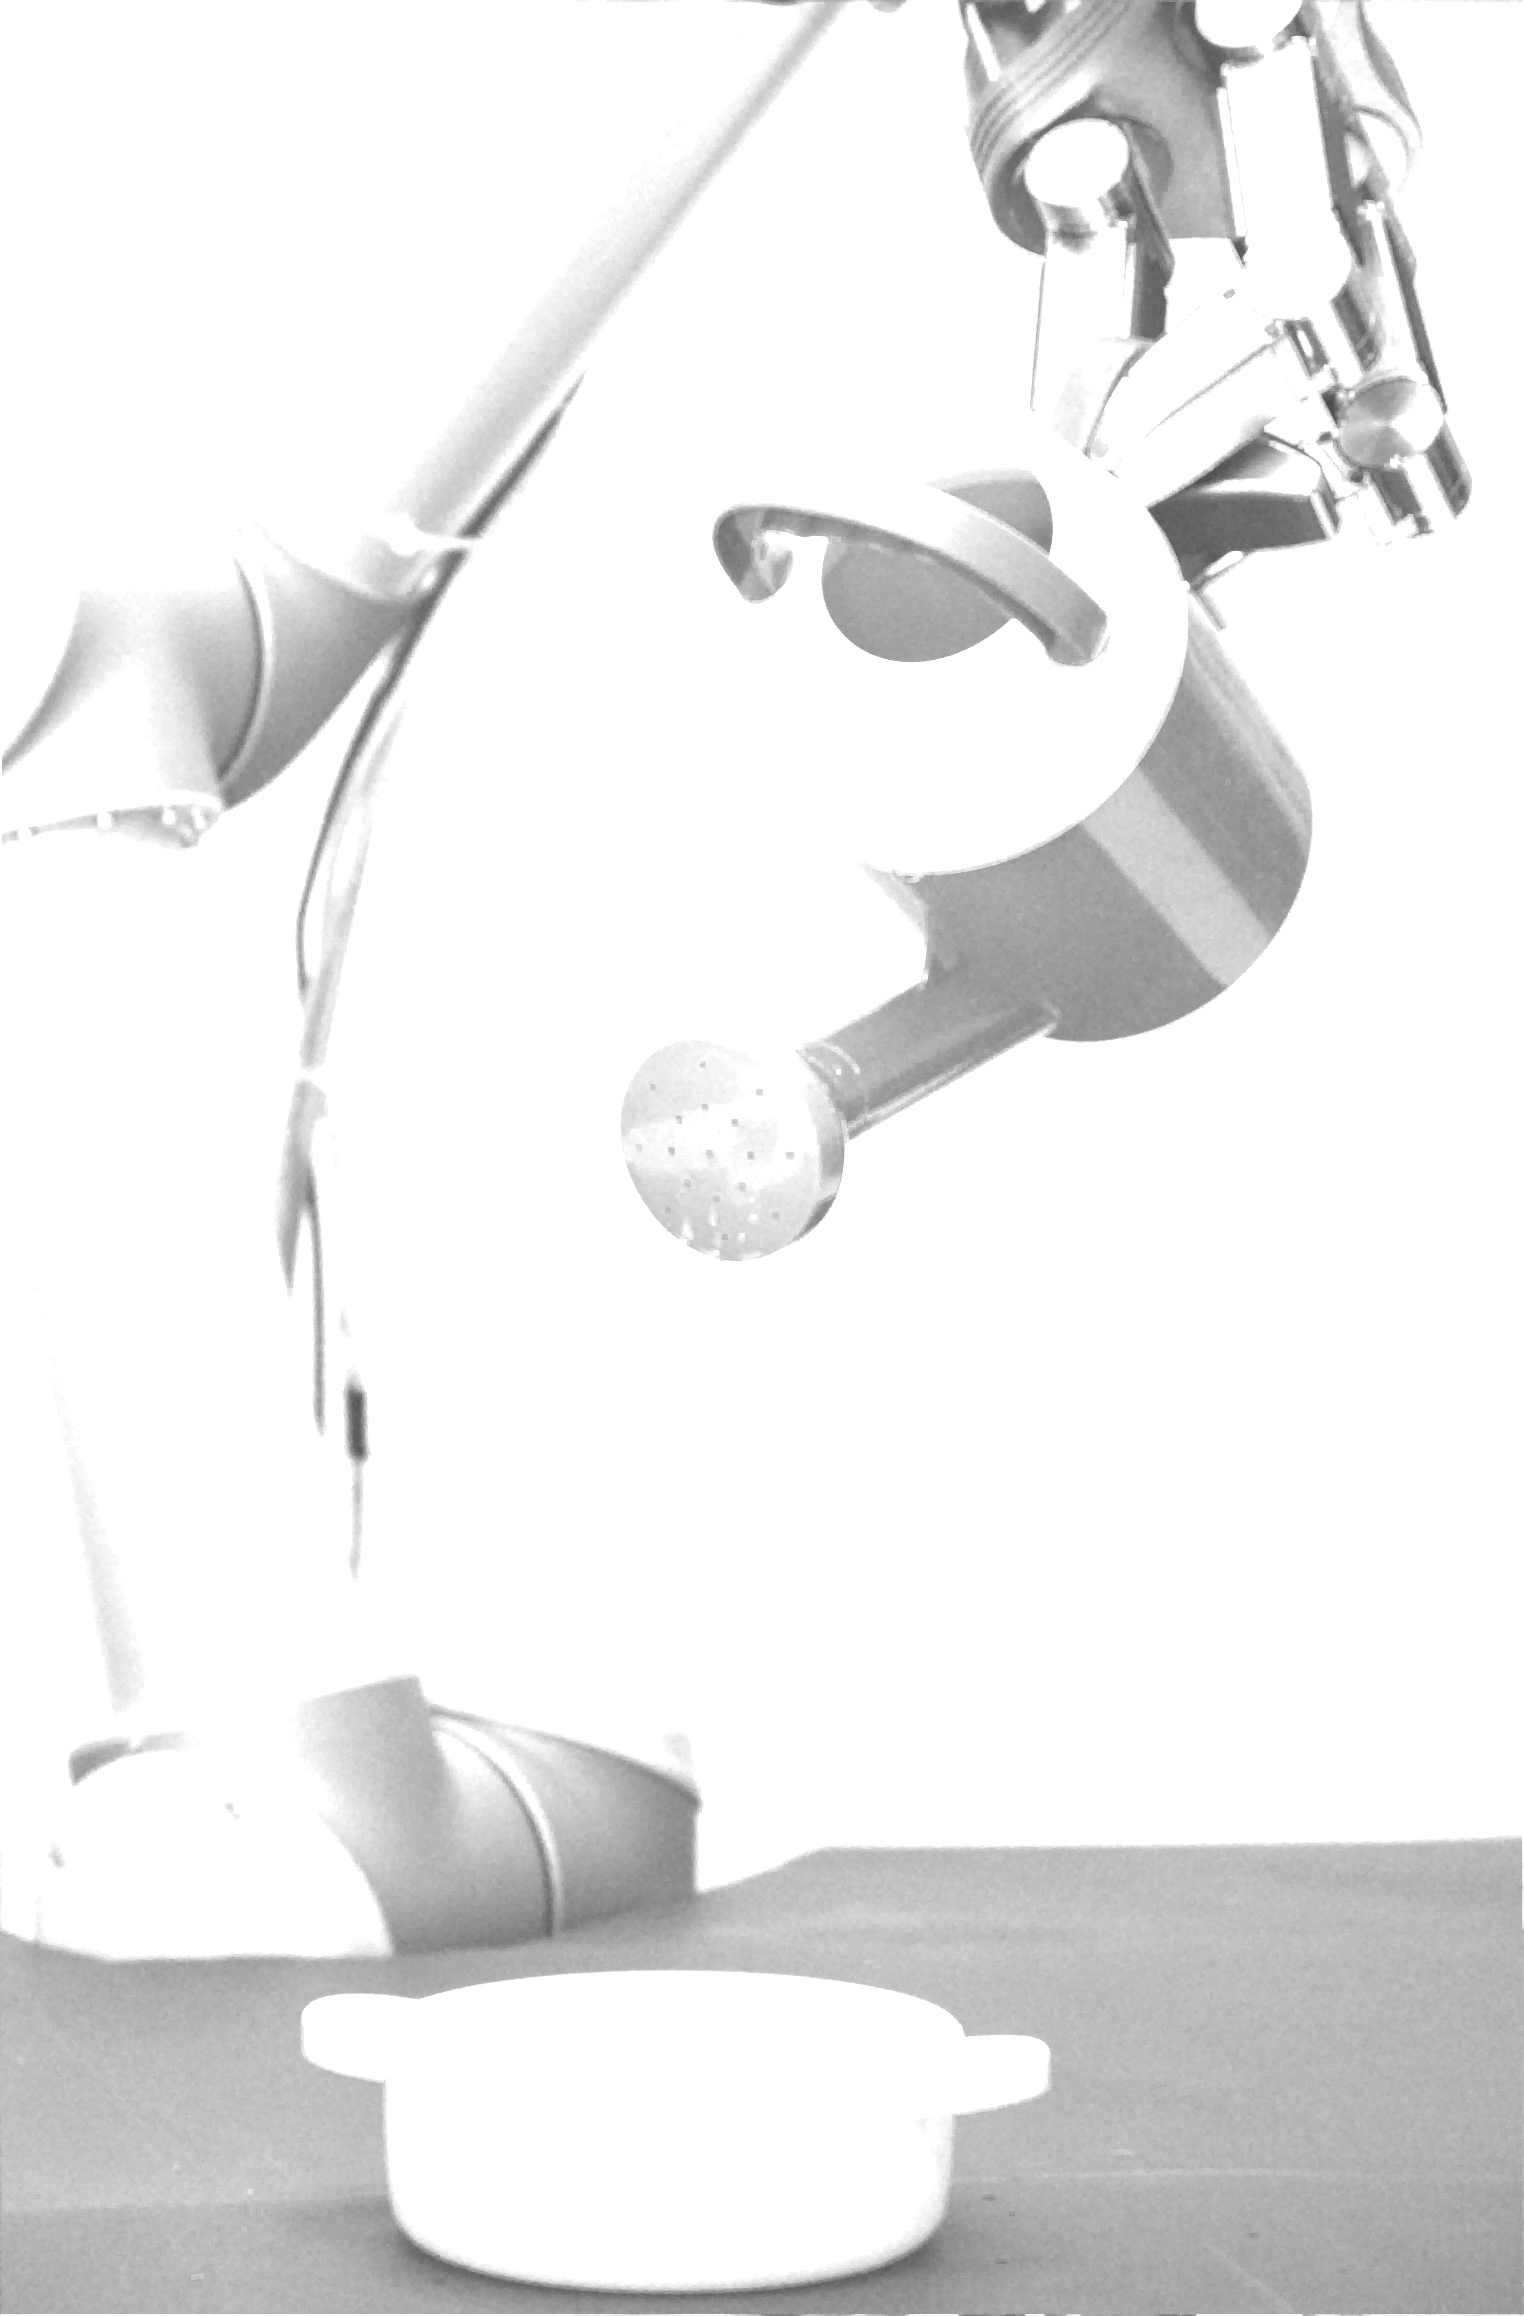
\includegraphics[width=\textwidth]{img3/test/contrast_5_1_7_final_img3.png}
    \end{subfigure}
        \begin{subfigure}[b]{0.1\textwidth}
        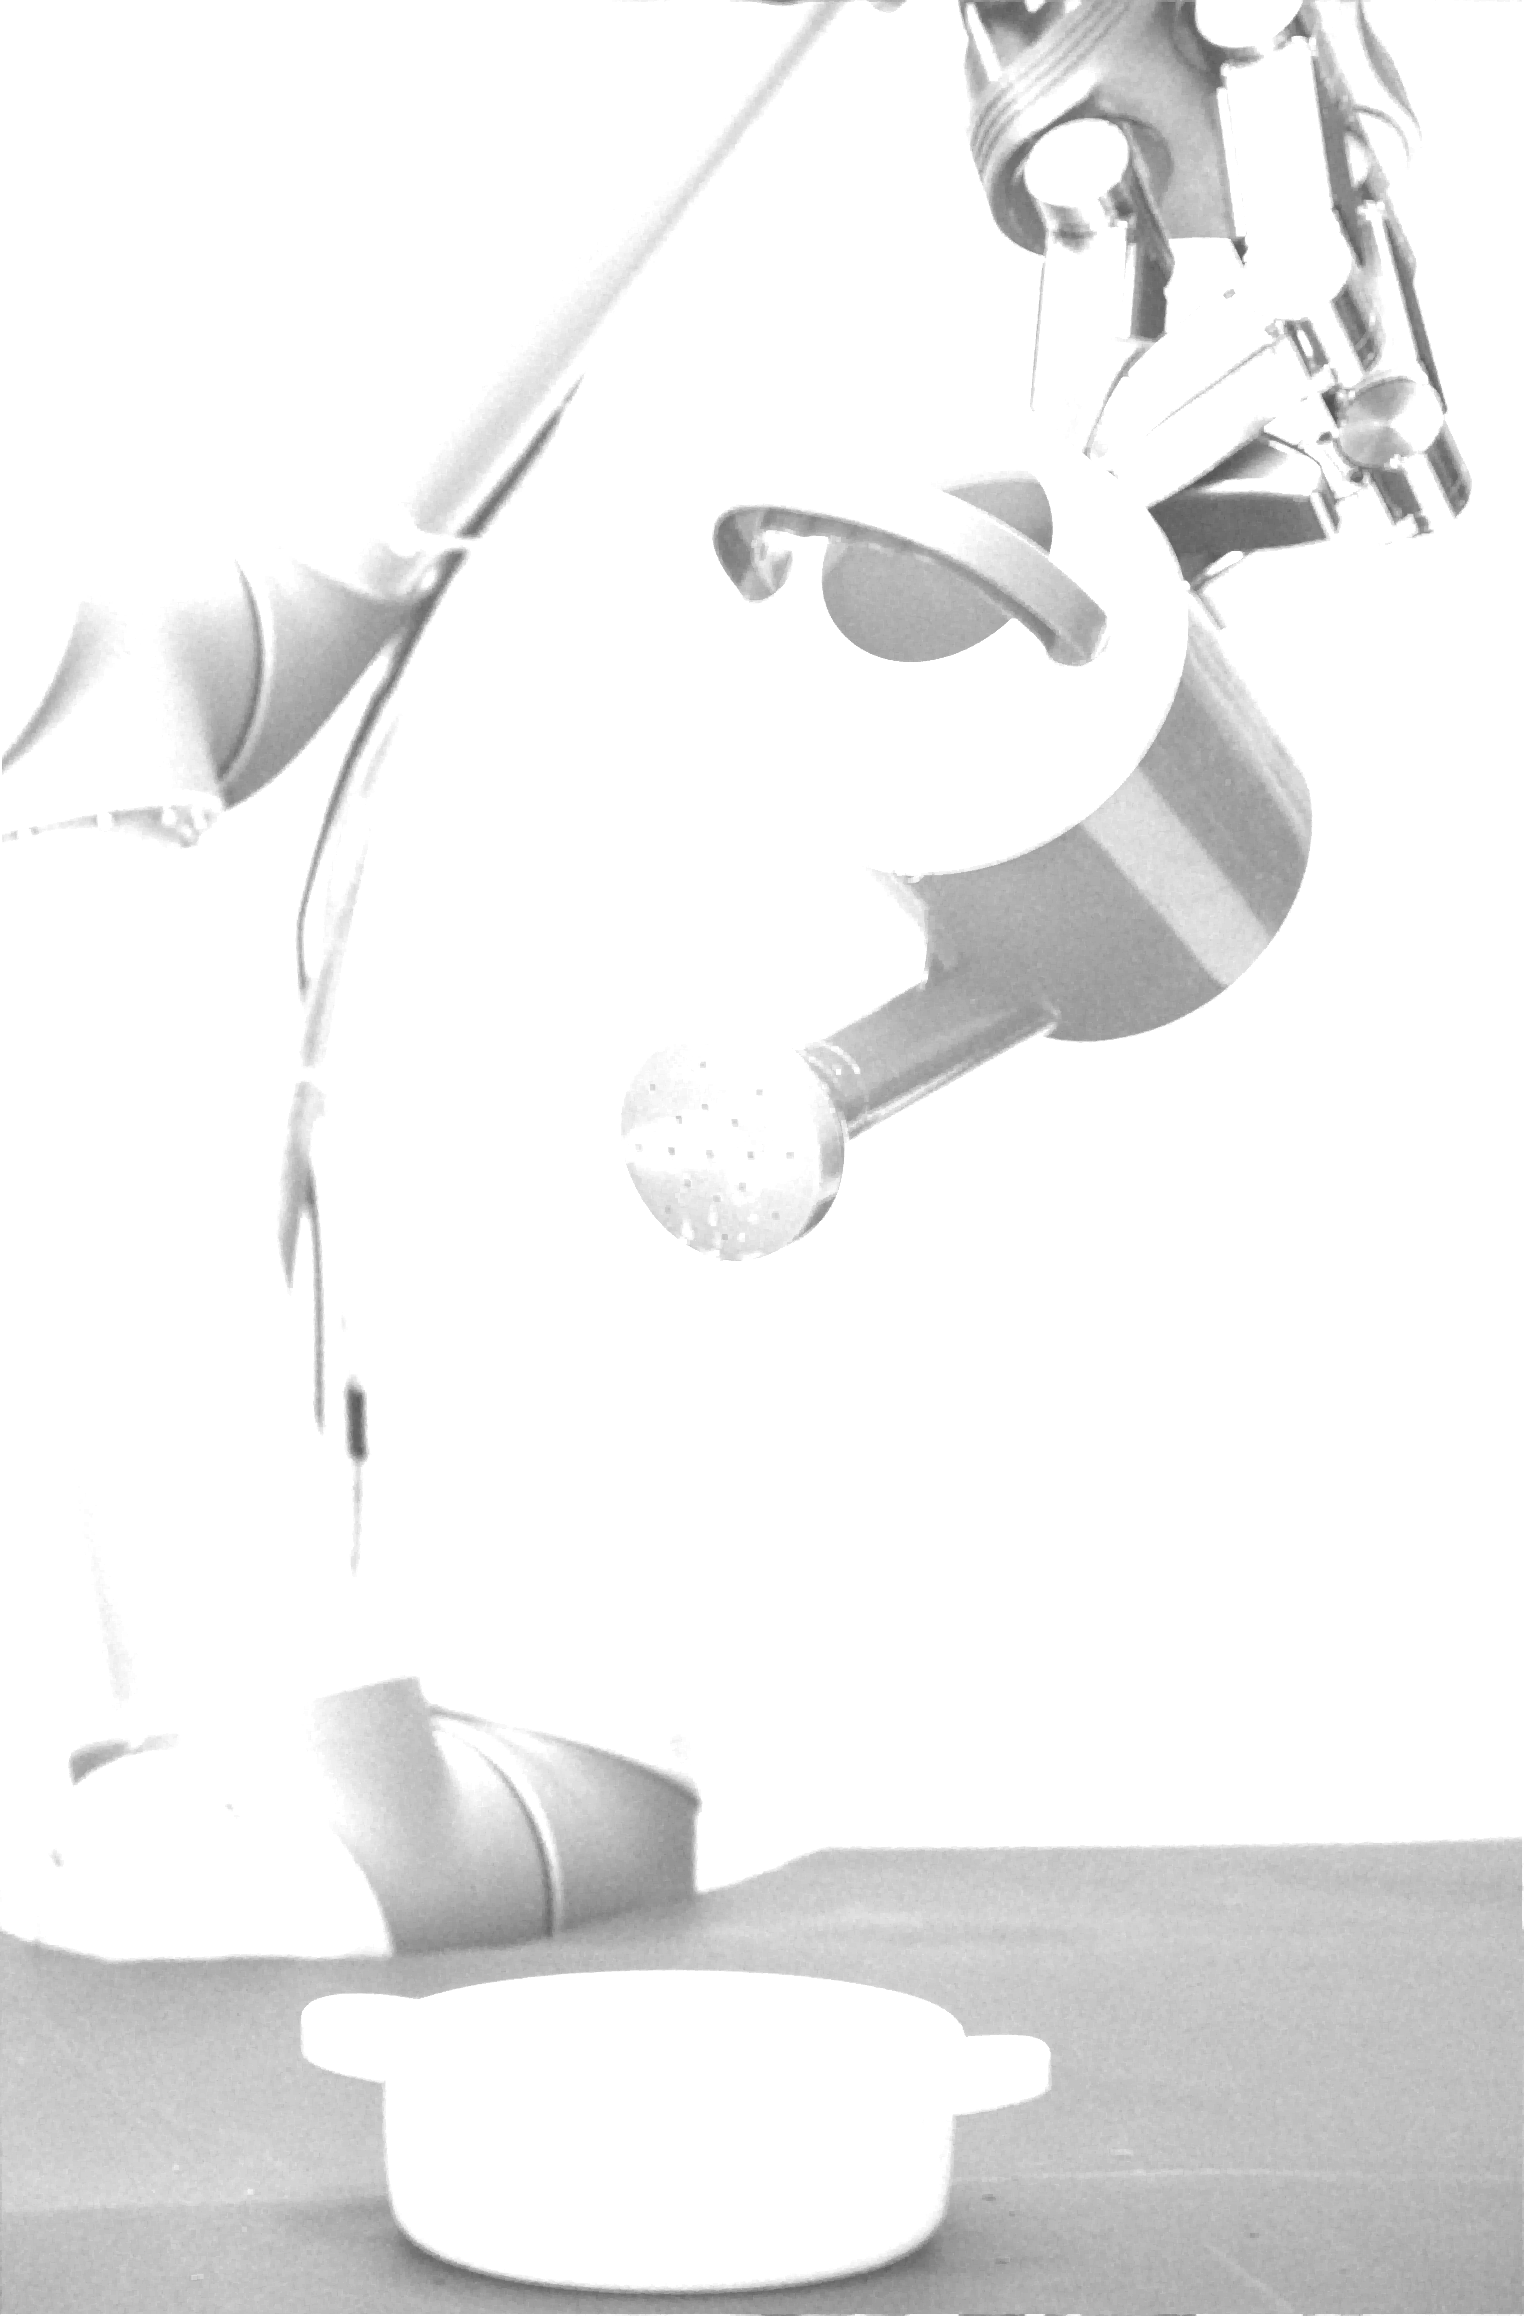
\includegraphics[width=\textwidth]{img3/test/contrast_5_1_8_final_img3.png}
    \end{subfigure}
        \begin{subfigure}[b]{0.1\textwidth}
        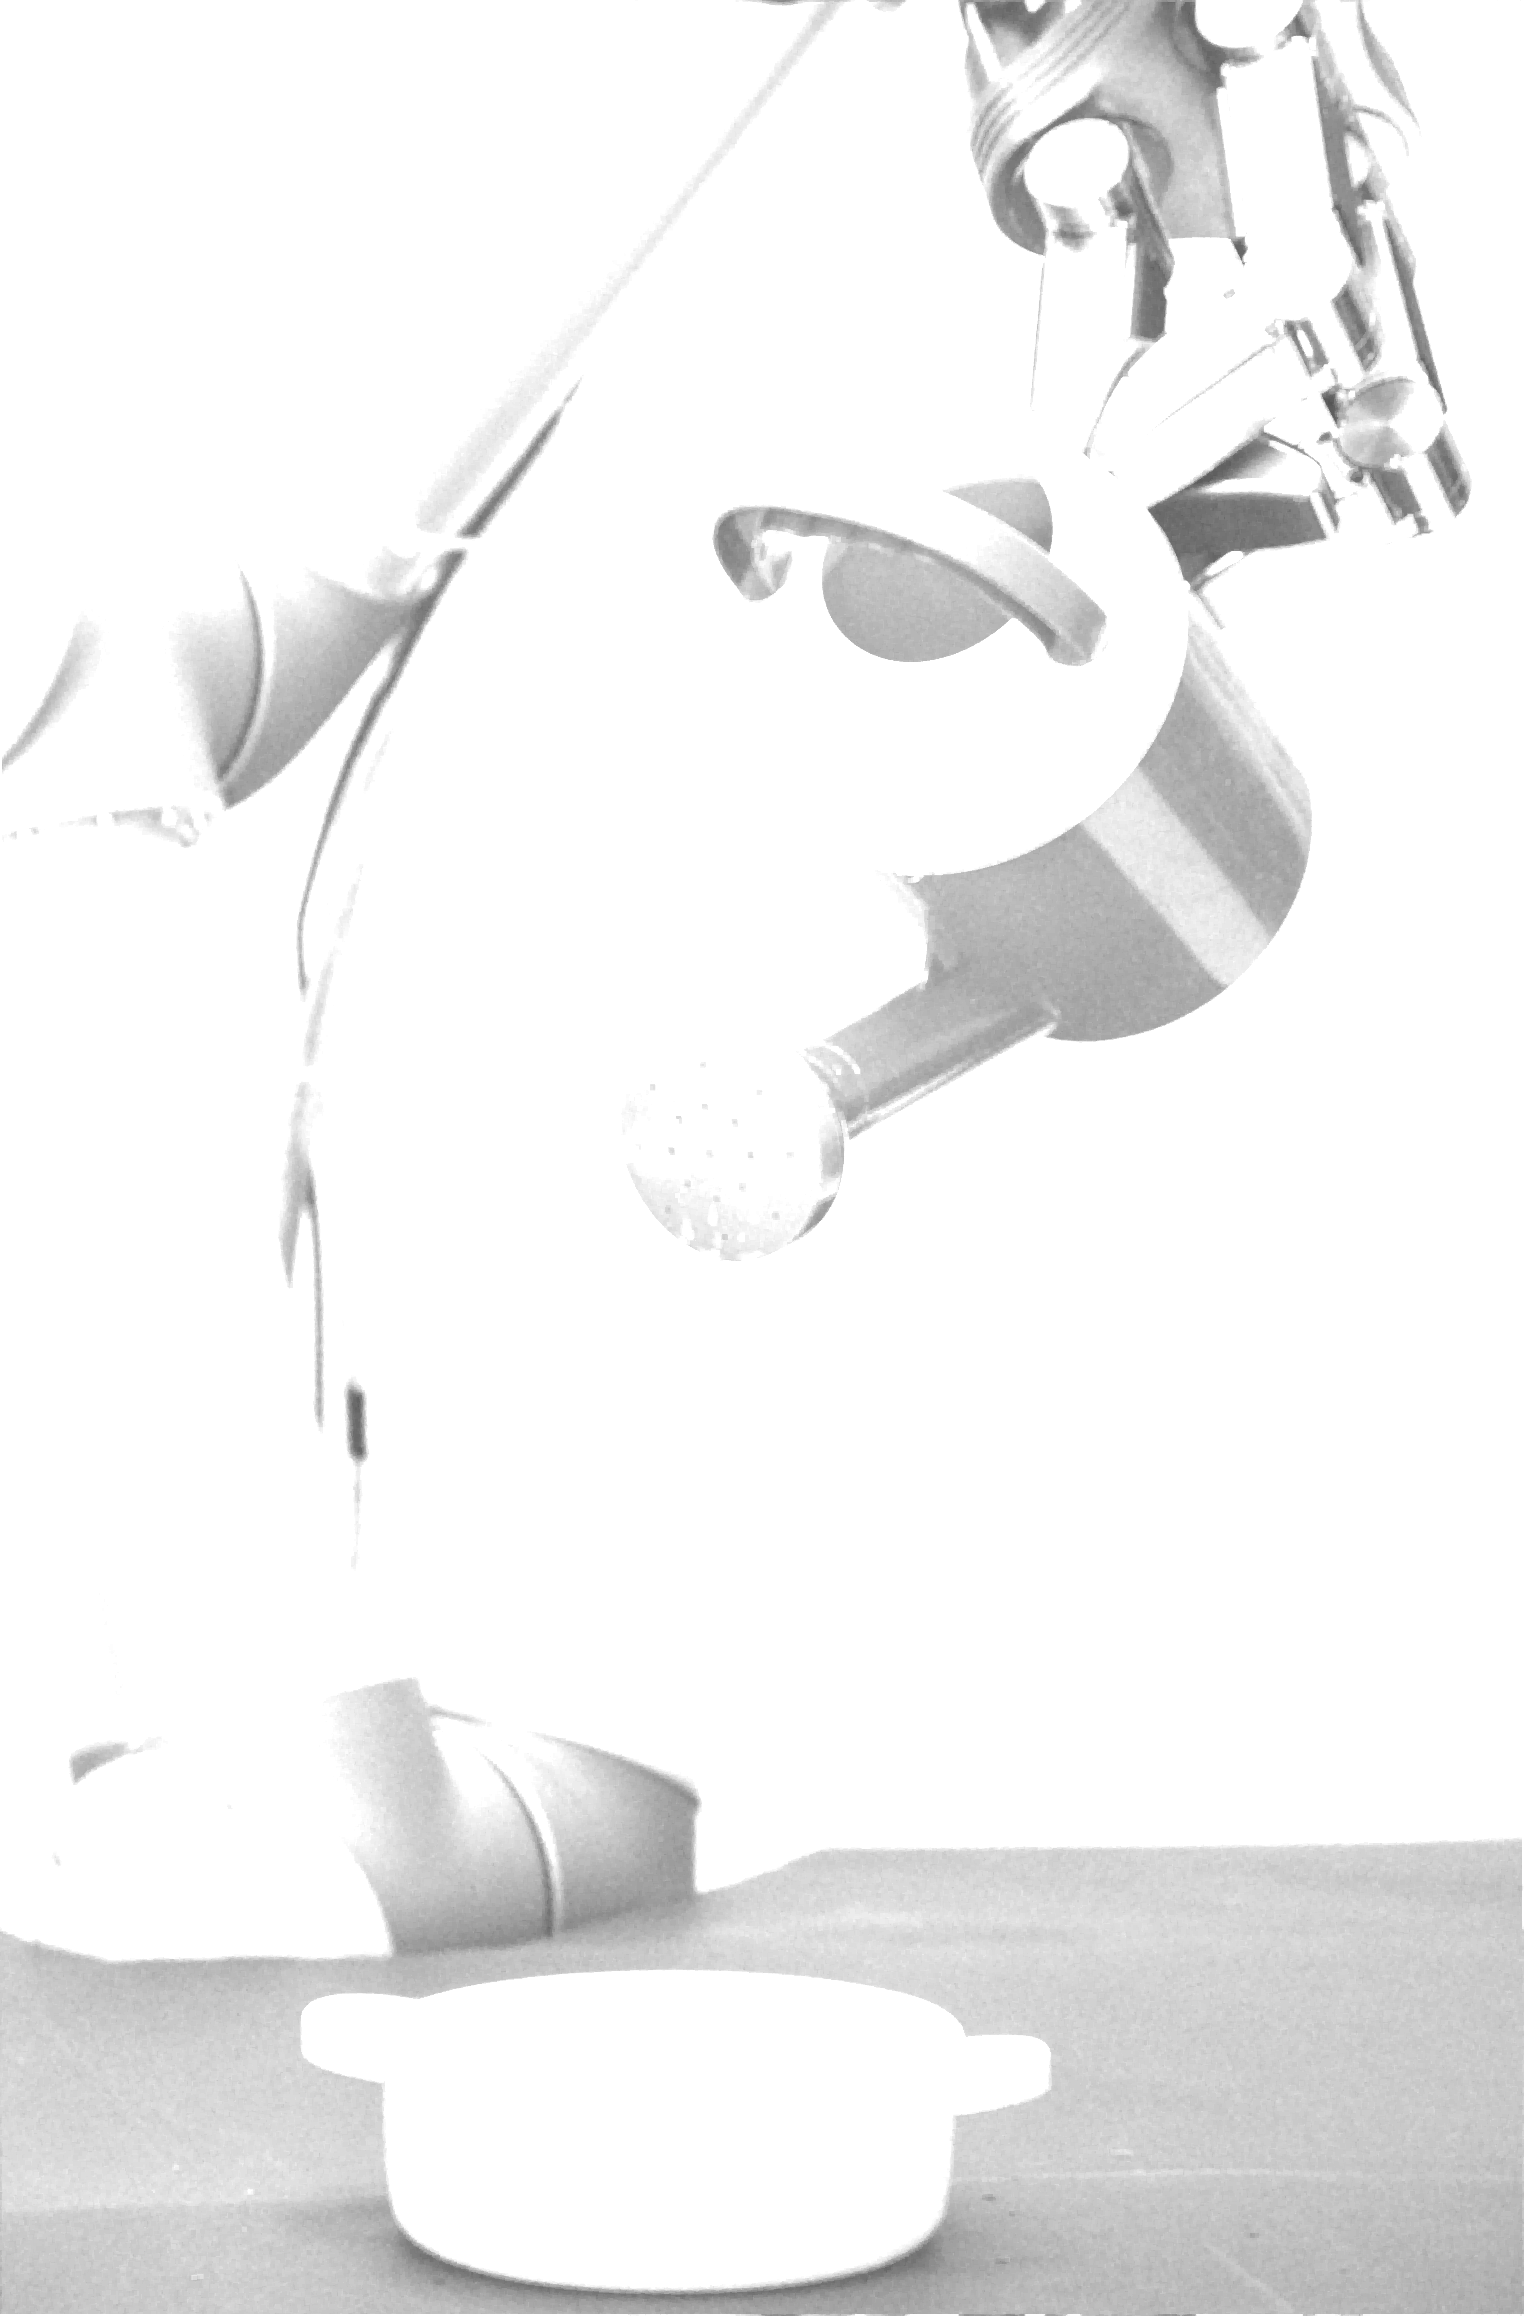
\includegraphics[width=\textwidth]{img3/test/contrast_5_1_9_final_img3.png}
    \end{subfigure}
    \caption{Testing for the right brightness}
    \label{fig:img3_test_brightness}
\end{figure} 

\begin{figure}[H]
    \centering
    \begin{subfigure}[b]{0.28\textwidth}
        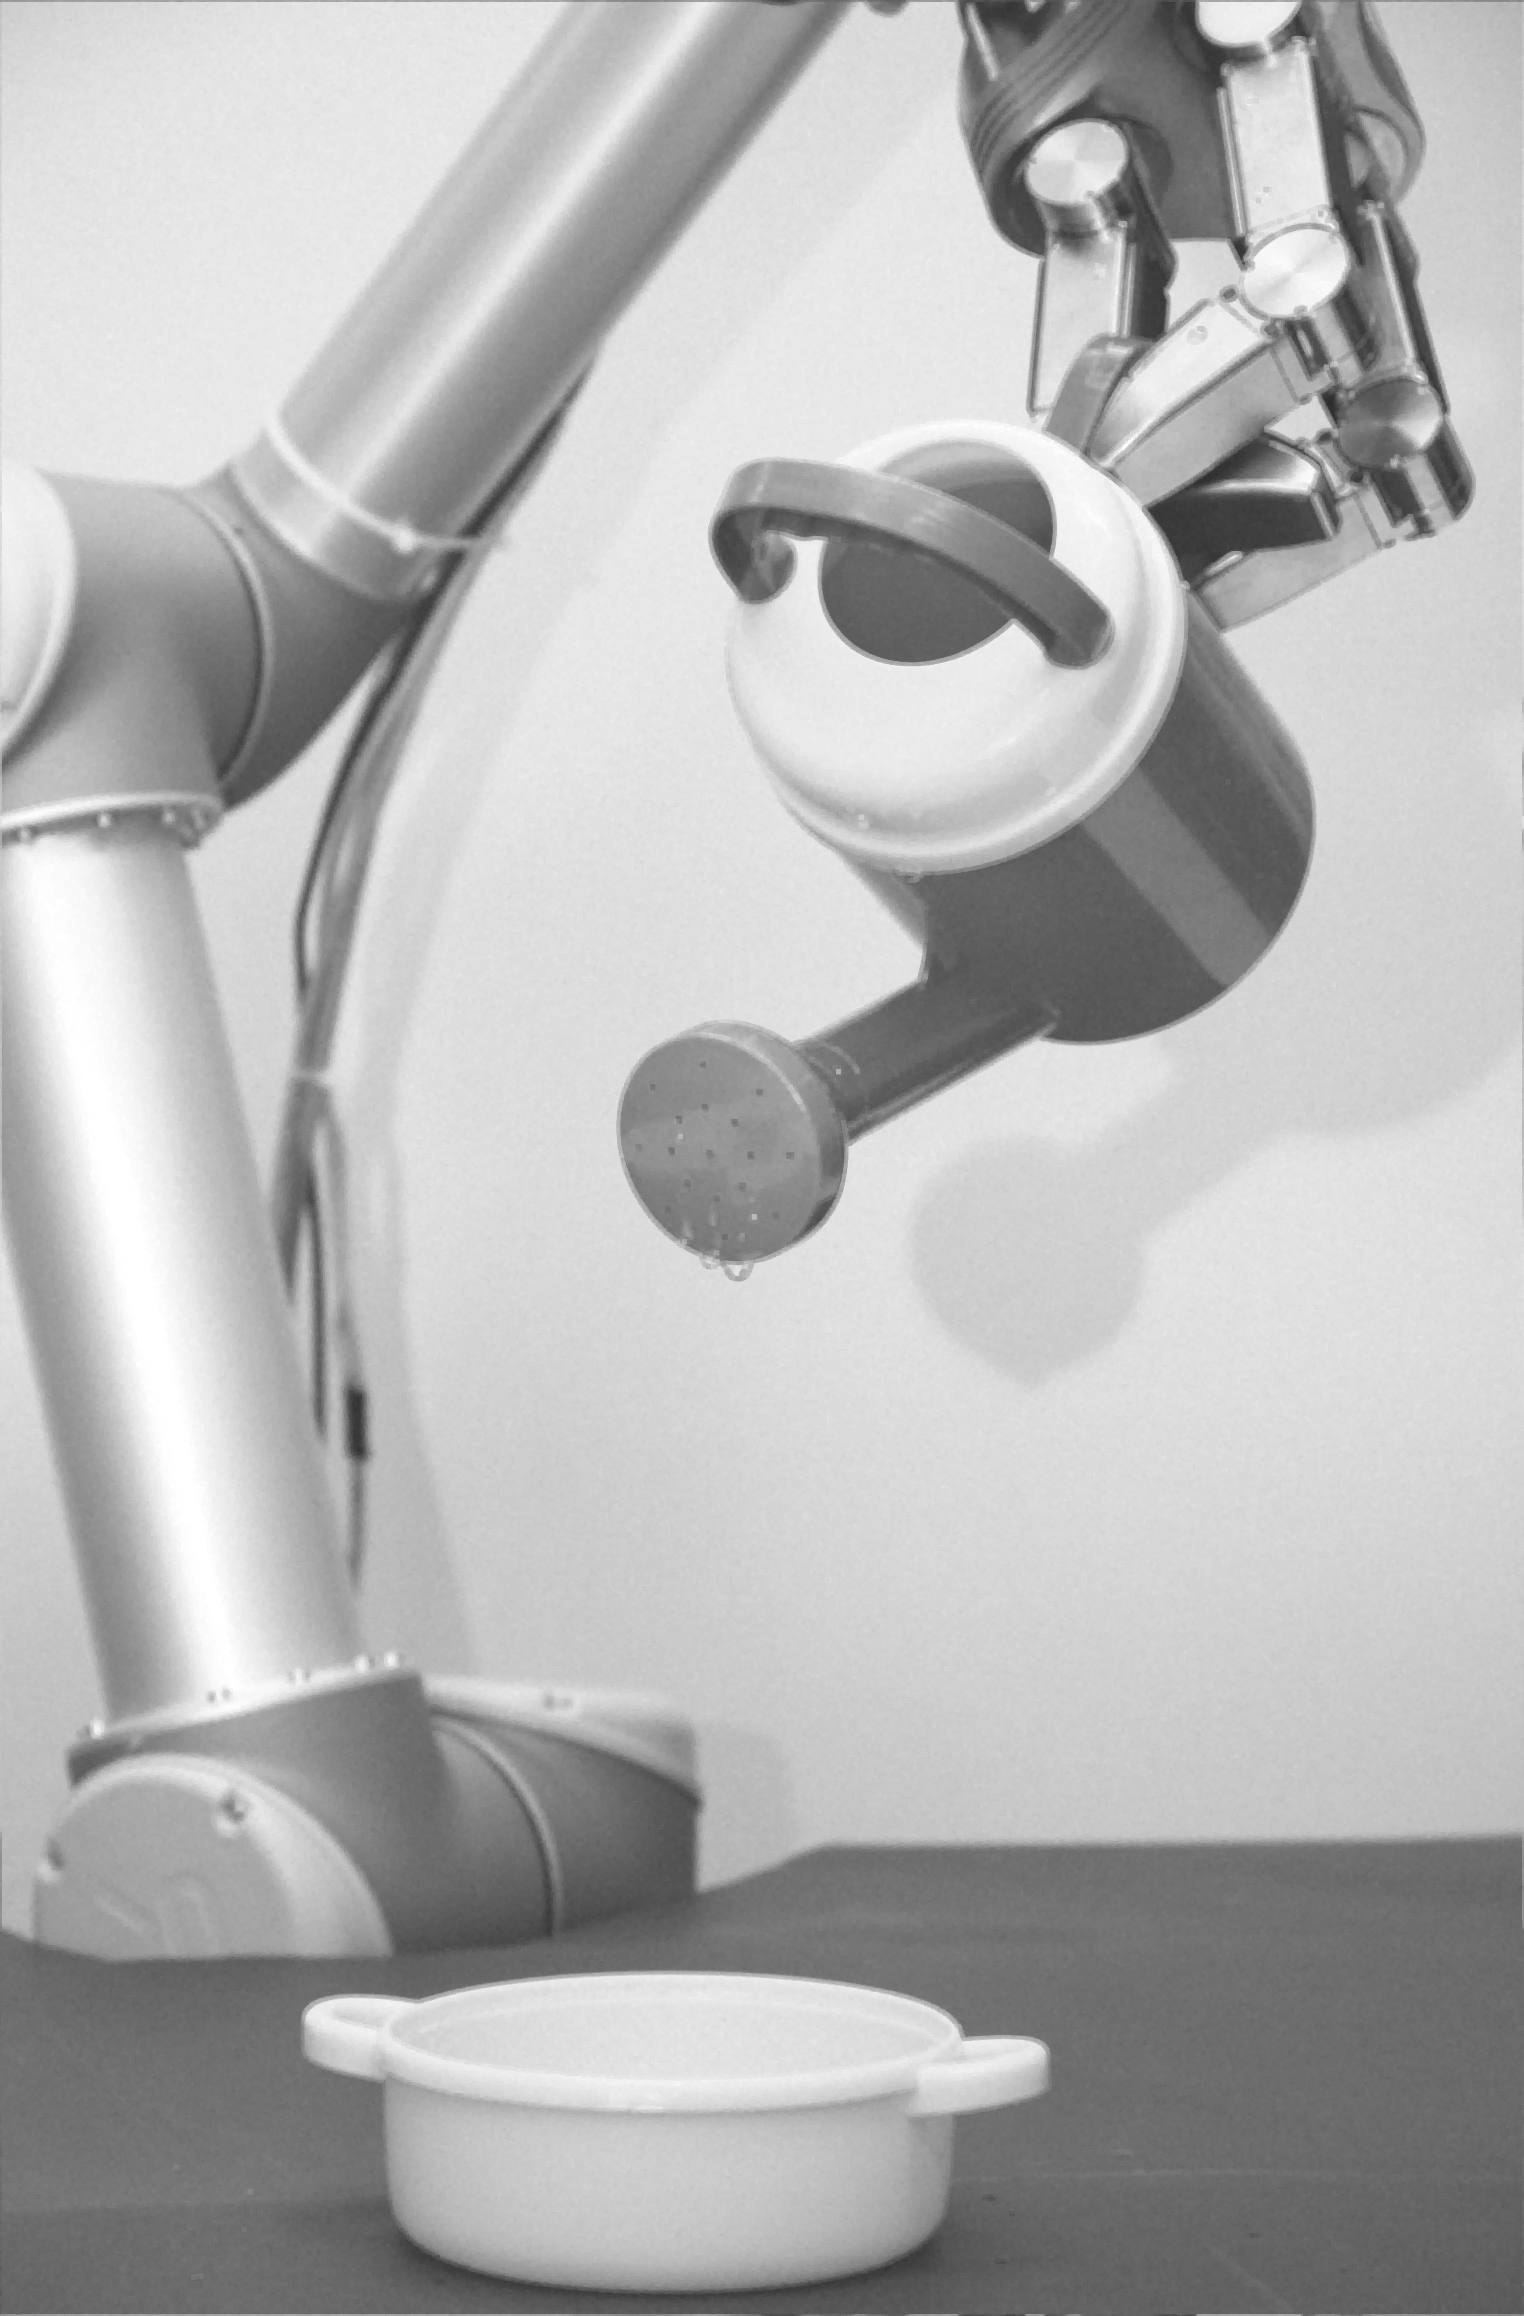
\includegraphics[width=\textwidth]{img3/midpoint_5_final_img3.png}\\[0.1cm]
        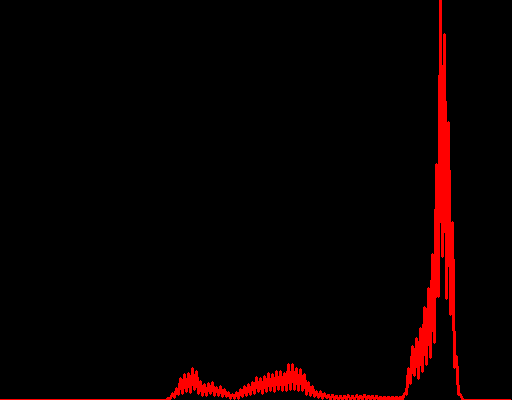
\includegraphics[width=\textwidth]{img3/hist_rect_5_midpoint_5_final_img3_org.png}
        \begin{center}
        	\textbf{Uniform surfaces}
        \end{center}
        
\includegraphics[width=\textwidth]{img3/rect_5_midpoint_5_final_img3.png}\\[0.1cm]
        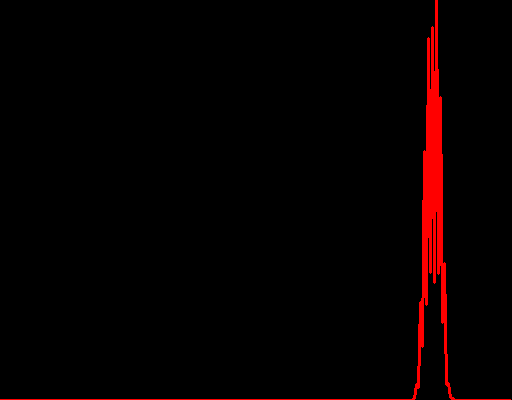
\includegraphics[width=\textwidth]{img3/hist_rect_5_midpoint_5_final_img3.png}
        \caption{Kernel 5}
        \label{fig:img3_kernel_5_final}
    \end{subfigure}
    \begin{subfigure}[b]{0.28\textwidth}
        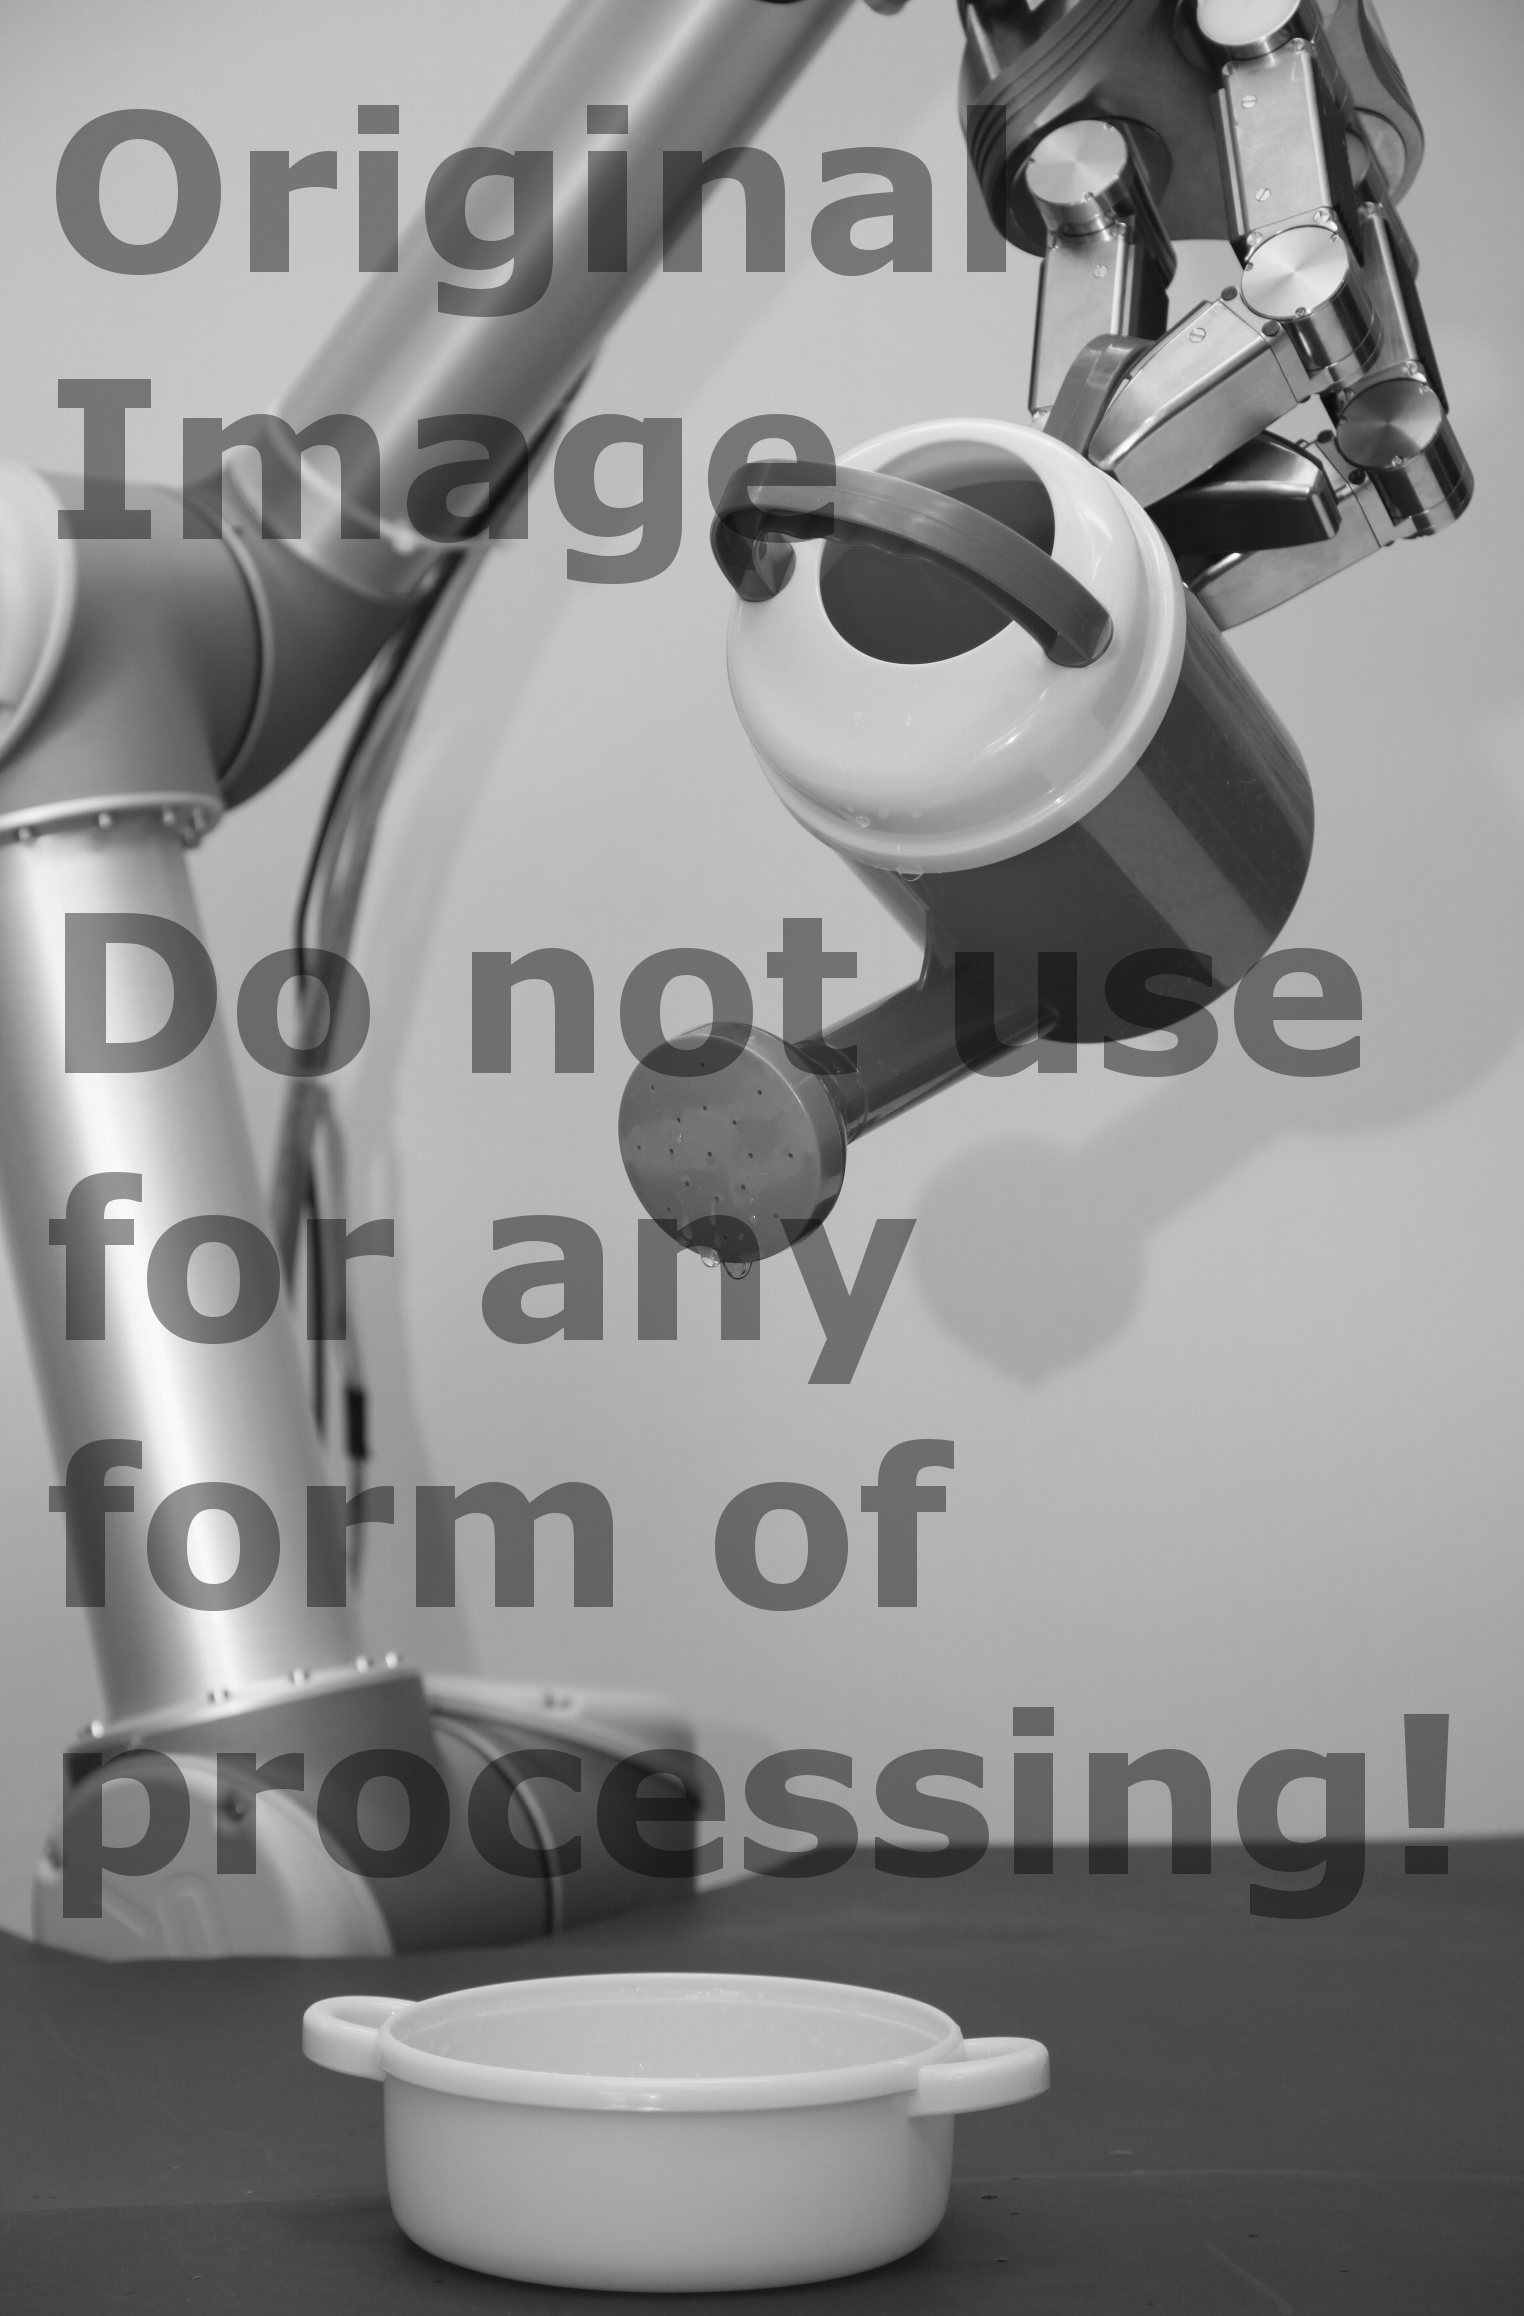
\includegraphics[width=\textwidth]{org.png}\\[0.1cm]
        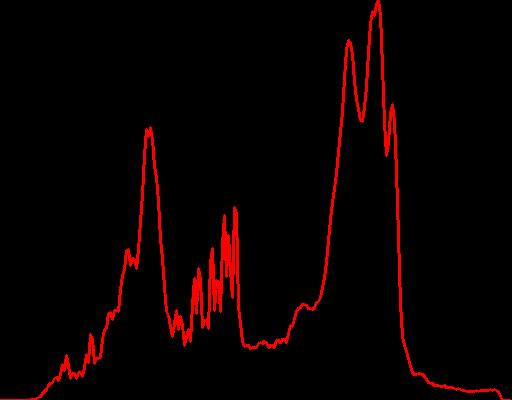
\includegraphics[width=\textwidth]{img2/hist_eee_org_res_total.png}
        \begin{center}
        	\text{ }
        \end{center}
        
\includegraphics[width=\textwidth]{img2/rect_eee_org_res_total.png}\\[0.1cm]
        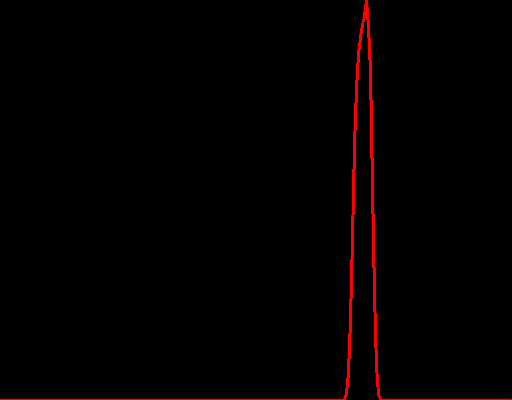
\includegraphics[width=\textwidth]{img2/hist_rect_eee_org_res_total.png}
        \caption{Original}
        \label{fig:img3_org_final}
    \end{subfigure}
    \begin{subfigure}[b]{0.28\textwidth}
        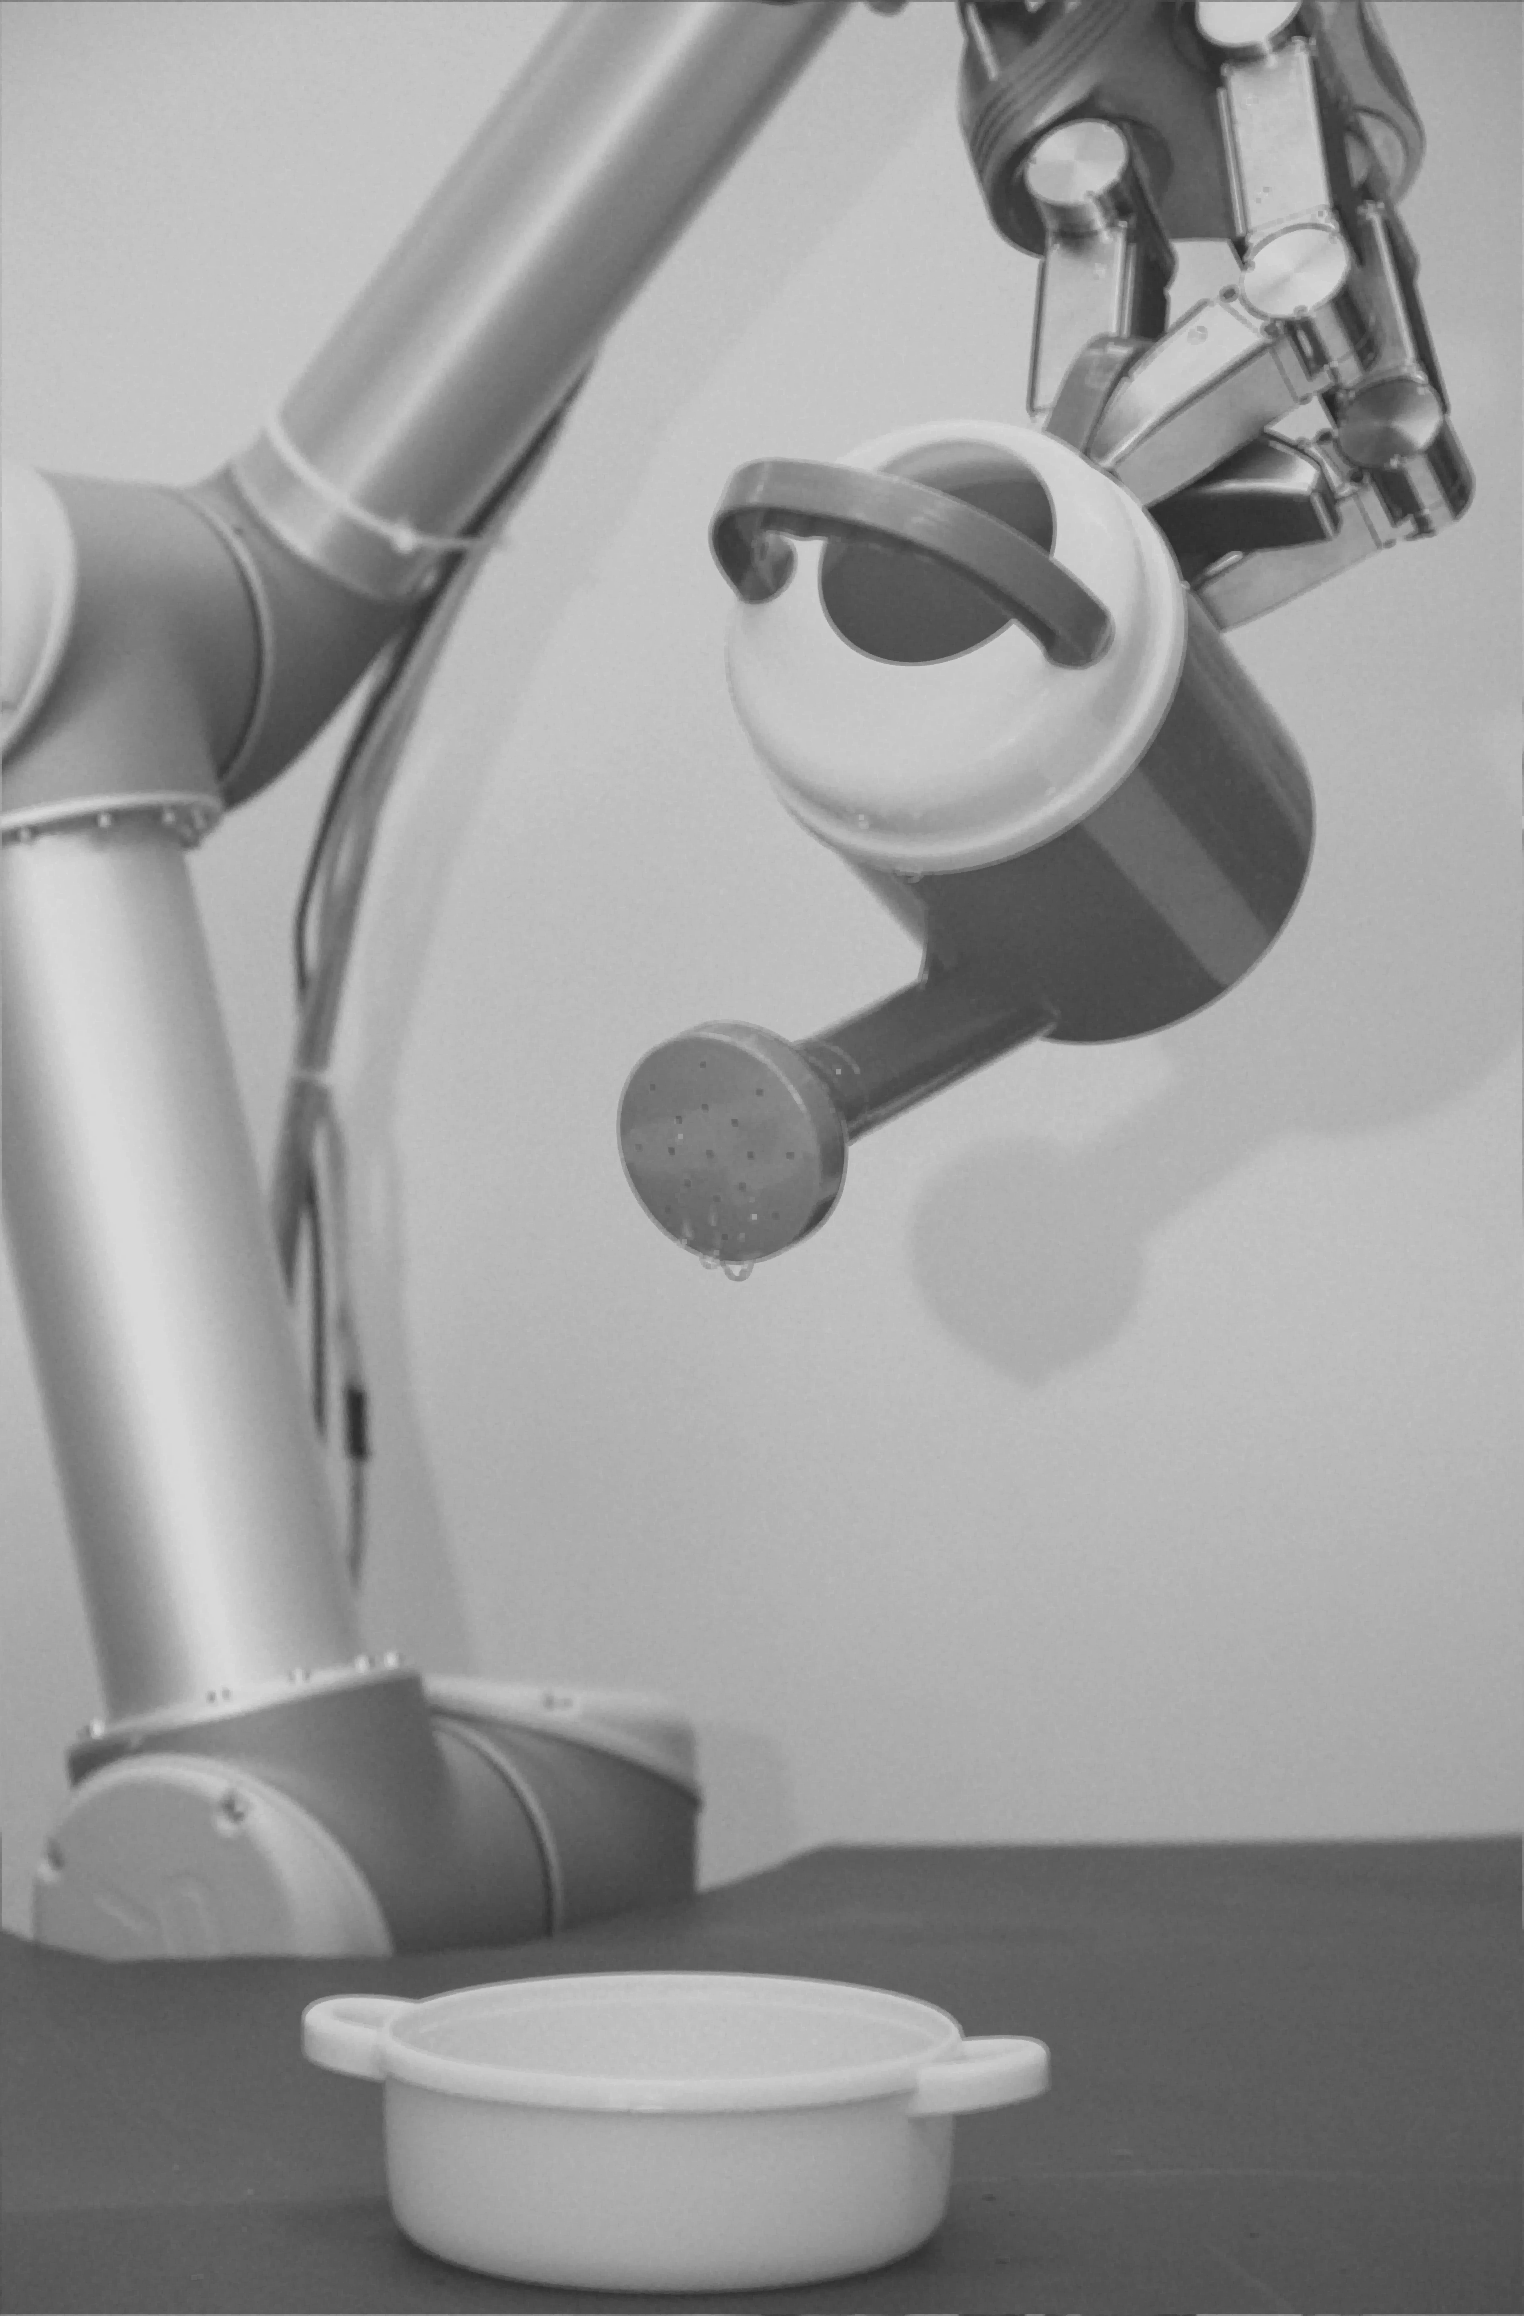
\includegraphics[width=\textwidth]{img3/contrast_5_0_85_final_img3.png}\\[0.1cm]
        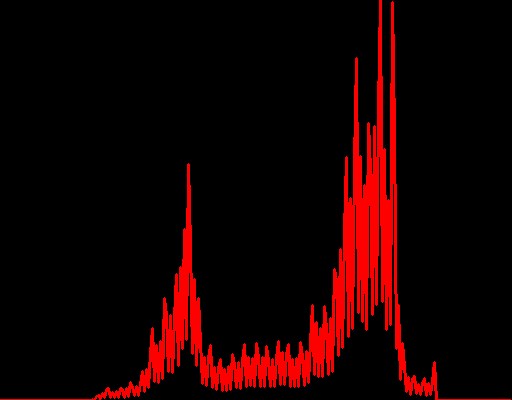
\includegraphics[width=\textwidth]{img3/hist_0_85_contrast_5_0_85_final_img3.png}
        \begin{center}
        	\text{ }
        \end{center}
        
\includegraphics[width=\textwidth]{img3/rect_0_85_contrast_5_0_85_final_img3.png}\\[0.1cm]
        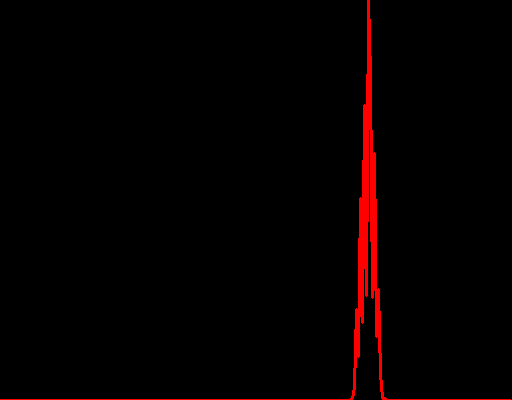
\includegraphics[width=\textwidth]{img3/hist_rect_0_85_contrast_5_0_85_final_img3.png}
        \caption{\lstinline|converTo| with 0.85}
        \label{fig:img3_contrast}
    \end{subfigure}
    \caption{Examples of different noise models}
    \label{fig:noise_examples_img3}
\end{figure} 

\todo{lidt forvirret omkring konklussionen.. hvad er dit endelig svar?}
